% !TEX encoding = IsoLatin                     
%cette premiÃère ligne permet au compilateur (souvent, dÃépend du compilateur) \LaTeX de reconnaitre l'encodage de votre fichier. 
%\documentclass[12pt,titlepage,twoside]{book}       %pour un livre
%\documentclass{report}
\documentclass[a3, 10pt,twoside]{article}          %pour un article
%\documentclass[twocolumn,amsfonts,showpacs,superscriptaddress,nofootinbib,aps,nolongbibliography]{revtex4-2}
%\documentclass[onecolumn,amsfonts,showpacs,superscriptaddress]{revtex4-1}

\usepackage{array,multirow,graphicx}
\usepackage[T1]{fontenc}  % For correct {}s in \texttt
\usepackage{accents}
\usepackage[francais]{babel}
\usepackage{amssymb, amssymb, amsthm}
\usepackage[utf8]{inputenc}             
\usepackage{amstext, amsfonts, a4}
\usepackage{pgf,pgfarrows,pgfautomata,pgfheaps,pgfnodes,pgfshade}
\usepackage[left=0.05cm,right=0.05cm,top=0.05cm,bottom=0.05cm,nohead]{geometry}
\usepackage{natbib}
%\usepackage{amsmath,amssymb}
\usepackage[pdfborder={0 0 0}]{hyperref}
\usepackage{xxcolor}
\usepackage{amscd}
\usepackage{dsfont}
\usepackage{float} 
\usepackage[Glenn]{fncychap} % Rejne Glenn\chapter
%\usetikzlibrary{circuits.ee.IEC}
\usepackage{lipsum} % pour générer du texte aléatoire

%\usepackage[tikz]{bclogo}
\usepackage{mathrsfs}%lagrangien
\usepackage{stmaryrd} %\llbracket
\usepackage{bbold}%Matrice 11
\usepackage{shapepar}
\usepackage{cancel}
\usepackage{bm}
\usepackage{pdfpages}
\usepackage[utf8]{inputenc}
\usepackage{marvosym}
\usepackage{enumitem}
\usepackage{import} % Charger le package import
\usepackage{listings} % Pour afficher du code MATLAB
\usepackage{pgfplots}
\usetikzlibrary {datavisualization}
\usetikzlibrary {arrows.meta,bending,positioning}
\usetikzlibrary {datavisualization.formats.functions}

\usepackage{tikz}
\usepackage[europeanresistor]{circuitikz}
\usepgflibrary {shadings}
%\usetikzlibrary{calc}
\usetikzlibrary{hobby, decorations.markings, arrows.meta}
\usetikzlibrary{decorations.markings} 
\usetikzlibrary{calc,intersections,through,backgrounds}
\usetikzlibrary {arrows.meta}


%%%%%%%%%%%%%%%%%%%%%%%%%%%%%%%%% Pour le tag
%\usepackage[utf8]{inputenc}
%\usepackage{fourier}
\usepackage{mathtools}
%\usepackage{cleveref}
\usepackage{xcolor}
\usepackage{graphicx}
\usepackage{enumitem} % Pour personnaliser les listes
\usepackage{caption} % Pour personnaliser les légendes des figures
\usepackage{xcolor}


%%%%%%%%%%%%%%%%%%%%%%%%%%%%%%%%%%


%%%%%%%%%%%%%%%%%%%%%%%%%%%%%%%%%%
\newcommand{\operatorvec}[1]{\hat{{\bm{#1}}}} % pour les operateur
\newcommand{\operator}[1]{\hat{\bm{#1}}} % pour les operaeur vecteur 
\newcommand{\operatortilde}[1]{\tilde{\bm{#1}}} % pour les opetateur avec un tilde
\newcommand{\operatortildevec}[1]{\tilde{\bm{#1}}}% pour les opetateur avec un tilde et vecteur 
%%%%%%%%%%%%%%%%%%%%%%%%%%%%%%%%%%

%\usepackage{tzplot}

%\usepakage{pstriks}
\usepackage[utf8]{inputenc}

%PREAMBULE pour schÃéma
\usepackage{pgfplots}
\usepackage{tikz}
%\usepackage[european resistor, european voltage, european current]{circuitikz}
%\usetikzlibrary{arrows,shapes,positioning}
%\usetikzlibrary{decorations.markings,decorations.pathmorphing,decorations.pathreplacing}
%\usetikzlibrary{calc,patterns,shapes.geometric}
\usetikzlibrary{patterns} % Pour les motifs comme les lignes diagonales
\usepackage{float} % Pour le placement 'H'
%FIN PREAMBULE

% PREAMBULE pour vercteur derivÃé
\usepackage[b]{esvect}    % For \vv

%\usepackage{caption}
%\usepackage{subcaption}

%\usepackage{graphicx}

\usepackage{fullpage}
\usepackage{eso-pic}
\usepackage{enumitem}

%\usepackage{pgfplots}
%\pgfplotsset{compat=1.17}



% --- Macro \xvec
\makeatletter
\newlength\xvec@height%
\newlength\xvec@depth%
\newlength\xvec@width%
\newcommand{\xvec}[2][]{%
  \ifmmode%
    \settoheight{\xvec@height}{$#2$}%
    \settodepth{\xvec@depth}{$#2$}%
    \settowidth{\xvec@width}{$#2$}%
  \else%
    \settoheight{\xvec@height}{#2}%
    \settodepth{\xvec@depth}{#2}%
    \settowidth{\xvec@width}{#2}%
  \fi%
  \def\xvec@arg{#1}%
  \def\xvec@dd{:}%
  \def\xvec@d{.}%
  \raisebox{.2ex}{\raisebox{\xvec@height}{\rlap{%
    \kern.05em%  (Because left edge of drawing is at .05em)
    \begin{tikzpicture}[scale=1]
    \pgfsetroundcap
    \draw (.05em,0)--(\xvec@width-.05em,0);
    \draw (\xvec@width-.05em,0)--(\xvec@width-.15em, .075em);
    \draw (\xvec@width-.05em,0)--(\xvec@width-.15em,-.075em);
    \ifx\xvec@arg\xvec@d%
      \fill(\xvec@width*.45,.5ex) circle (.5pt);%
    \else\ifx\xvec@arg\xvec@dd%
      \fill(\xvec@width*.30,.5ex) circle (.5pt);%
      \fill(\xvec@width*.65,.5ex) circle (.5pt);%
    \fi\fi%
    \end{tikzpicture}%
  }}}%
  #2%
}
\makeatother

% --- Override \vec with an invocation of \xvec.
\let\stdvec\vec
\renewcommand{\vec}[1]{\xvec[]{#1}}
% --- Define \dvec and \ddvec for dotted and double-dotted vectors.
\newcommand{\dvec}[1]{\xvec[.]{#1}}
\newcommand{\ddvec}[1]{\xvec[:]{#1}}
% FIN PREAMBULE


\def\pgf{\textsc{pgf}}
\def\pstricks{\textsc{pstricks}}
\def\Class#1{\hbox{\small#1}}
\def\bs{$\backslash$}

\def\Environment#1{\par\bigskip\noindent\textbf{Environment \texttt{#1}}\par}
\def\Command#1{\par\bigskip\noindent\textbf{Command \texttt{#1}}\par}
\long\def\Parameters#1{\medskip\noindent Parameters:
  \begin{enumerate}\itemsep=0pt\parskip=0pt
    #1
  \end{enumerate}}
\long\def\Description#1{\unskip\medskip\noindent Description: #1}
\def\Example{\par\medskip\noindent Example: }


\renewcommand*\descriptionlabel[1]{\hspace\labelsep\normalfont #1}


\def\declare#1{{\color{red!75!black}#1}}

\def\command#1{\list{}{\leftmargin=2em\itemindent-\leftmargin\def\makelabel##1{\hss##1}}%
\item\extractcommand#1@\par\topsep=0pt}
\def\endcommand{\endlist}
\def\extractcommand#1#2@{\strut\declare{\texttt{\string#1}}#2}


\def\environment#1{\list{}{\leftmargin=2em\itemindent-\leftmargin\def\makelabel##1{\hss##1}}%
\extractenvironement#1@\par\topsep=0pt}
\def\endenvironment{\endlist}
\def\extractenvironement#1#2@{%
\item{{\ttfamily\char`\\begin\char`\{\declare{#1}\char`\}}#2}%
  {\itemsep=0pt\parskip=0pt\item{\meta{environment contents}}%
  \item{\ttfamily\char`\\end\char`\{\declare{#1}\char`\}}}}


\def\smallpackage{\vbox\bgroup\package}
\def\endsmallpackage{\egroup\endpackage}
\def\package#1{\list{}{\leftmargin=2em\itemindent-\leftmargin\def\makelabel##1{\hss##1}}%
\extracttheme#1@\par\topsep=0pt}
\def\endpackage{\endlist}
\def\extracttheme#1#2@{%
\item{{{\ttfamily\char`\\usepackage}#2{\ttfamily\char`\{\declare{#1}\char`\}}}}}



\def\Environment#1{\par\bigskip\noindent\textbf{Environment \texttt{#1}}\par}
\def\Command#1{\par\bigskip\noindent\textbf{Command \texttt{#1}}\par}
\long\def\Parameters#1{\medskip\noindent Parameters:
  \begin{enumerate}\itemsep=0pt\parskip=0pt
    #1
  \end{enumerate}}
\long\def\Description#1{\unskip\medskip\noindent Description: #1}
\def\Example{\par\medskip\noindent Example: }

\newcommand{\w}[1]{\bf{#1}}\newcommand{\ww}[1]{\bf{#1}}
%\newcommand{\w}[1]{\vec{#1}}\newcommand{\ww}[1]{\overrightarrow{#1}}



\newcommand{\vertiii}[1]{{\left\vert\kern-0.25ex\left\vert\kern-0.25ex\left\vert#1\right\vert\kern-0.25ex\right\vert\kern-0.25ex\right\vert}}

%%%%%%%%%%%%%%%%%%%%%%%%%%%%%%%%%%%%%%%%%%%%%%%%%%%%%%%%%%%
    %%%%%%%% Accent Math
%%%%%%%%%%%%%%%%%%%%%%%%%%%%%%%%%%%%%%%%%%%%%%%%%%%%%%%%%%%
\makeatletter
\newcommand*{\math@auxii}[2][3]{{}\mkern#1mu\overline{\mkern-#1mu#2}}
\newcommand*{\math@auxi}[3][3]{\overset{\mkern#1mu\text{\scalebox{0.7}{#3}}\mkern-#1mu}{\smash{\math@auxii[#1]{#2}}\vphantom{#2}}}
\newcommand*{\mathco}[2][3]{\math@auxi[#1]{#2}{$\circ$}}
\newcommand*{\mathabc}[2][3]{\math@auxi[#1]{#2}{abc}}
\makeatother

%%%%%%%%%%%%%%%%%%%%%%%%%%%%%%%%%%%%%%%%%%%%%%%%%%%%%%%%%
%%%%algorithmes / pseudo code%%%
%%%%%%%%%%%%%%%%%%%%%%%%%%%%%%%%%%%%%%%%%%%%%%%%%%%%%%%%%%
\usepackage[french,ruled]{algorithm2e}

%%%%%
\usepackage{color,transparent}
%%%%%
%\usepackage{graphics,graphicx,subfigure,caption}
%\usepackage{graphics,graphicx,caption}
\usepackage{caption}
\usepackage{subcaption}
\usepackage{comment}
\usepackage{float} 
\setcounter{MaxMatrixCols}{30}%

%%%%%%%%%%%%%%%%%%%%%%%%%%%%%%%%%%%%%%%%
%%%%        Dimensions du texte (à adapter selon votre goût/le goût de l'Ãéditeur)
%%%%%%%%%%%%%%%%%%%%%%%%%%%%%%%%%%%%%%%%

\setlength\textwidth{19cm}          % largeur du texte
\setlength\topmargin{-2cm}          % marge en haut
\setlength\evensidemargin{-1cm}     % marge de gauche
\setlength\textheight{24cm}         % hauteur du texte
\setlength\oddsidemargin{\evensidemargin}

%%%%%%%%%%%%%%%%%%%%%%%%%%%%%%%%%%%%%%%%
%         D\'ecoupage des mots           %
%%%%%%%%%%%%%%%%%%%%%%%%%%%%%%%%%%%%%%%%
\hyphenation{}

%%%%%%%%%%%%%%%%%%%%%%%%%%%%%%%%%%%%%%%%
%%%%  Th\'eor\`emes, d\'efinitions, etc.
%%%%%%%%%%%%%%%%%%%%%%%%%%%%%%%%%%%%%%%%


% Il y a diffÃérents types d'ÃénoncÃés qui mÃéritent un environnement spÃécifique, voici une liste assez exhaustive. 
\theoremstyle{plain}
	\newtheorem{Theo}{Th\'eor\`eme}[section] %compteur commençant par le numÃéro de la section (on pourrait aussi faire commencer par le numÃéro de la sous-section - remplacer "section" par "subsection")
	\newtheorem{Prop}[Theo]{Proposition}        %mÃême compteur que pour les thÃéorÃèmes      
	\newtheorem{Prob}[Theo]{Probl\`eme}	    %idem
	\newtheorem{Lemm}[Theo]{Lemme}            %etc...
	\newtheorem{Coro}[Theo]{Corollaire}
	\newtheorem{Propr}[Theo]{Propri\'et\'e}
	\newtheorem{Conj}[Theo]{ Conjecture}
	\newtheorem{Aff}[Theo]{Affirmation}

    \newtheorem{TheoPrinc}{Th\'eor\`eme}     %compteur spÃécifique pour les thÃéorÃèmes les plus importants du papier
        
\theoremstyle{definition}
	\newtheorem{Defi}[Theo]{D\'efinition}
    \newtheorem{Exem}[Theo]{Exemple}
	\newtheorem{Nota}[Theo]{\Large Notation}

\theoremstyle{remark}
	\newtheorem{Rema}[Theo]{Remarque}
	\newtheorem{NB}[Theo]{N.B.}
	\newtheorem{Comm}[Theo]{Commentaire}
	\newtheorem{question}[Theo]{$\ast$ Question}
	\newtheorem{exer}[Theo]{Exercice}
	\newtheorem{Consequence}[Theo]{Conséquence}
	\newtheorem{Rap}[Theo]{Rappel}
	\newtheorem*{Merci}{Remerciements}
	
\usepackage{mdframed}

\mdfdefinestyle{propstyle}{%
linecolor=black,linewidth=2pt,%
hidealllines=true,
frametitlerule=true,%
frametitlebackgroundcolor=gray!20,
backgroundcolor=gray!10!white,
roundcorner=5pt,
innertopmargin=\topskip,
}

%\mdtheorem[style=propstyle]{prop}{Property}[chapter]
\mdtheorem[style=propstyle]{lemma}[prop]{Lemma}
\mdtheorem[style=propstyle]{TheoPrinc}{Th\'eor\`eme}[chapter]

% Définition d'un style personnalisé pour les Affirmations
\mdfdefinestyle{affirmestyle}{%
    linecolor=gray, % Couleur de la bordure
    linewidth=1pt, % Épaisseur de la bordure
    backgroundcolor=gray!10, % Couleur de fond (gris clair)
    roundcorner=5pt, % Coins arrondis
    innertopmargin=\topskip, % Marge intérieure
    skipabove=10pt, % Espace au-dessus du cadre
    skipbelow=10pt % Espace en-dessous du cadre
}

% Définition de l'environnement Affirmation
\theoremstyle{definition} % Style de théorème pour les affirmations
\newmdtheoremenv[style=affirmestyle]{aff}{Affirmation} % Environnement Affirmation avec le style personnalisé


	

%%%%%%%%%%%%%%%%%%%%%%%%%%%%%%%%%%%%%%%%
%%%%  Accolades, guillemets, etc.
%%%%%%%%%%%%%%%%%%%%%%%%%%%%%%%%%%%%%%%%

\def\ogg~{{\rm \og}}   % guillemets ouvrants
\def\fgg{{\rm \fg}}  % guillemets fermants



\def\nl{\newline}
\def\nn{\noindent}

\def\q{\nn}
\def\qq{\nn\quad}
\def\qqq{\nn\quad\quad}
\def\qqqq{\nn\quad\quad\quad}
\def\ce{\centerline}

%%%%%%%%%%%%%%%%%%%%%%%%%%%%%%%%%%%%%%%%
%%%%  Lettres et symboles math\'ematiques
%%%%%%%%%%%%%%%%%%%%%%%%%%%%%%%%%%%%%%%%

\def\emptyset{\varnothing}

%%%% Raccourcis pour les caractÃères gras mathÃématiques (ensembles R, N, Z, C etc)

\def\NN{{\mathbb N}}    %naturels
\def\ZZ{{\mathbb Z}}     %entiers relatifs
\def\RR{{\mathbb R}}    %rÃéels
\def\QQ{{\mathbb Q}}    %rÃéels
\def\CC{{\mathbb C}}    %complexes
\def\HH{{\mathbb H}}    %quaternions / espace hyperbolique
\def\AA{{\mathbb P}}     %espace projectif
\def\KK{{\mathbb K}}     %corps quelconques

\def\EE{{\mathbb E}}     %Experance
\def\VV{{\mathbb V}}     %Variance

%%%%%%raccourcis lettres calligraphiÃées
\def\cA{{\mathcal A}}  \def\cG{{\mathcal G}} \def\cM{{\mathcal M}} \def\cS{{\mathcal S}} \def\cB{{\mathcal B}}  \def\cH{{\mathcal H}} \def\cN{{\mathcal N}} \def\cT{{\mathcal T}} \def\cC{{\mathcal C}}  \def\cI{{\mathcal I}} \def\cO{{\mathcal O}} \def\cU{{\mathcal U}} \def\cD{{\mathcal D}}  \def\cJ{{\mathcal J}} \def\cP{{\mathcal P}} \def\cV{{\mathcal V}} \def\cE{{\mathcal E}}  \def\cK{{\mathcal K}} \def\cQ{{\mathcal Q}} \def\cW{{\mathcal W}} \def\cF{{\mathcal F}}  \def\cL{{\mathcal L}} \def\cR{{\mathcal R}} \def\cX{{\mathcal X}} \def\cY{{\mathcal Y}}  \def\cZ{{\mathcal Z}}

%%%%%%raccourcis lettres gothiques

\def\mfA{{\mathfrak A}} \def\mfA{{\mathfrak P}} \def\mfS{{\mathfrak S}}\def\mfZ{{\mathfrak Z}} \def\mfM{{\mathfrak M}} \def\mfQ{{\mathfrak Q}} \def\mfE{{\mathfrak E}} \def\mfL{{\mathfrak L}} \def\mfW{{\mathfrak W}} \def\mfR{{\mathfrak R}} \def\mfK{{\mathfrak K}} \def\mfX{{\mathfrak X}} \def\mfT{{\mathfrak T}} \def\mfJ{{\mathfrak J}} \def\mfC{{\mathfrak C}} \def\mfY{{\mathfrak Y}} \def\mfH{{\mathfrak H}} \def\mfV{{\mathfrak V}}\def\mfU{{\mathfrak U}}\def\mfG{{\mathfrak G}} \def\mfB{{\mathfrak B}} \def\mfI{{\mathfrak I}} \def\mfF{{\mathfrak F}} \def\mfN{{\mathfrak N}} \def\mfO{{\mathfrak O}} \def\mfD{{\mathfrak D}} 

\def\mfa{{\mathfrak a}} \def\mfp{{\mathfrak p}} \def\mfs{{\mathfrak s}}  \def\mfz{{\mathfrak z}} \def\mfm{{\mathfrak m}} \def\mfq{{\mathfrak q}}  \def\mfe{{\mathfrak e}} \def\mfl{{\mathfrak l}} \def\mfw{{\mathfrak w}} \def\mfr{{\mathfrak r}} \def\mfk{{\mathfrak k}} \def\mfx{{\mathfrak x}} \def\mft{{\mathfrak t}} \def\mfj{{\mathfrak j}} \def\mfc{{\mathfrak c}} \def\mfy{{\mathfrak y}} \def\mfh{{\mathfrak h}} \def\mfv{{\mathfrak v}} \def\mfu{{\mathfrak u}} \def\mfg{{\mathfrak g}} \def\mfb{{\mathfrak b}} \def\mfi{{\mathfrak i}} \def\mff{{\mathfrak f}} \def\mfn{{\mathfrak n}} \def\mfo{{\mathfrak o}} \def\mfd{{\mathfrak d}} 



%%raccourcis texte
\newcommand{\nbh}{\nobreakdash-\hspace*{0pt}}	% trait d'union insÃécable
\newcommand{\cad}{c'est\nbh \`a\nbh dire}		% c.-??-d.
\newcommand{\Cad}{C'est\nbh \`a\nbh dire}		% C.-??-d.

%%opÃérateurs   (ajoutez les raccourcis que vous voulez pour les opÃérateurs dont avez besoin)
\newcommand{\pgcd}{\operatorname{pgcd}}
\newcommand{\ppcm}{\operatorname{ppcm}}
\newcommand{\GL}{\operatorname{GL}}             %groupe linÃéaire
\newcommand{\Sp}{\mathsf{Sp}}			    %spectre
\newcommand{\End}{\operatorname{End}}         %Endomorphismes
\newcommand\Aut{\operatorname{Aut}}		  %etc...
\newcommand\ct{\operatorname{cotan}}         %cotangente
\newcommand{\dx}{\partial_x}                    
\newcommand{\dy}{\partial_y}
\newcommand{\Ker}{\operatorname{Ker}}
\newcommand{\Id}{\operatorname{Id}}
%\def\Im{\operatorname{Im}}                            %dans ce cas, \newcommand ne va pas marcher car la commande \Im existe dÃéjà. On utilise alors  \def de tex.

%%%%% a ajouter 

\usepackage{xcolor}
\newcommand{\varitem}[3][black]{%
  \item[%
   \colorbox{#2}{\textcolor{#1}{\makebox(5.5,7){#3}}}%
  ]
}


%%%%

\usepackage{scalerel}
\usepackage{xcolor}
\usepackage{stackengine}
\usepgflibrary {shadings}


\usetikzlibrary {decorations.pathmorphing}

\newcommand\dangersign[1]{%
    \renewcommand\stacktype{L}%
    \scaleto{\stackon[1.3pt]{\color{red}$\triangle$}{\tiny !}}{#1}%
}

\usepackage{tikz}
\tikzset{every picture/.style={execute at begin picture={\shorthandoff{:;!?};}}}
\tikzstyle{every picture}+=[remember picture]
\tikzstyle{na} = [shape=rectangle,inner sep=0pt]

% Commandes pour les flèches textuelles
\newcommand{\ptFleche}[2]{		% Déclaration d'une extrémité de flèche
    \tikz[baseline=(#1.base)]\node[na](#1){#2};
  }
%\newcommand{\Fleche}[5][thick]{	% Dessin de la flèche
%    \begin{tikzpicture}[overlay]
%        \path[->,#1](#2) edge [out=#4, in=#5] (#3);
%    \end{tikzpicture}
%  }
  
% \newcommand{\Flecheprim}[5][thick]{	% Dessin de la flèche
%    \begin{tikzpicture}[overlay]
%        \path[->,#1](#2) edge [out=#4, in=#5] (#3);
%    \end{tikzpicture}
%  }
%
\usepackage{marvosym}
\usepackage{changepage}
 
\definecolor{OliveGreen}{HTML}{808000}
\def\OliveGreen{OliveGreen}

\begin{document}

	%\includegraphics[width=\textwidth]{Figures/Shema}
	
	\section{Essancielle}
		\begin{figure}[H]
			\centering
			\begin{subfigure}[b]{1\textwidth}
				\centering
				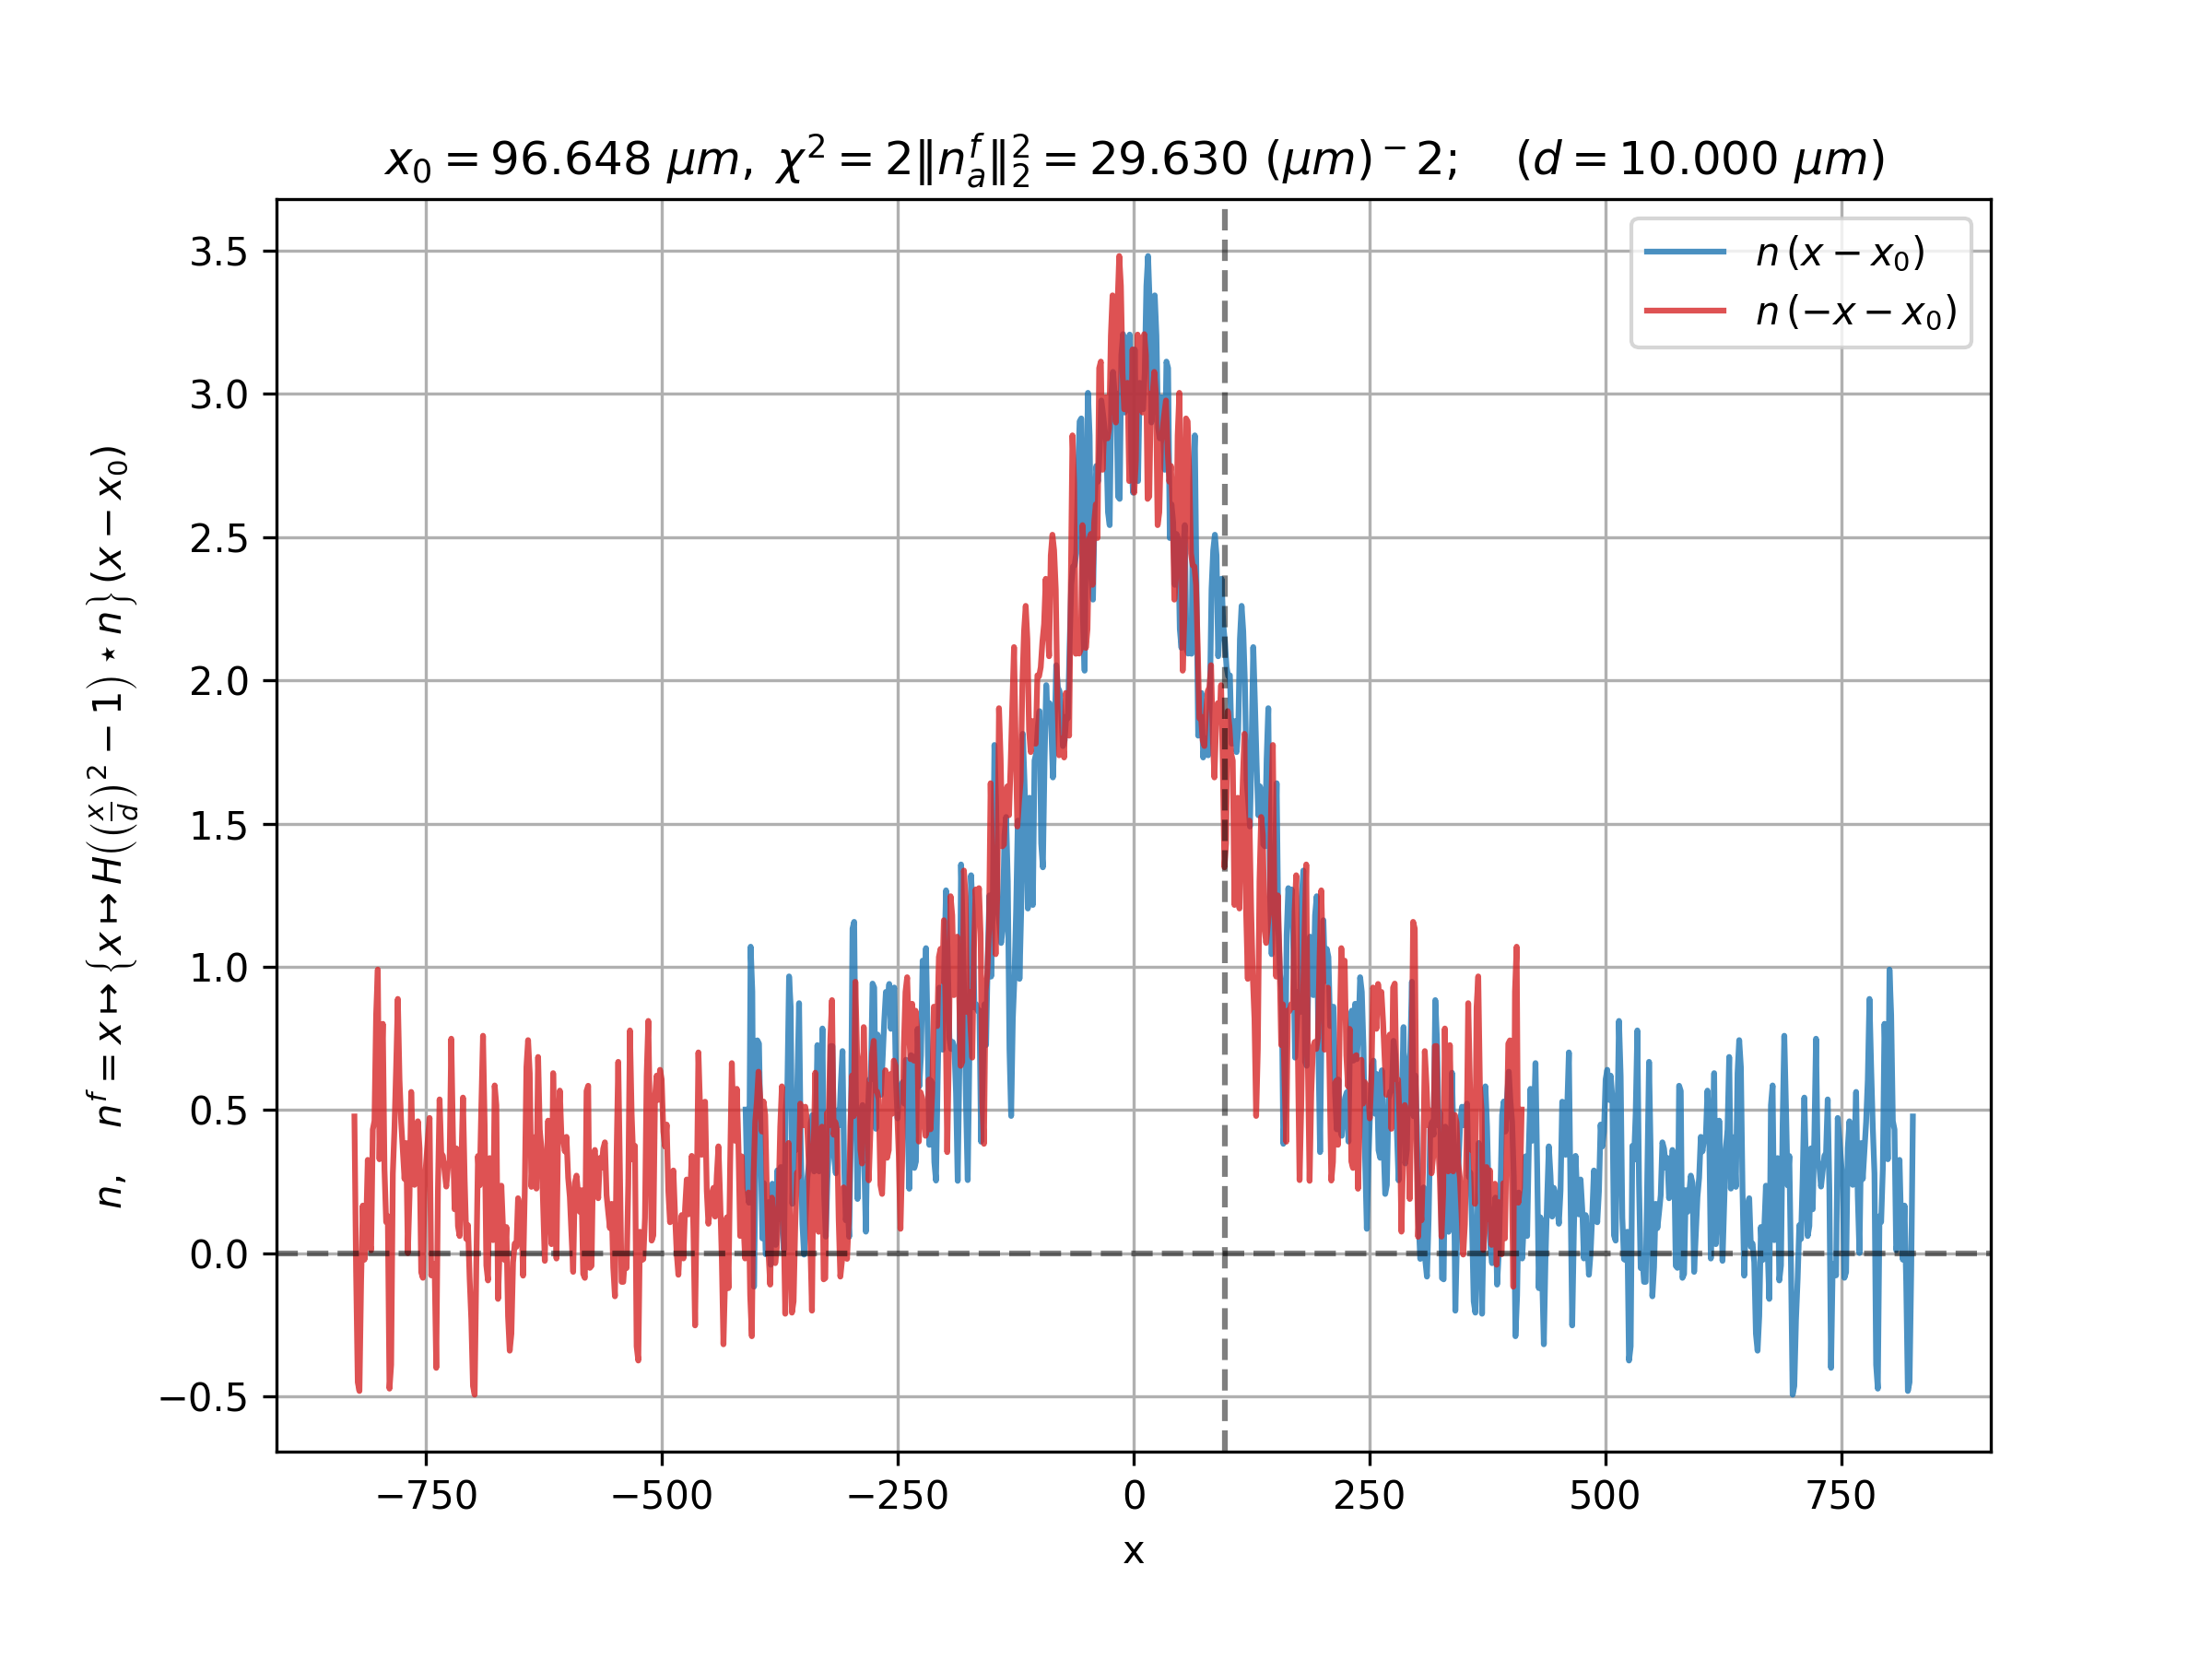
\includegraphics[width=0.48\textwidth]{Figures/article_asymetrie_09-02-2024}
				\caption{}
        		\label{}
			\end{subfigure}
			\vspace{1em}
			\begin{subfigure}[b]{0.48\textwidth}
   				 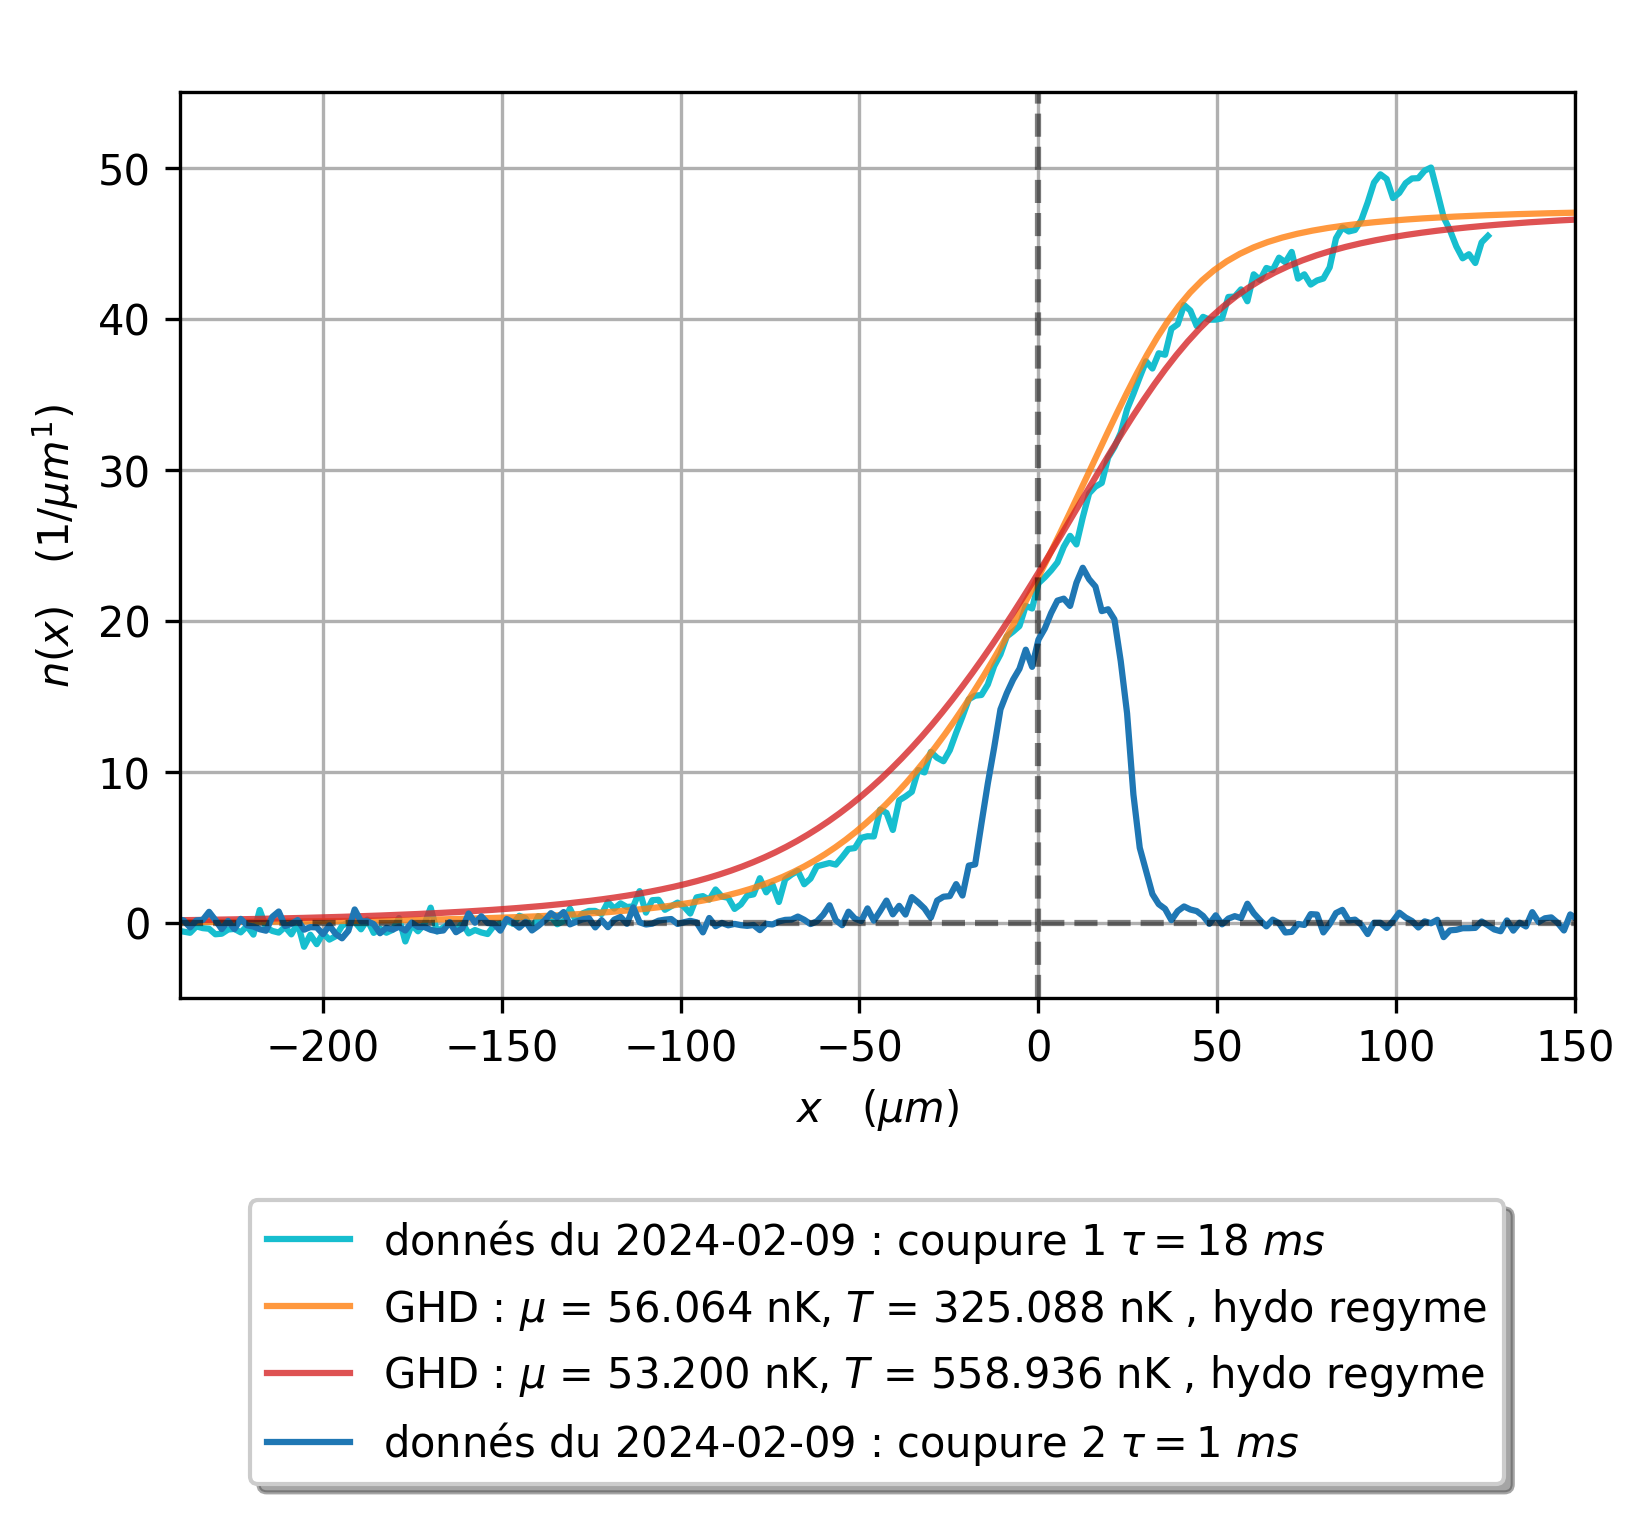
\includegraphics[width=\textwidth]{Figures/article_simul_deformation_1_09-02-2024}
        			\caption{}
        		\label{}
   			\end{subfigure}
    		\hfill
    		\begin{subfigure}[b]{0.48\textwidth}
        		\centering
        		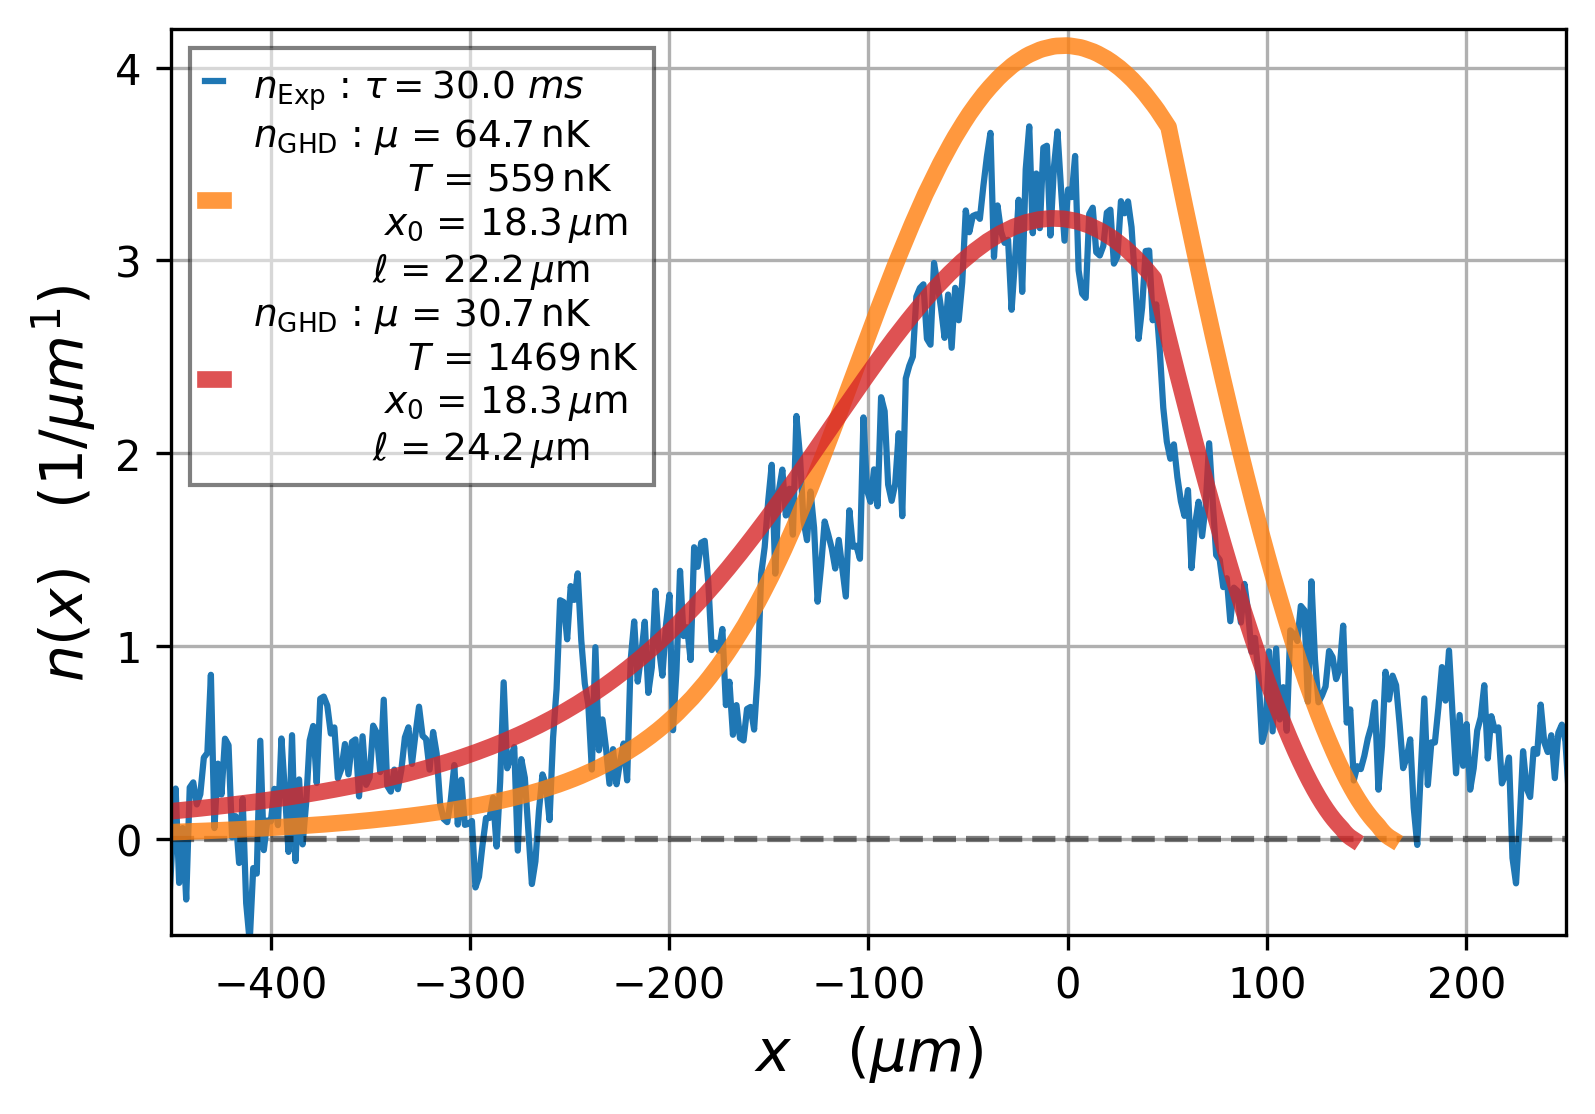
\includegraphics[width=\textwidth]{Figures/article_simul_expansion_1_09-02-2024}
        		\caption{}
        		\label{}
    		\end{subfigure}
    		\vspace{1em}
    		\begin{subfigure}[b]{1\textwidth}
				\centering
				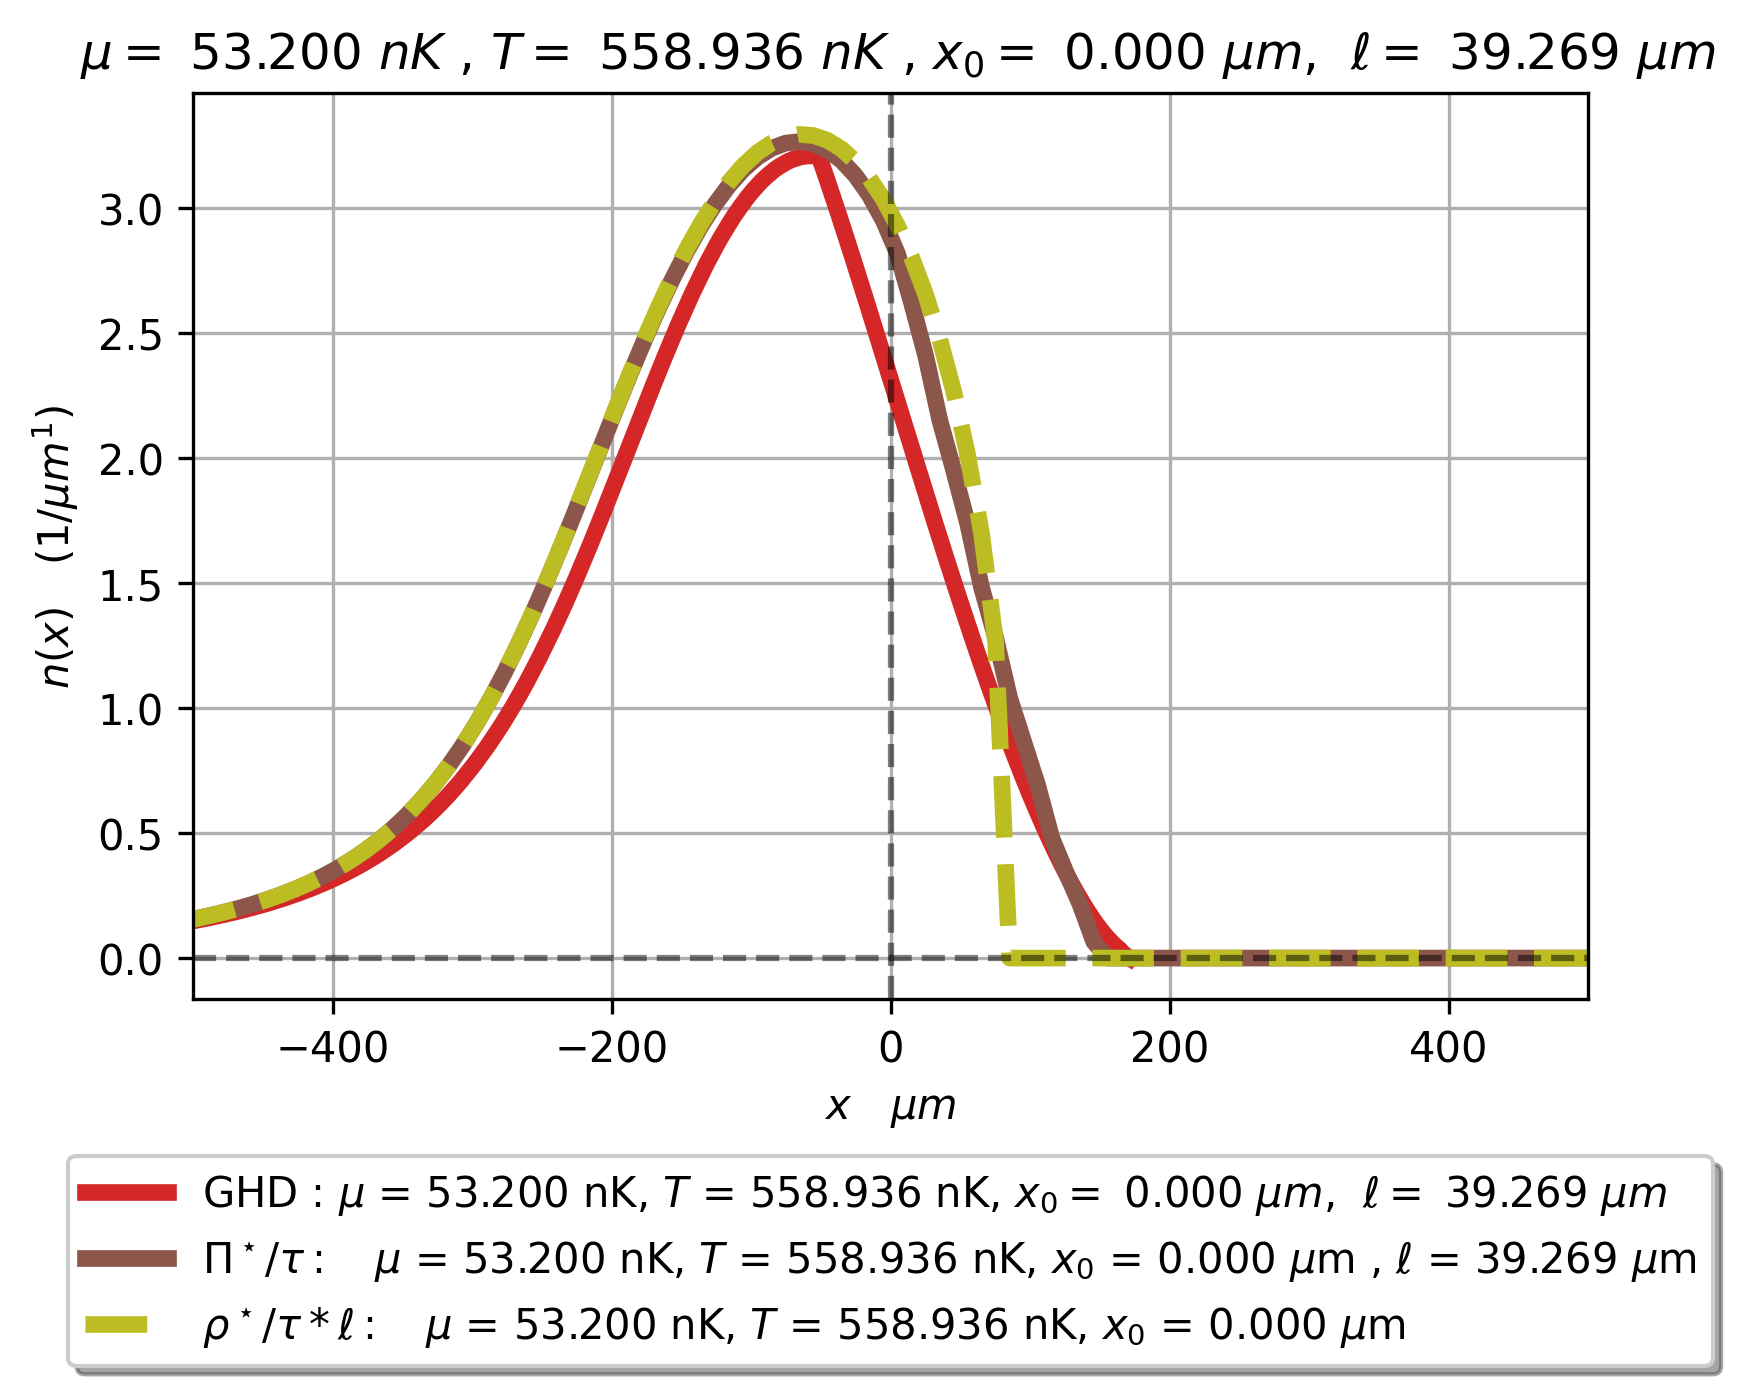
\includegraphics[width=0.48\textwidth]{Figures/article_distribution_09-02-2024}
				\caption{}
        		\label{}
			\end{subfigure}

				
		\end{figure}

		

	\section{Essancielle}
	
		\begin{figure}[H]
			\centering
			\begin{subfigure}[b]{1\textwidth}
        		\centering
       			 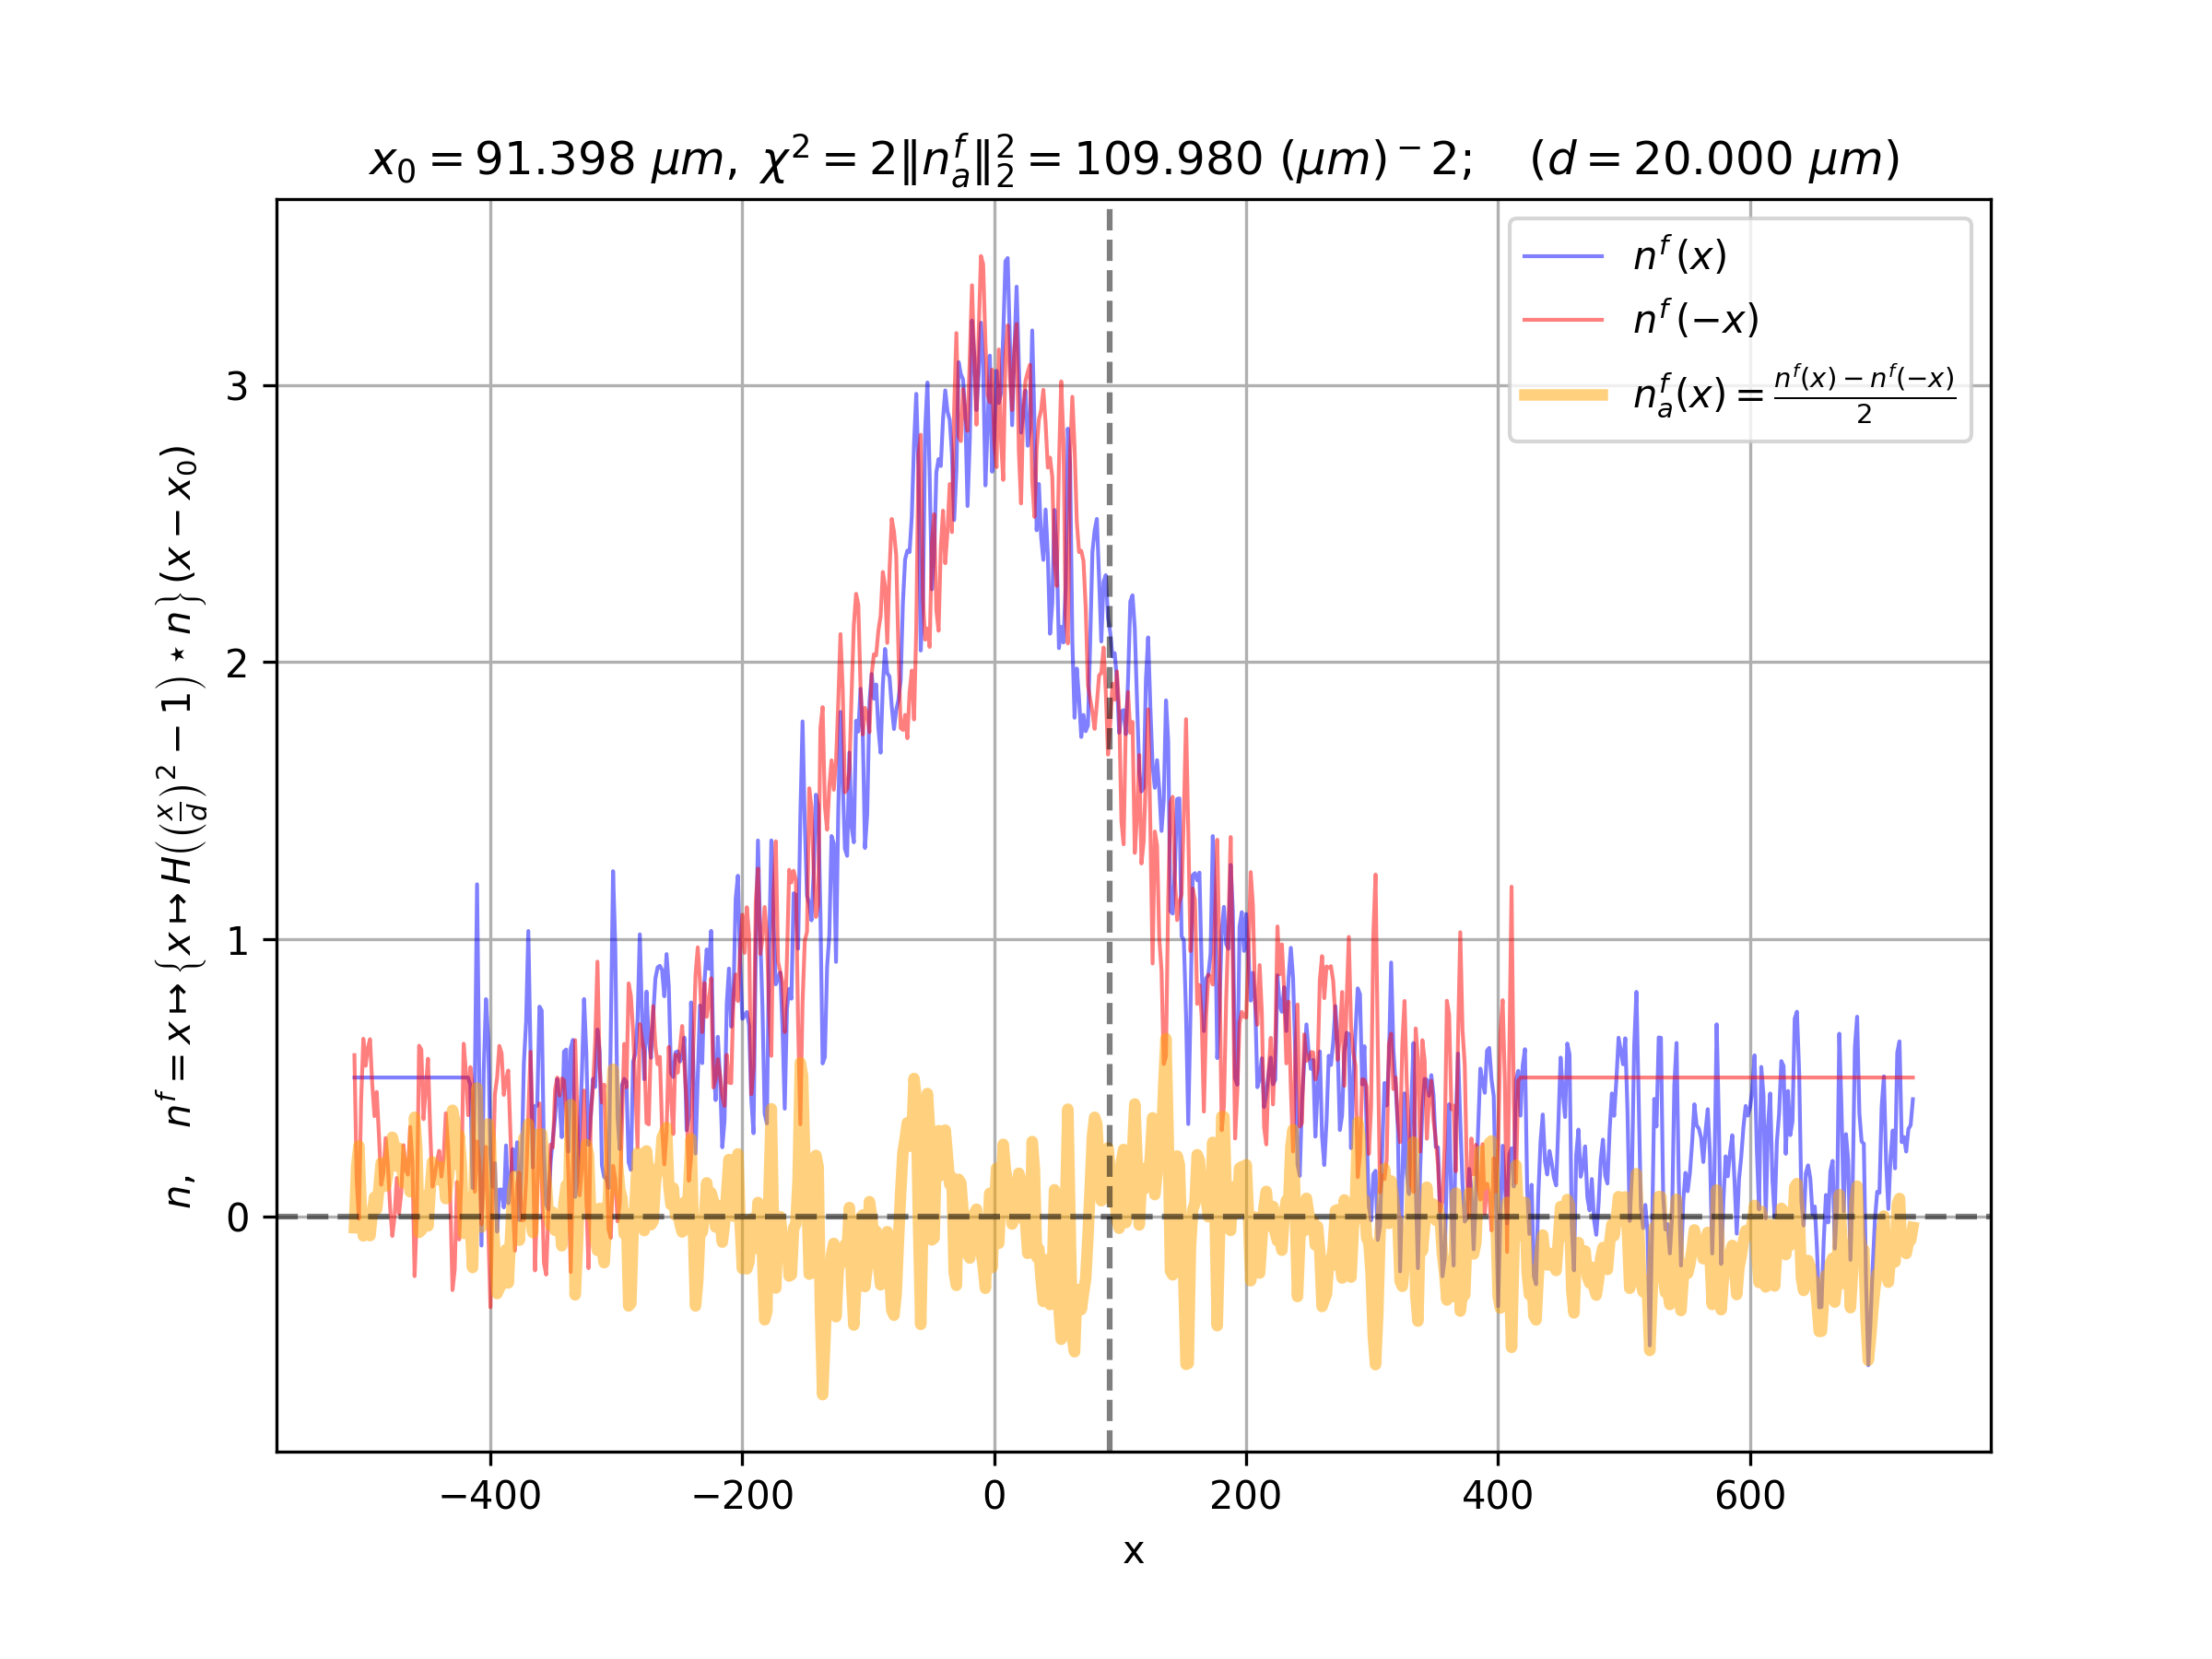
\includegraphics[width=0.48\textwidth]{Figures/asymetrie_09-02-2024}
       			 \caption{}
        		\label{}
   			 \end{subfigure}
   			 \vspace{1em}
   			 \begin{subfigure}[b]{0.48\textwidth}
   				 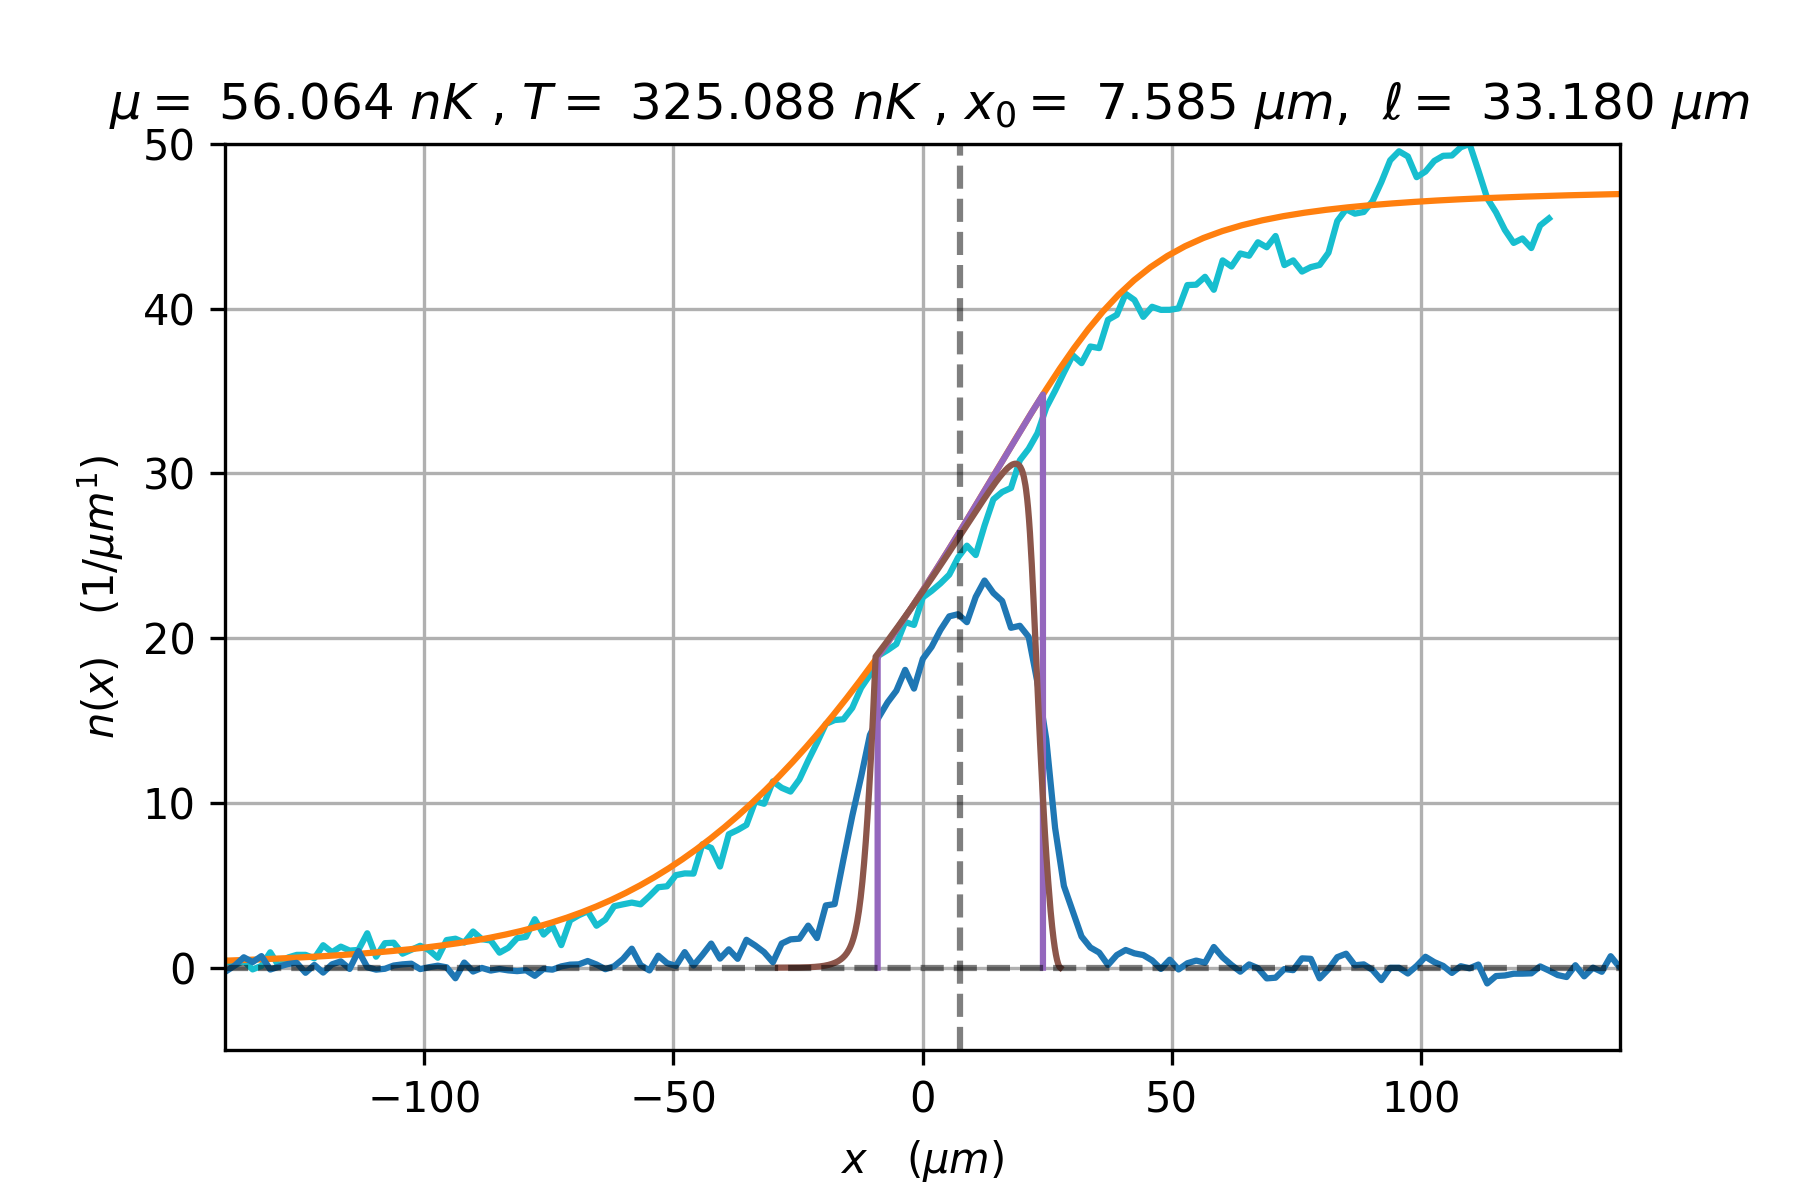
\includegraphics[width=\textwidth]{Figures/simul_deformation_1_09-02-2024}
        			\caption{}
        		\label{}
   			\end{subfigure}
    		\hfill
    		\begin{subfigure}[b]{0.48\textwidth}
        		\centering
        		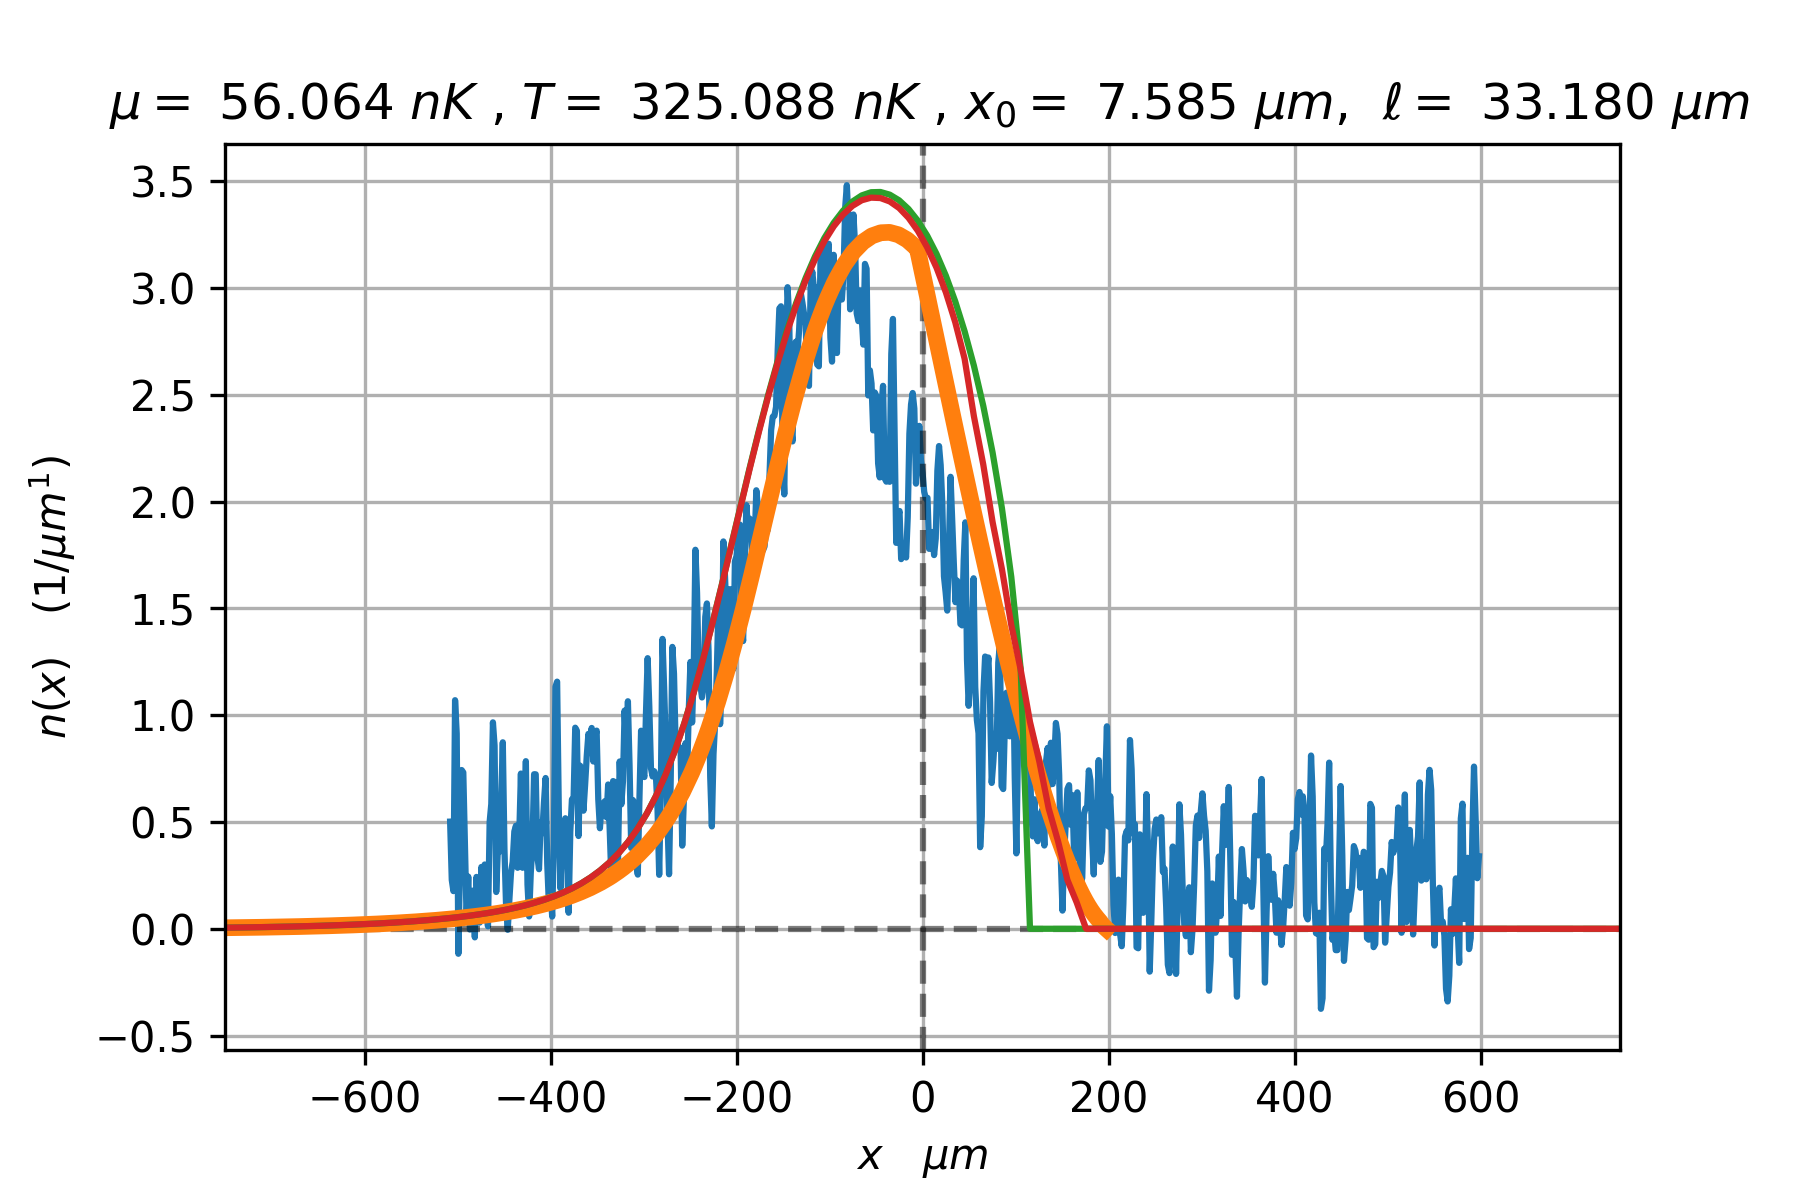
\includegraphics[width=\textwidth]{Figures/simul_expansion_1_09-02-2024}
        		\caption{}
        		\label{}
    		\end{subfigure}
    		\vspace{1em}
    		\begin{subfigure}[b]{0.48\textwidth}
   				 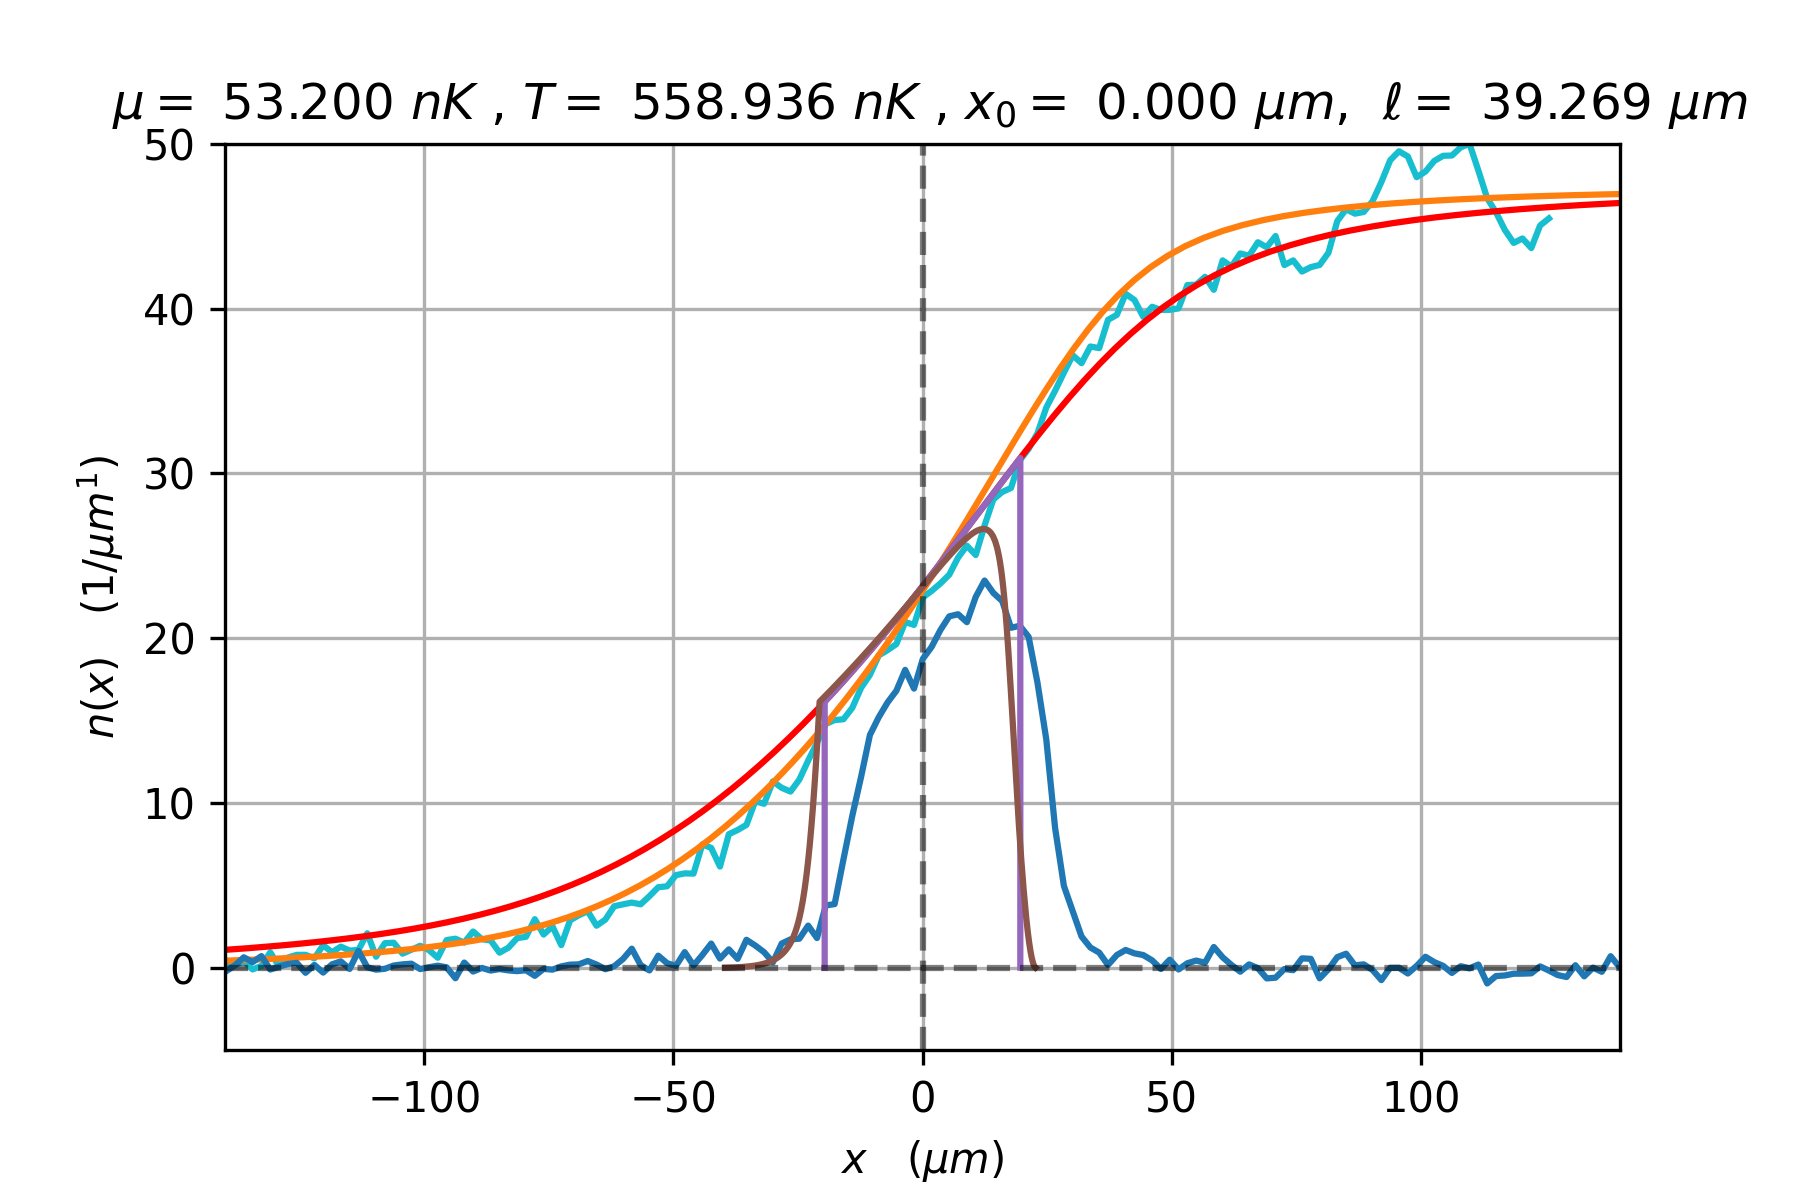
\includegraphics[width=\textwidth]{Figures/simul_deformation_4_09-02-2024}
        			\caption{}
        		\label{}
   			\end{subfigure}
    		\hfill
    		\begin{subfigure}[b]{0.48\textwidth}
        		\centering
        		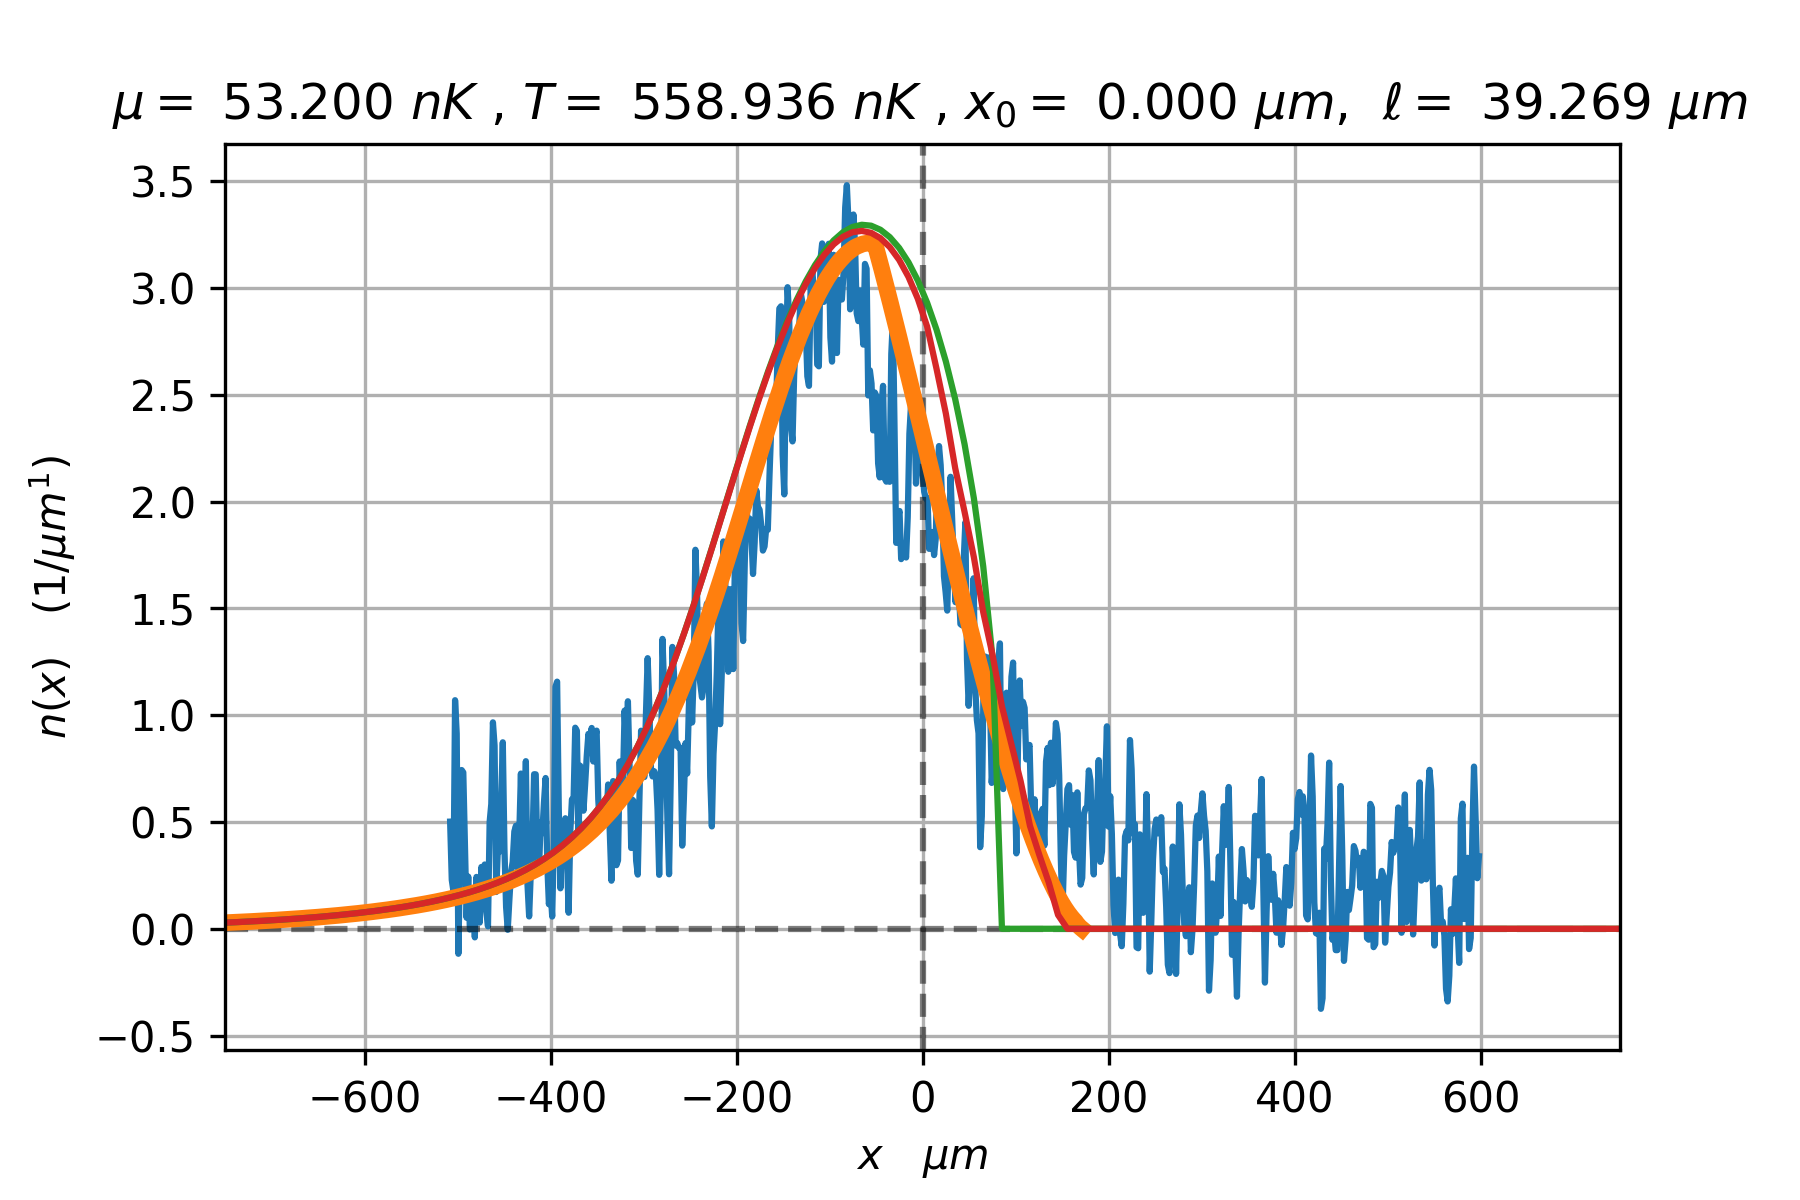
\includegraphics[width=\textwidth]{Figures/simul_expansion_4_09-02-2024}
        		\caption{}
        		\label{}
    		\end{subfigure}
    		
   			 \caption{Donnée du 09-02-2024}
   			 \label{}				
		\end{figure}
		
		\begin{figure}[H]
			\centering
			\begin{subfigure}[b]{1\textwidth}
        		\centering
       			 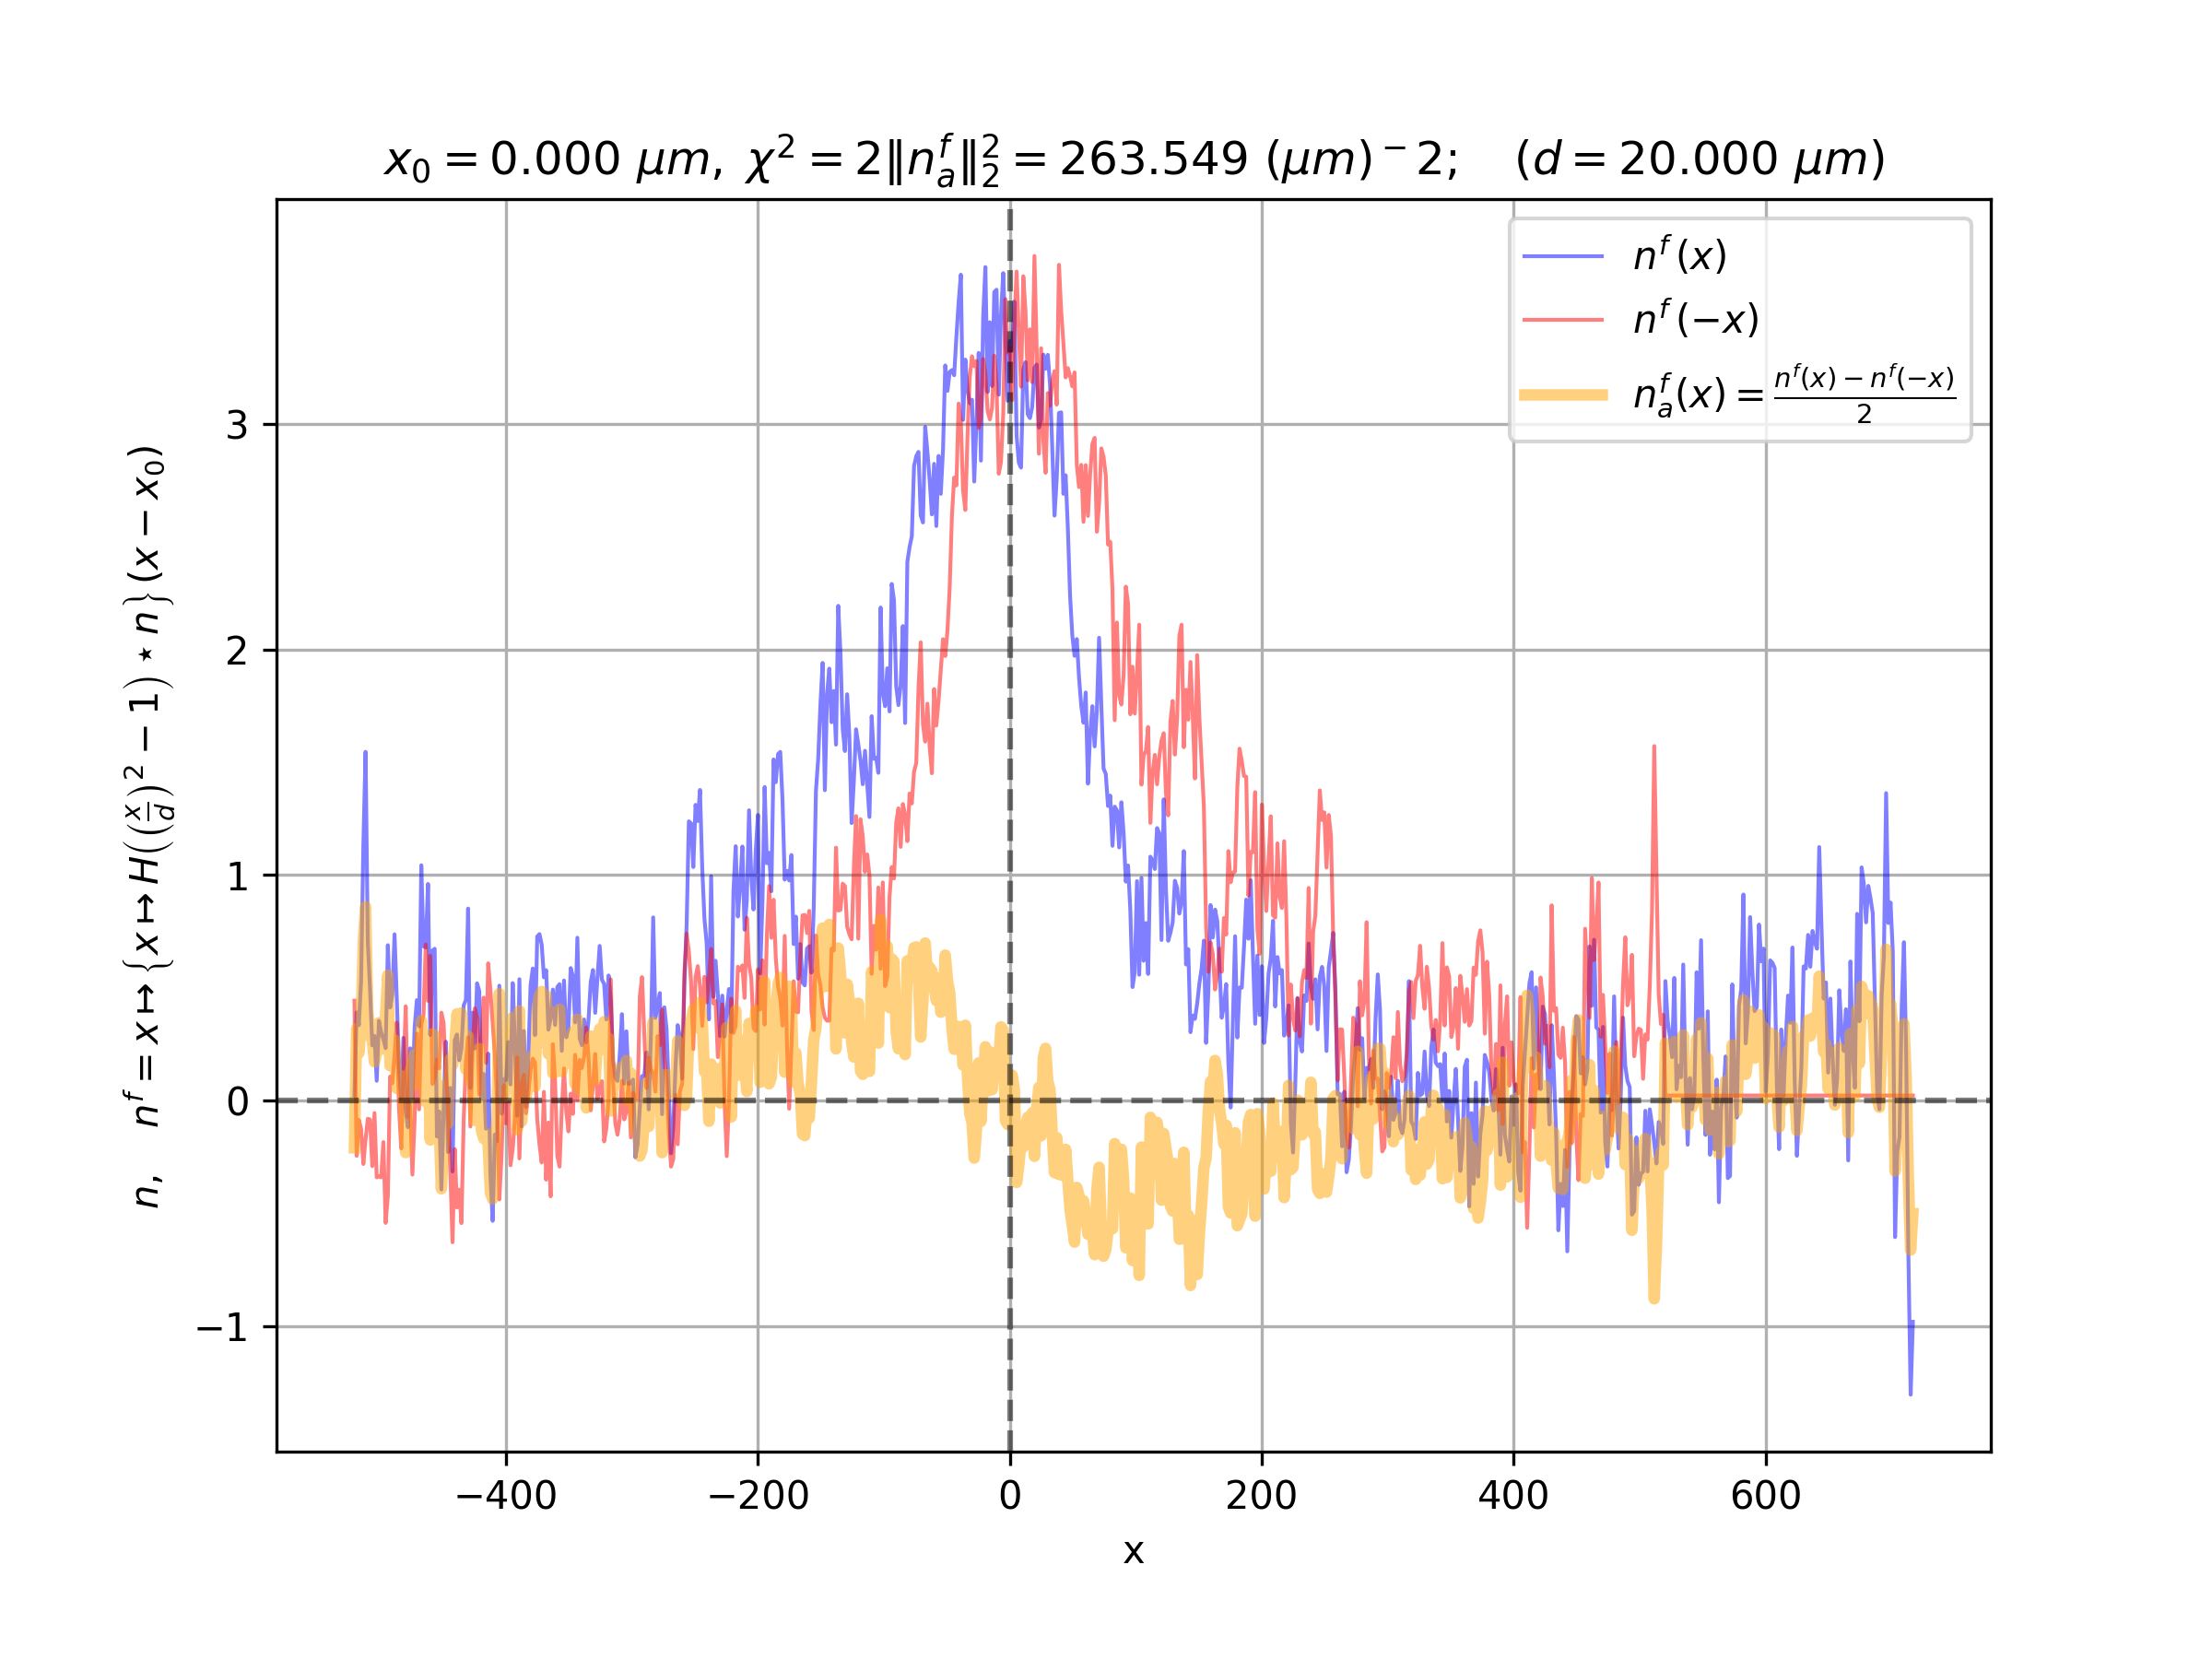
\includegraphics[width=0.48\textwidth]{Figures/asymetrie_24-04-2024}
       			 \caption{}
        		\label{}
   			 \end{subfigure}
   			 \vspace{1em}
   			 \begin{subfigure}[b]{0.48\textwidth}
   				 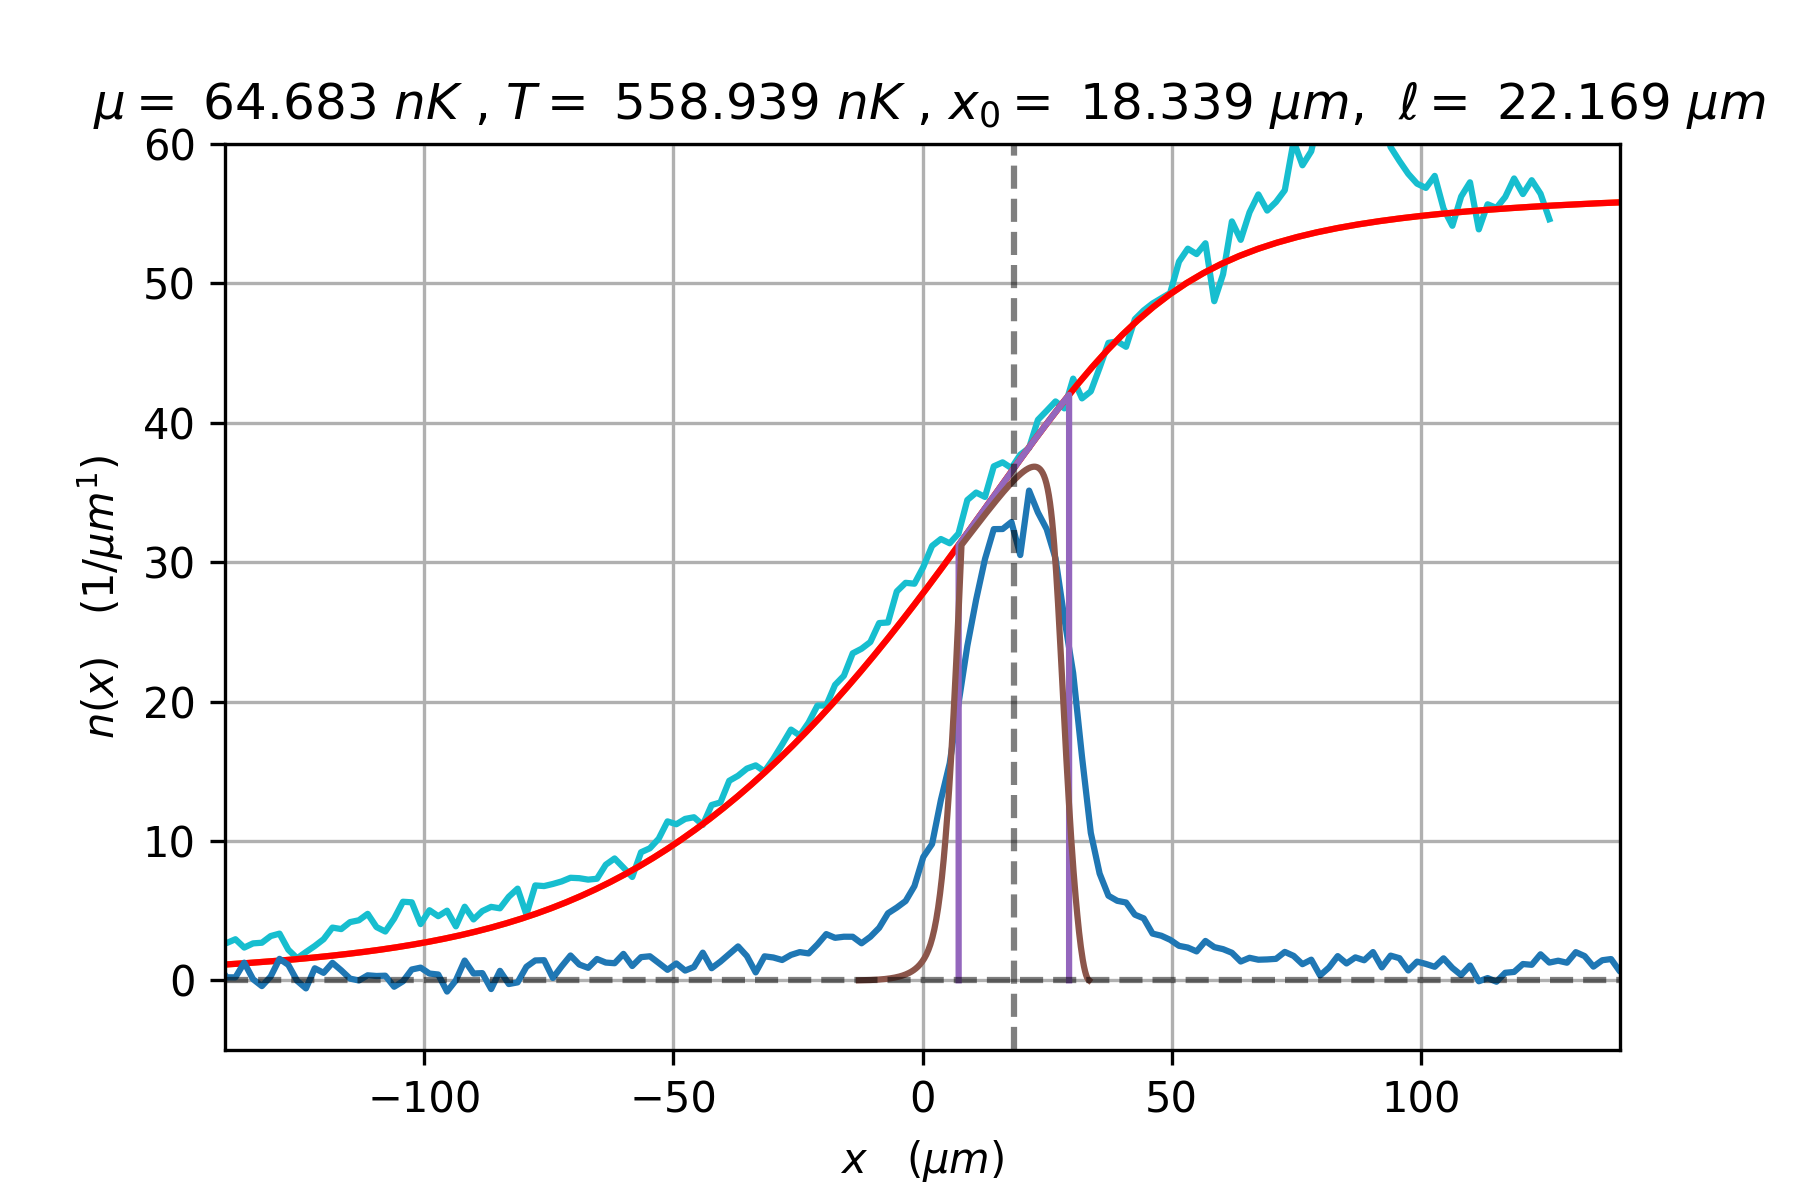
\includegraphics[width=\textwidth]{Figures/simul_deformation_1_24-04-2024}
        			\caption{}
        		\label{}
   			\end{subfigure}
    		\hfill
    		\begin{subfigure}[b]{0.48\textwidth}
        		\centering
        		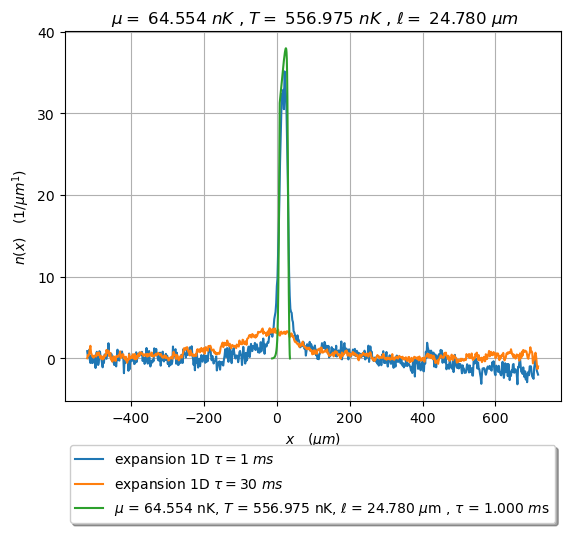
\includegraphics[width=\textwidth]{Figures/simul_expansion_1_24-04-2024}
        		\caption{}
        		\label{}
    		\end{subfigure}
    		\vspace{1em}
    		\begin{subfigure}[b]{0.48\textwidth}
   				 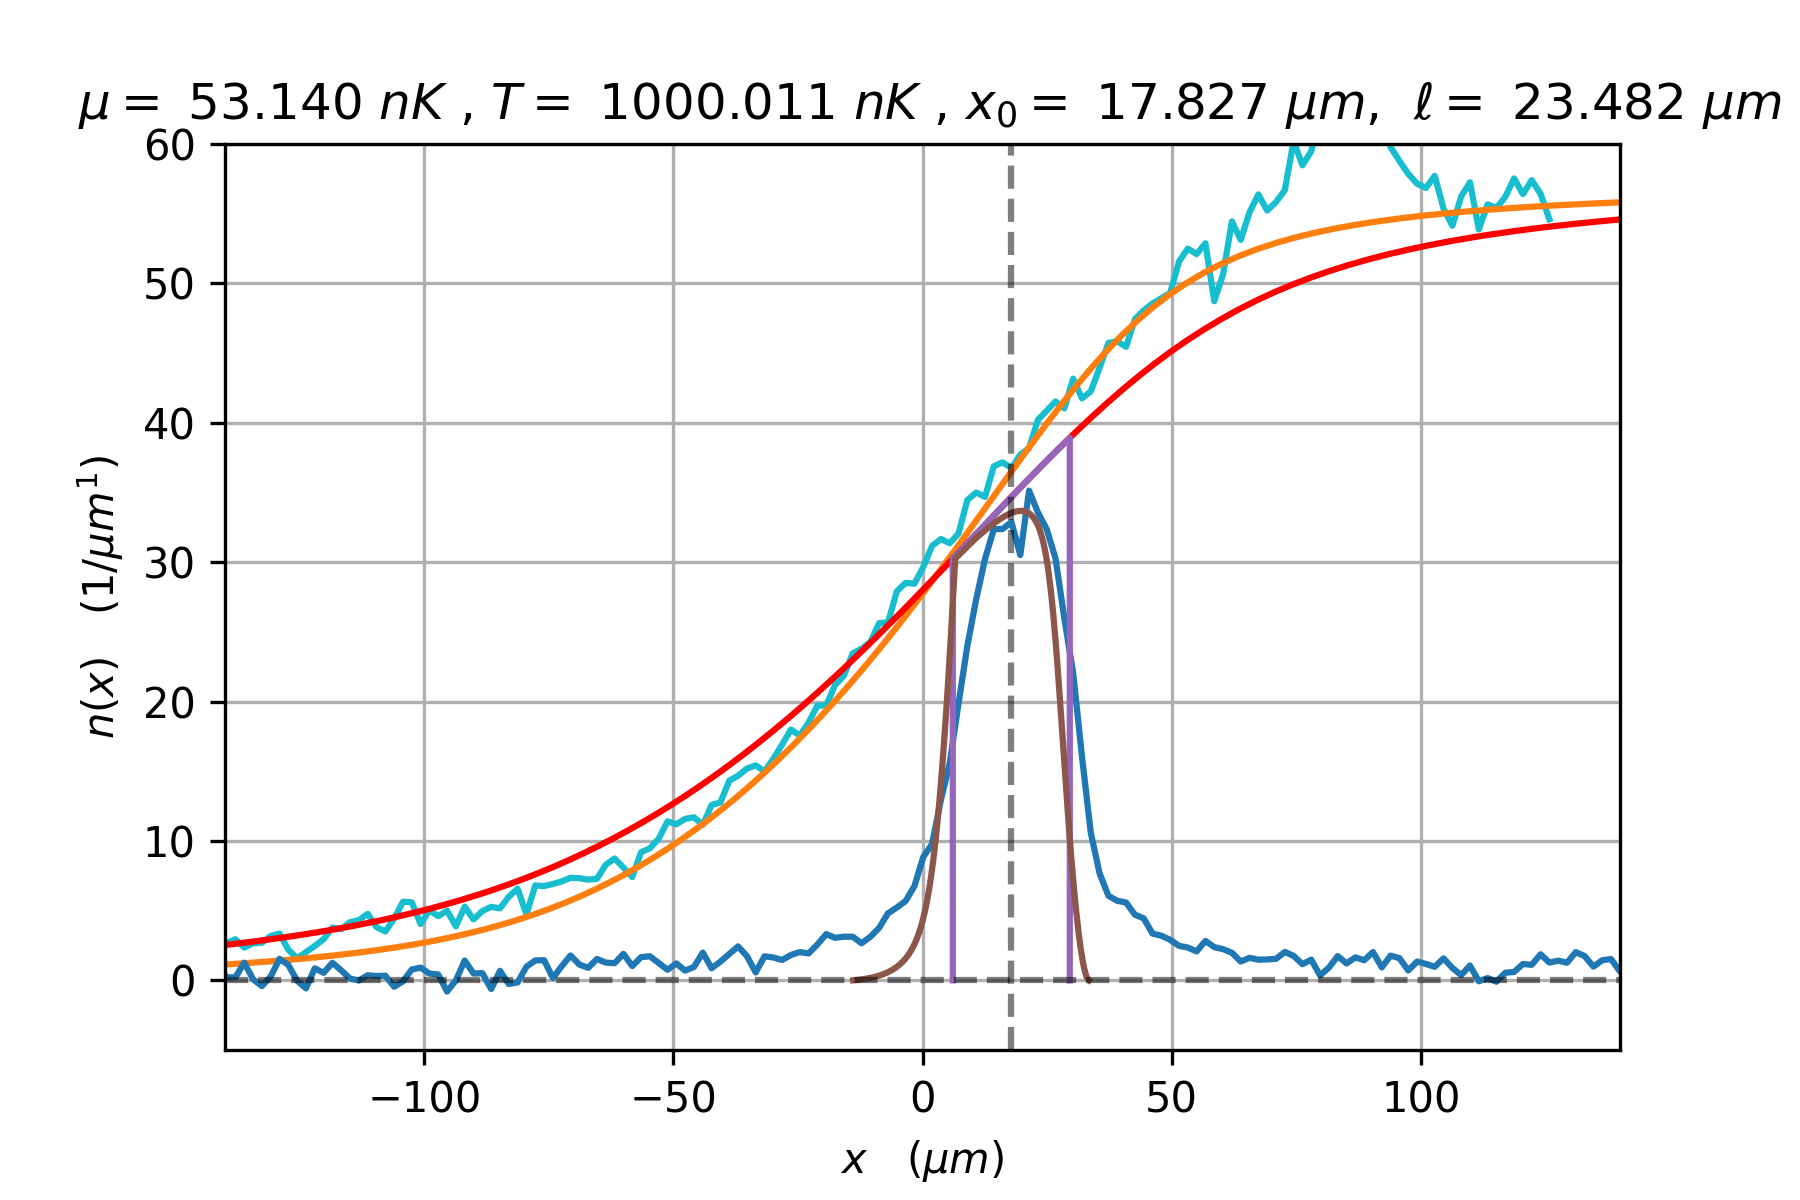
\includegraphics[width=\textwidth]{Figures/simul_deformation_5_24-04-2024}
        			\caption{}
        		\label{}
   			\end{subfigure}
    		\hfill
    		\begin{subfigure}[b]{0.48\textwidth}
        		\centering
        		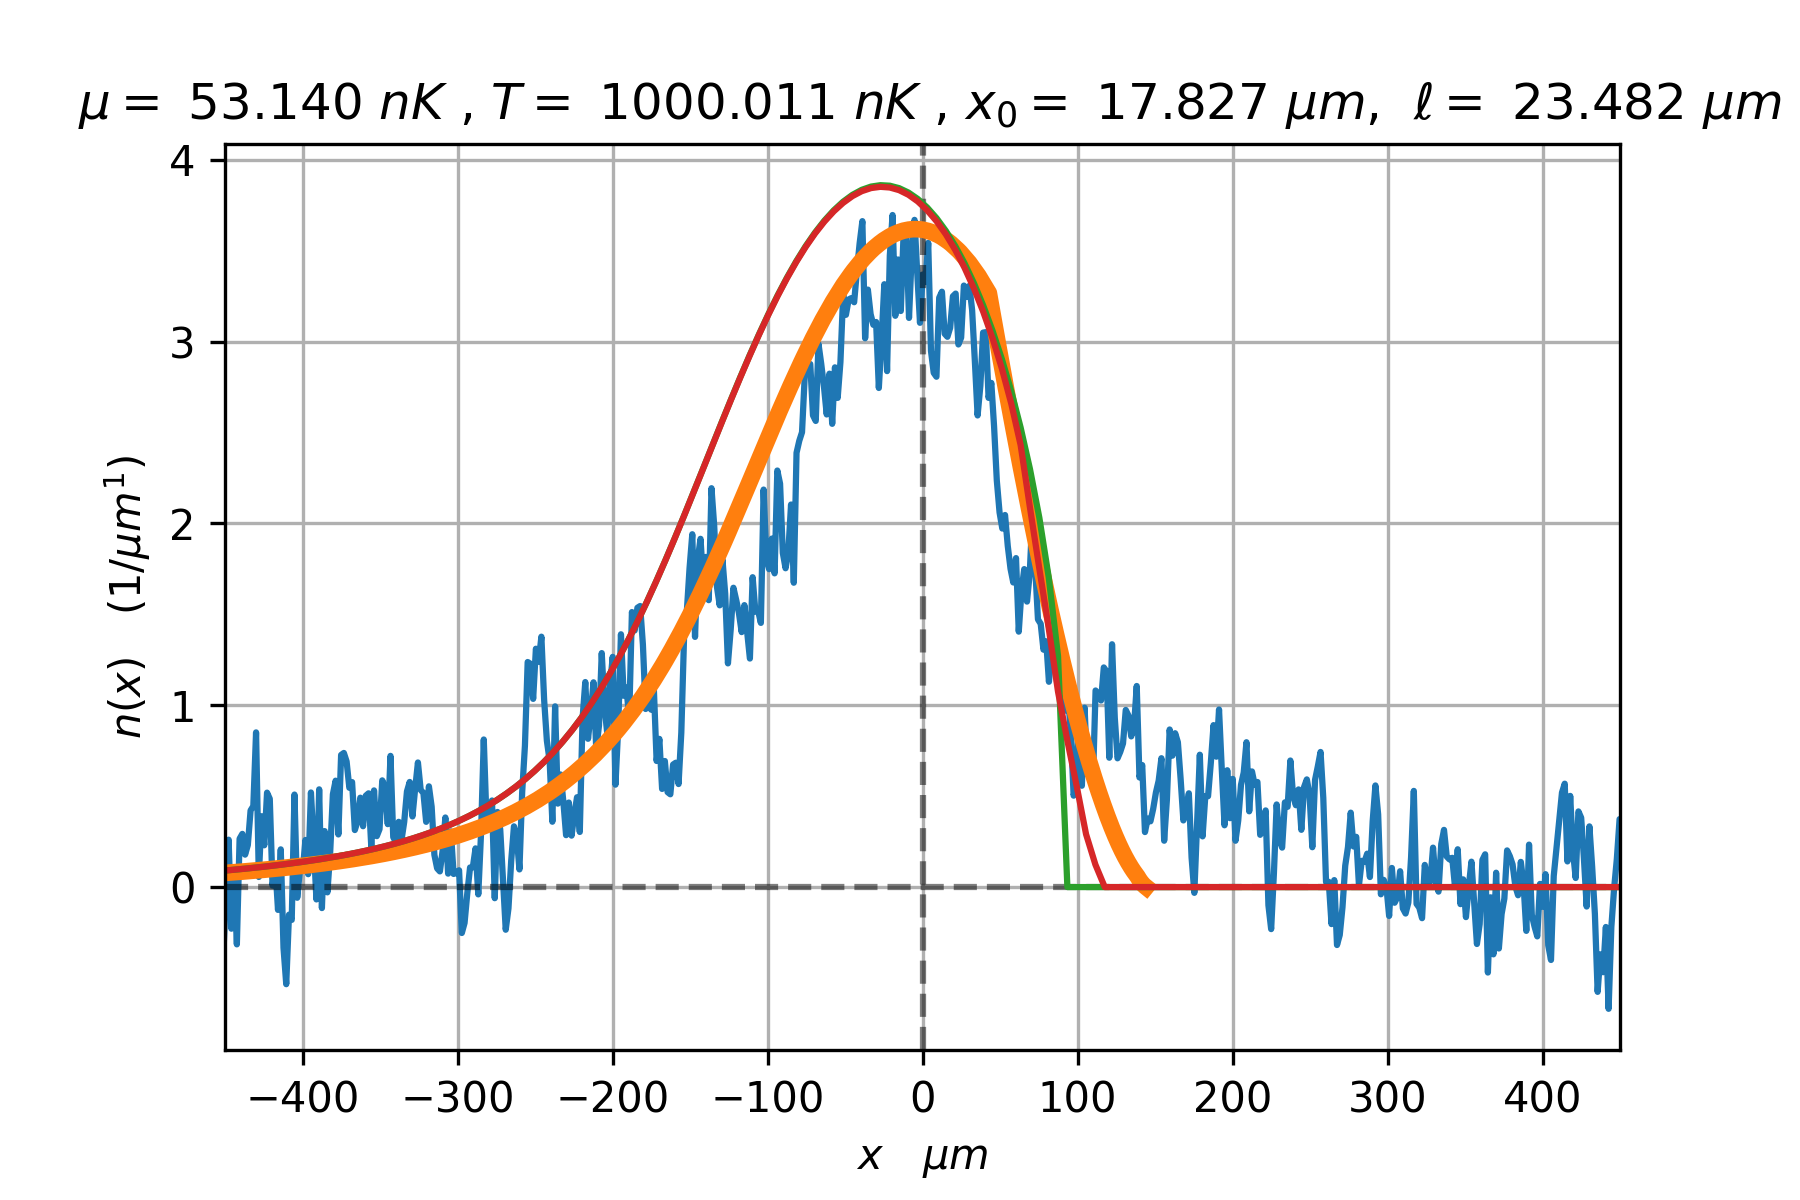
\includegraphics[width=\textwidth]{Figures/simul_expansion_5_24-04-2024}
        		\caption{}
        		\label{}
    		\end{subfigure}
    		
   			 \caption{Donnée du 24-04-2024}
   			 \label{}				
		\end{figure}


	
	\begin{figure}[H]
	\centering

    
    \begin{subfigure}[b]{0.48\textwidth}
        \centering
        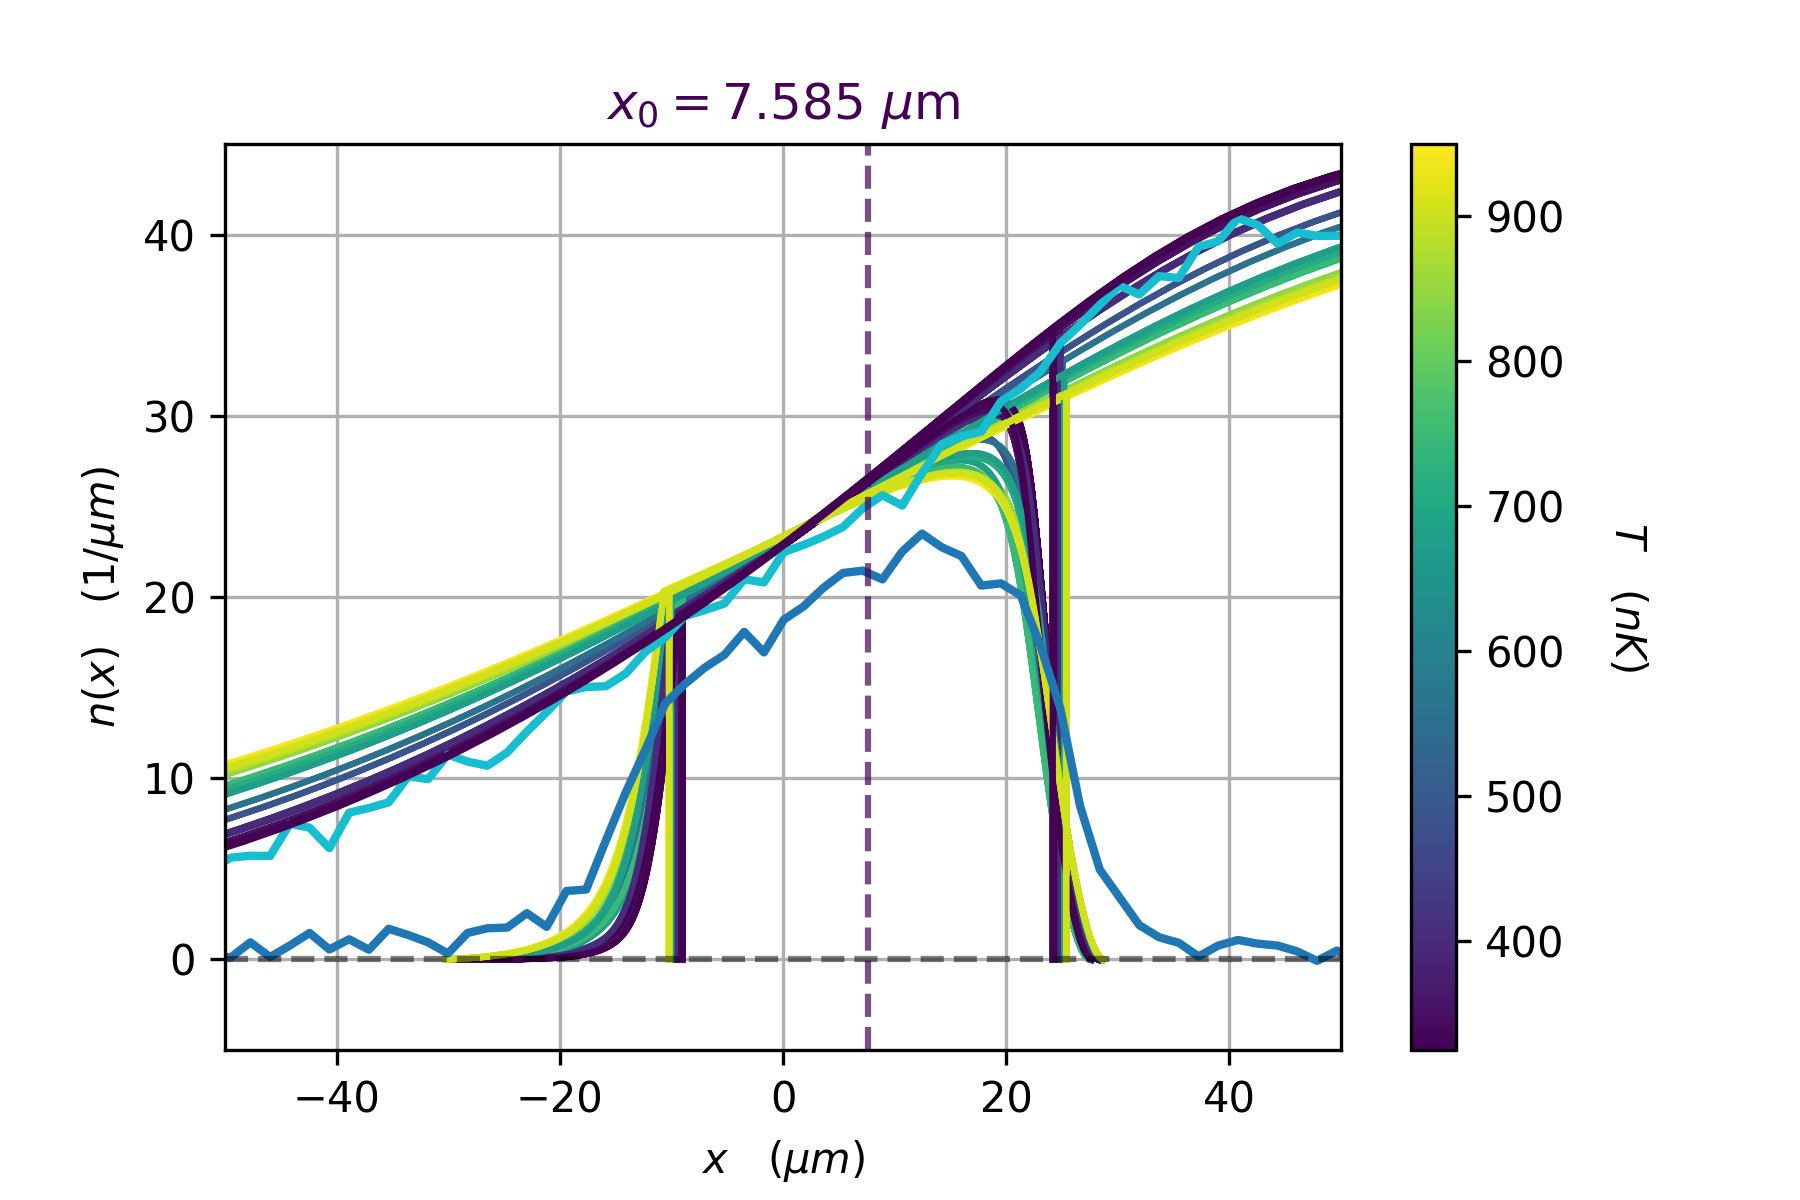
\includegraphics[width=\textwidth]{Figures/simul_deformation_T_09-02-2024}
        \caption{}
        \label{}
    \end{subfigure}
    \hfill
    \begin{subfigure}[b]{0.48\textwidth}
        \centering
        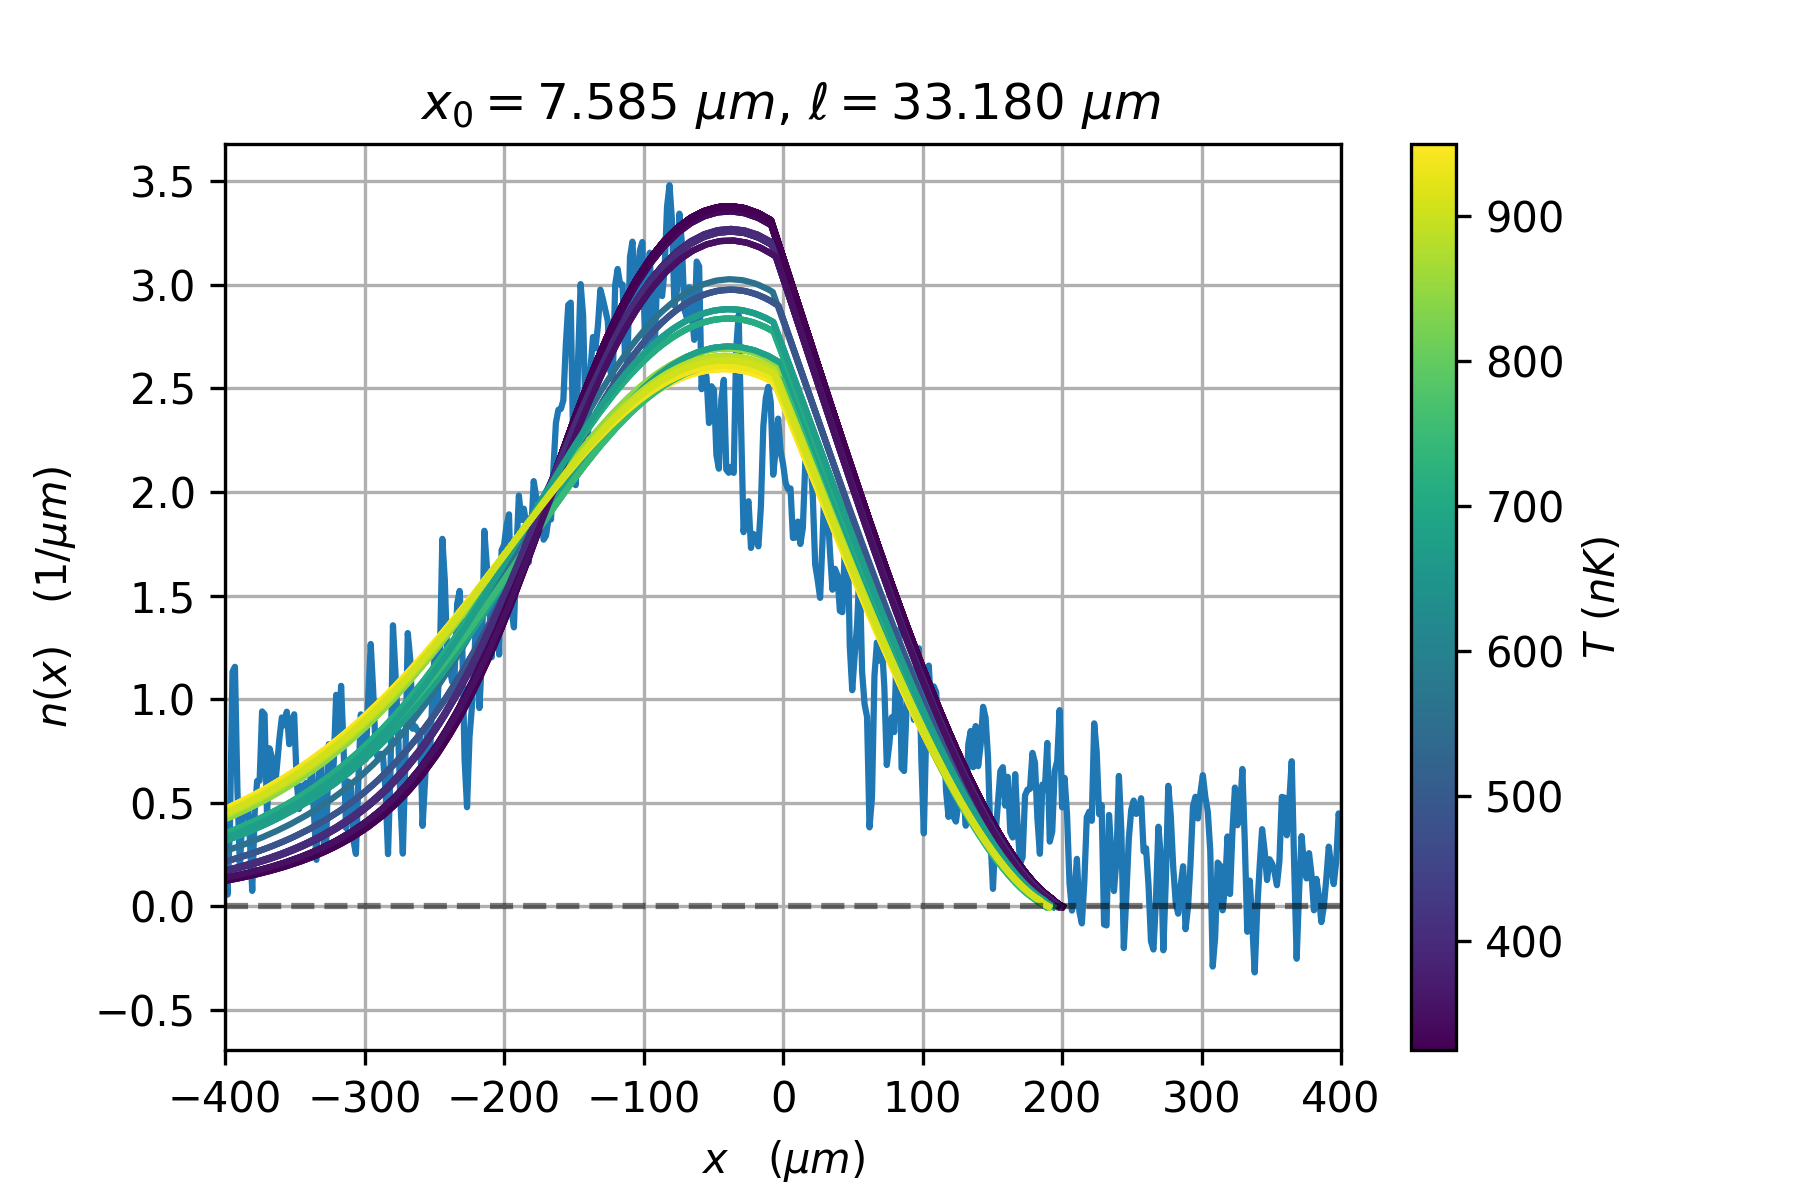
\includegraphics[width=\textwidth]{Figures/simul_expansion_T_09-02-2024}
        \caption{}
        \label{}
    \end{subfigure}
    \vspace{1em}
    \begin{subfigure}[b]{0.48\textwidth}
        \centering
        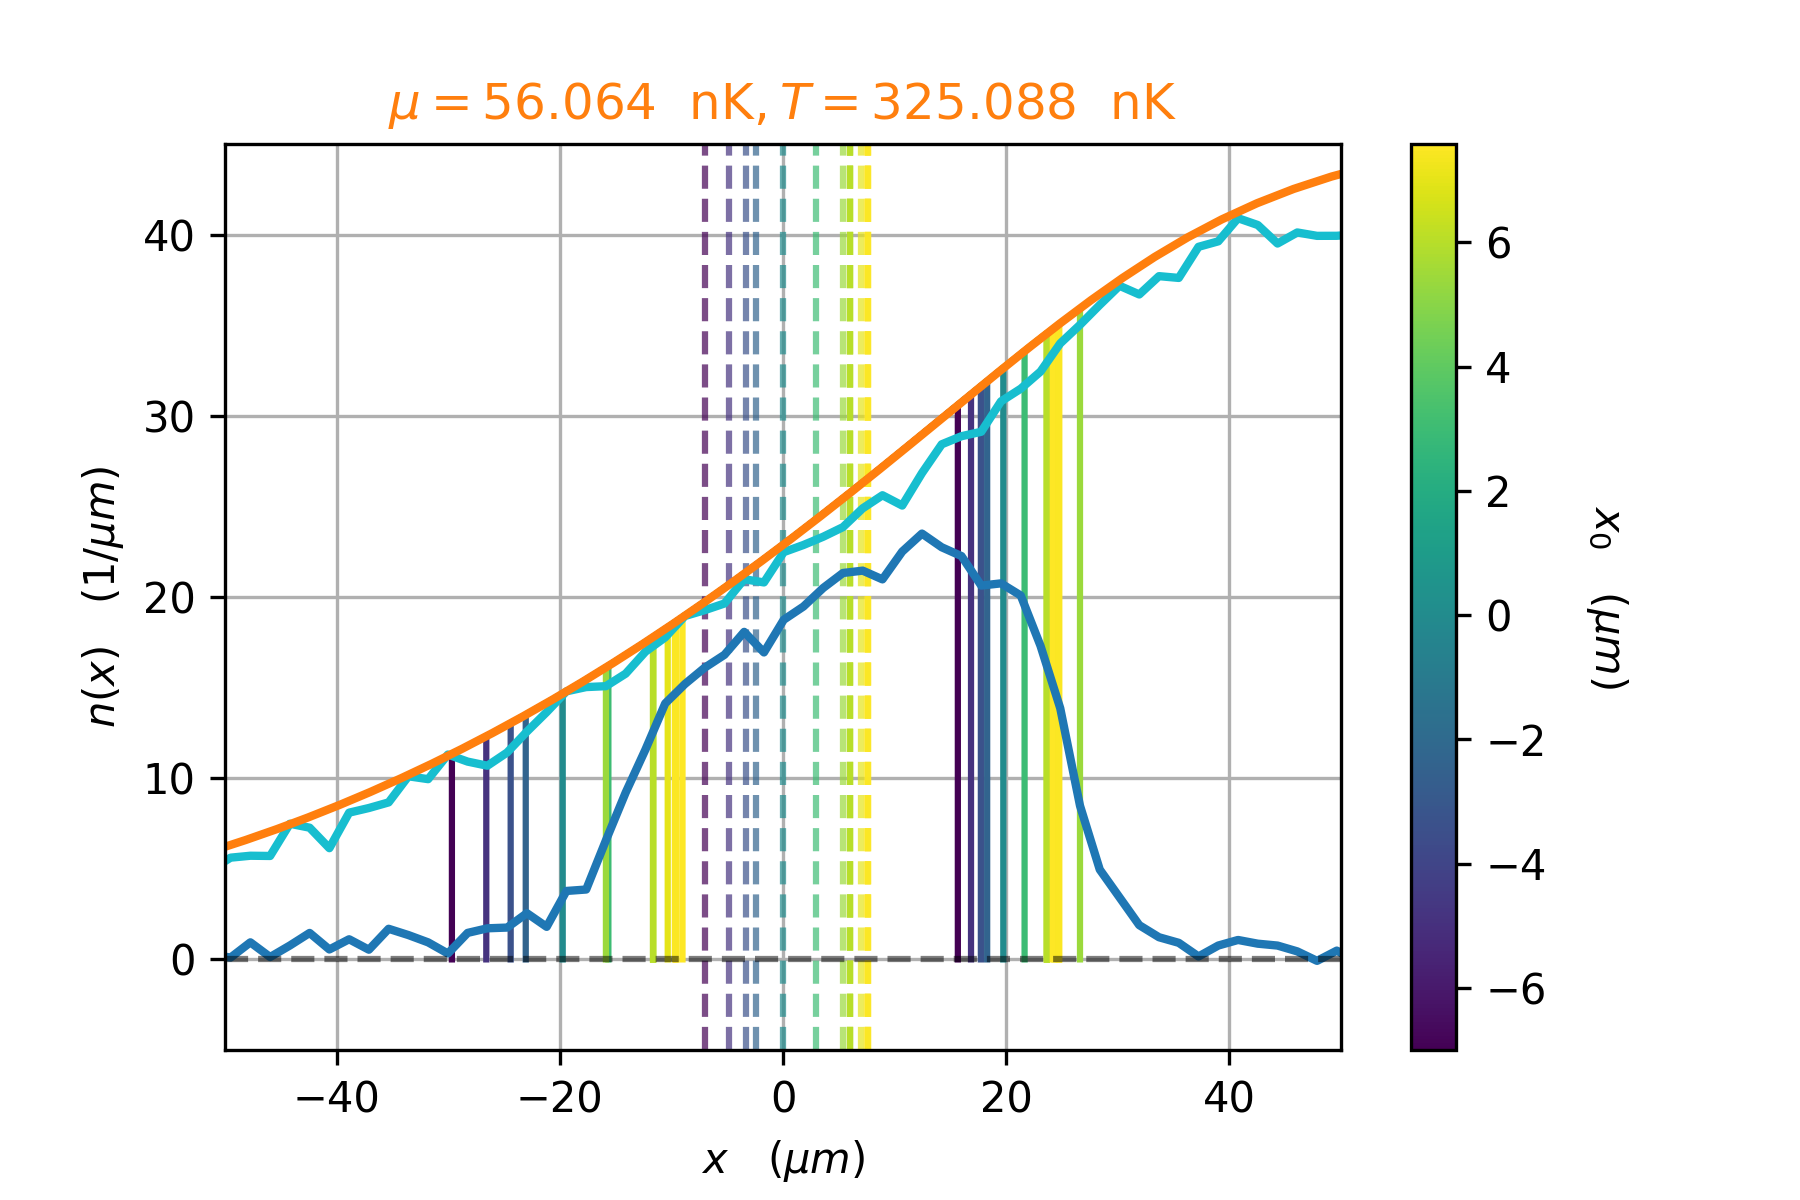
\includegraphics[width=\textwidth]{Figures/simul_deformation_x0_09-02-2024}
        \caption{}
        \label{}
    \end{subfigure}
    \hfill
    \begin{subfigure}[b]{0.48\textwidth}
        \centering
        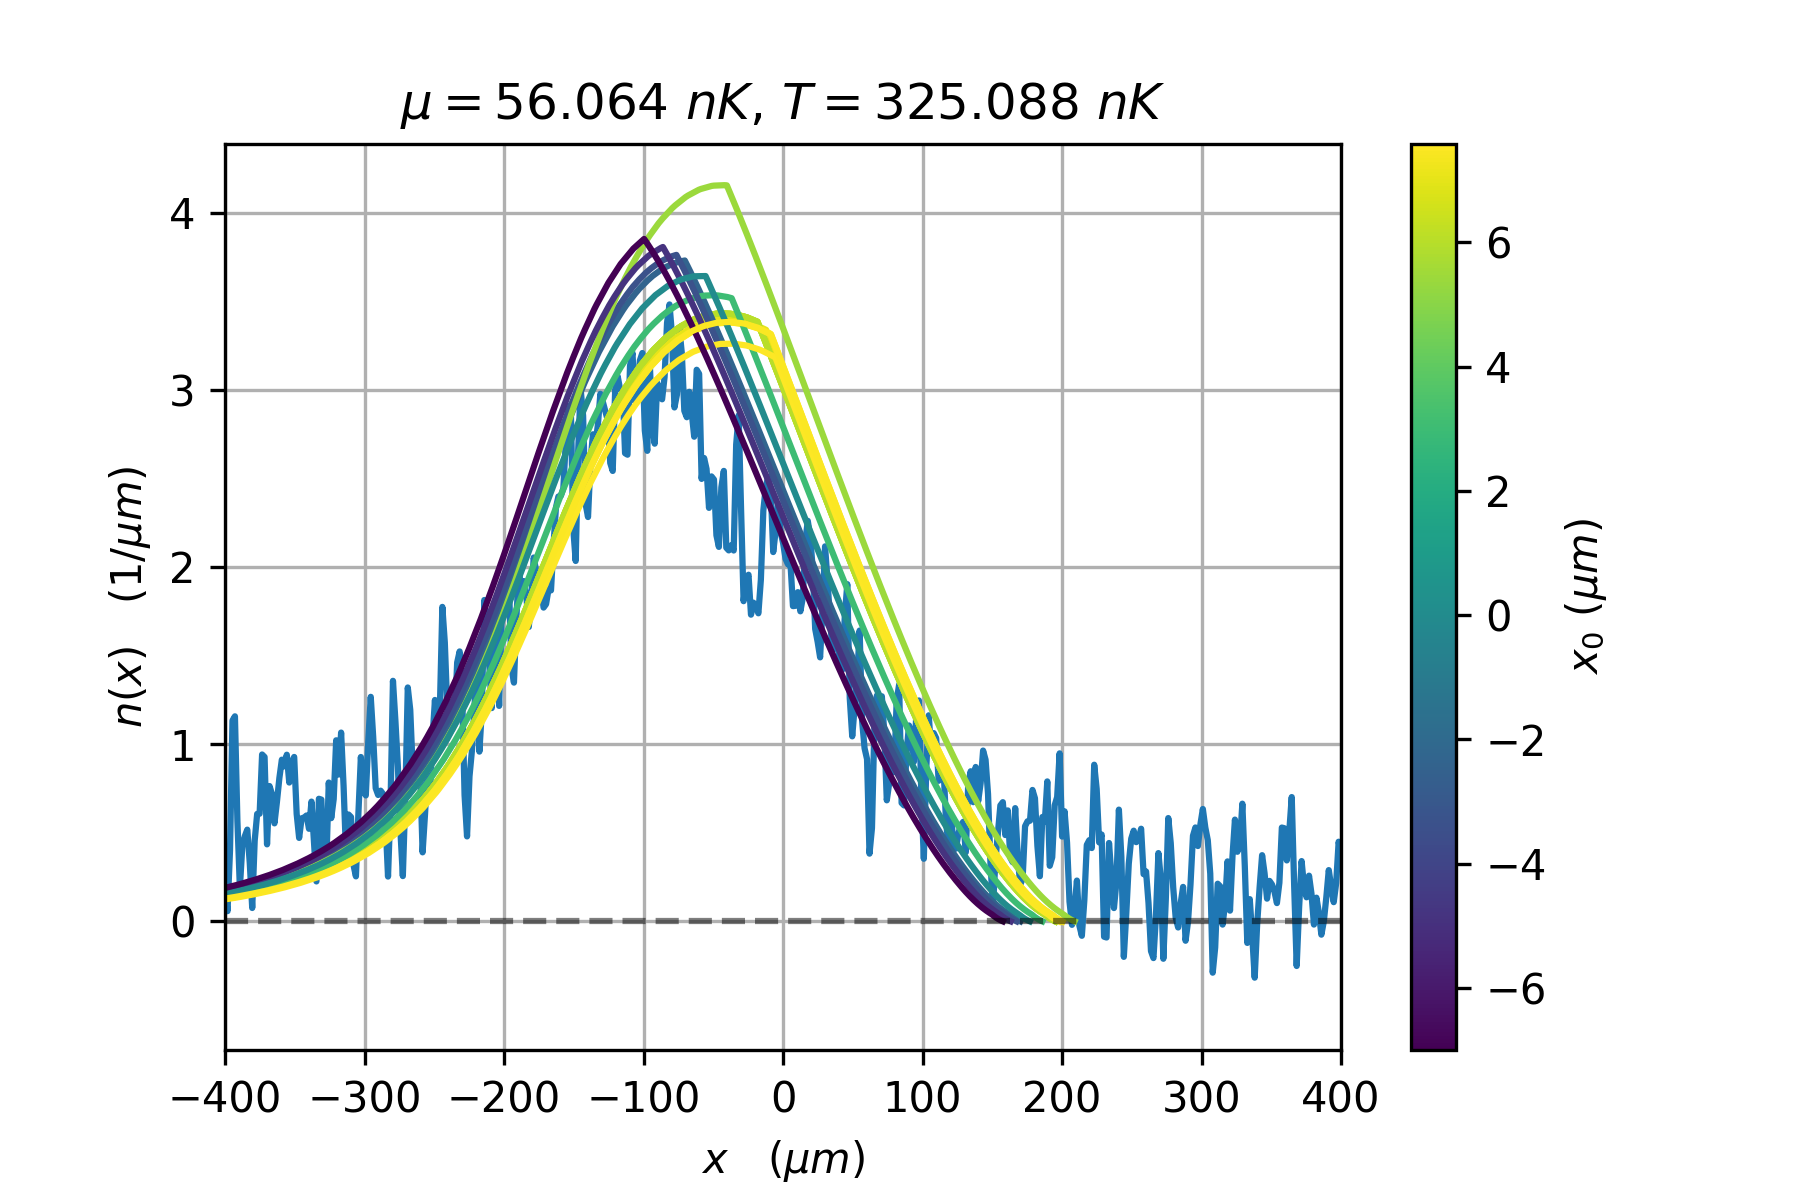
\includegraphics[width=\textwidth]{Figures/simul_expansion_x0_09-02-2024}
        \caption{}
        \label{}
    \end{subfigure}
    \vspace{1em}
%    \begin{subfigure}[b]{0.48\textwidth}
%        \centering
%        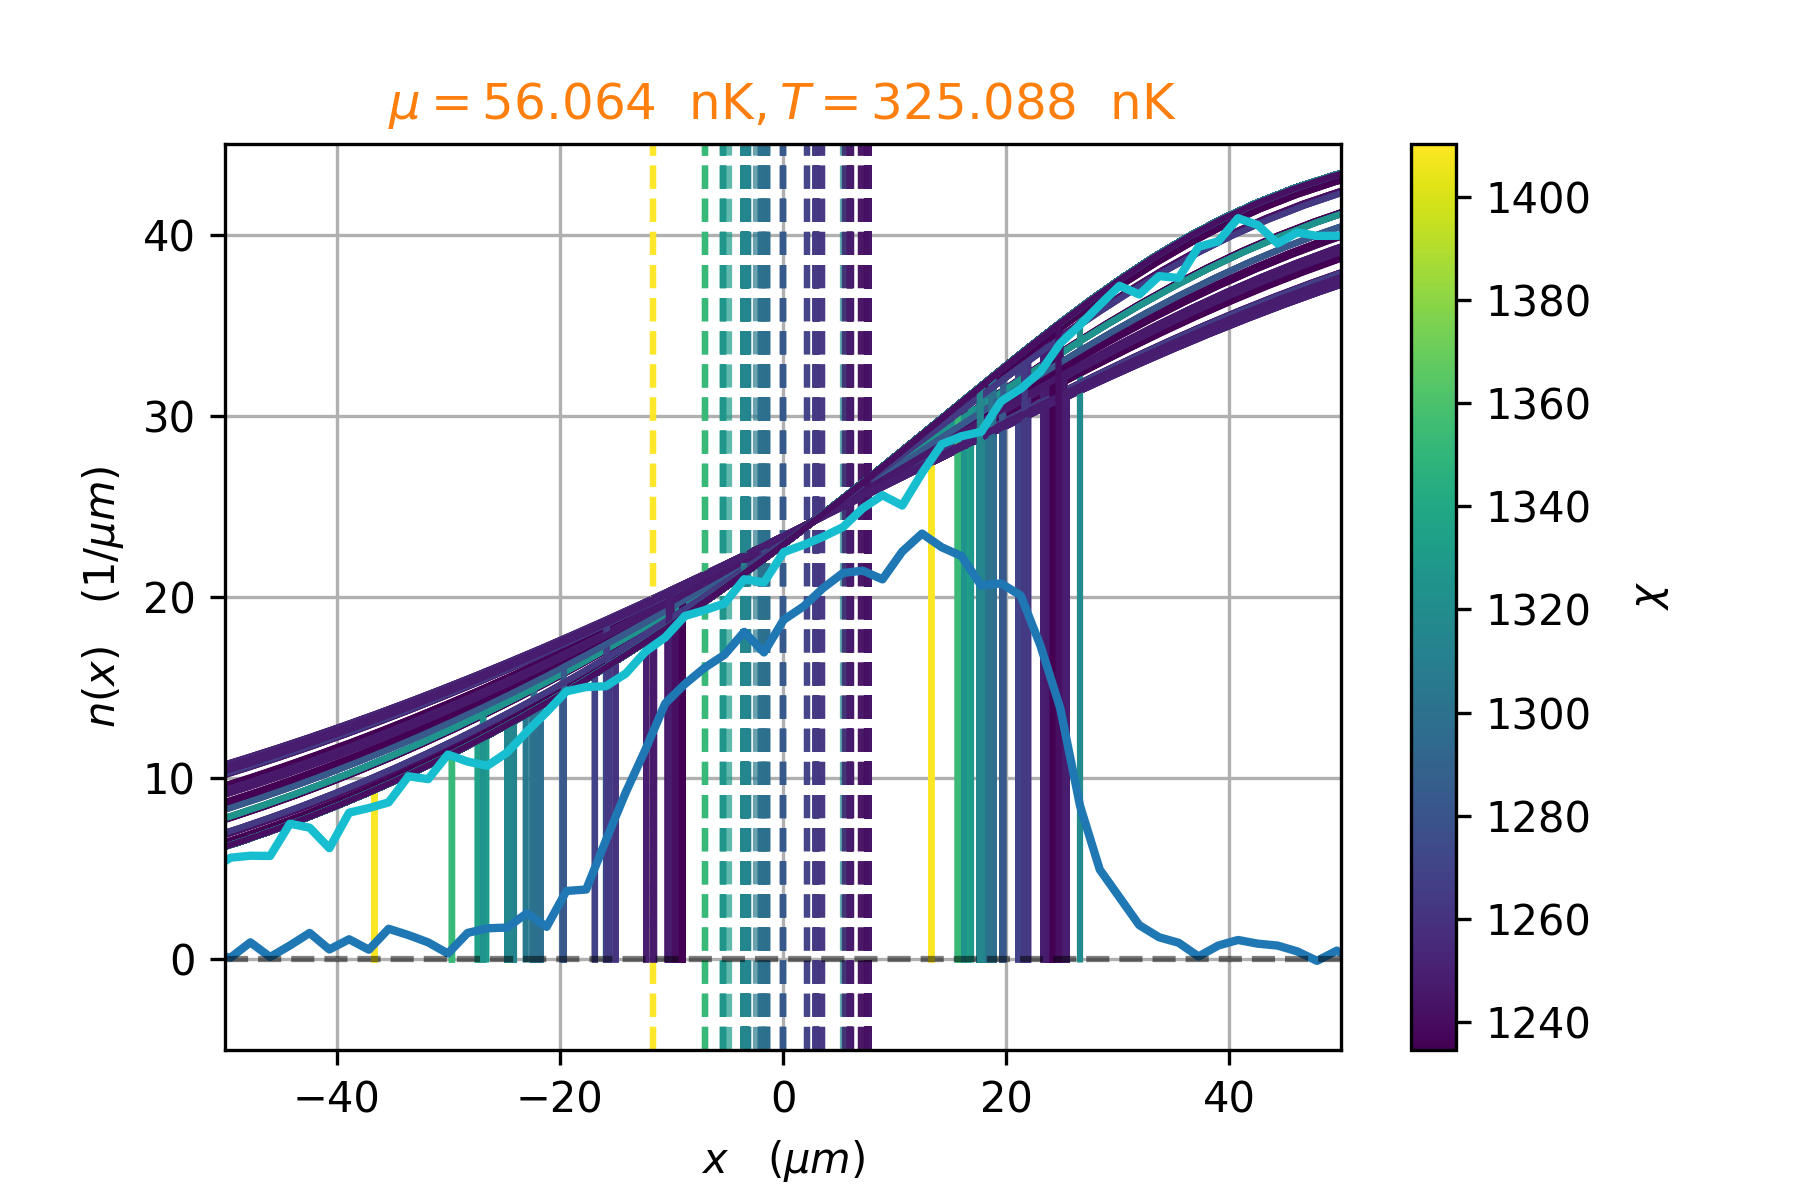
\includegraphics[width=\textwidth]{Figures/simul_deformation_T-x0_09-02-2024}
%        \caption{}
%        \label{}
%    \end{subfigure}
%    \hfill
%    \begin{subfigure}[b]{0.48\textwidth}
%        \centering
%        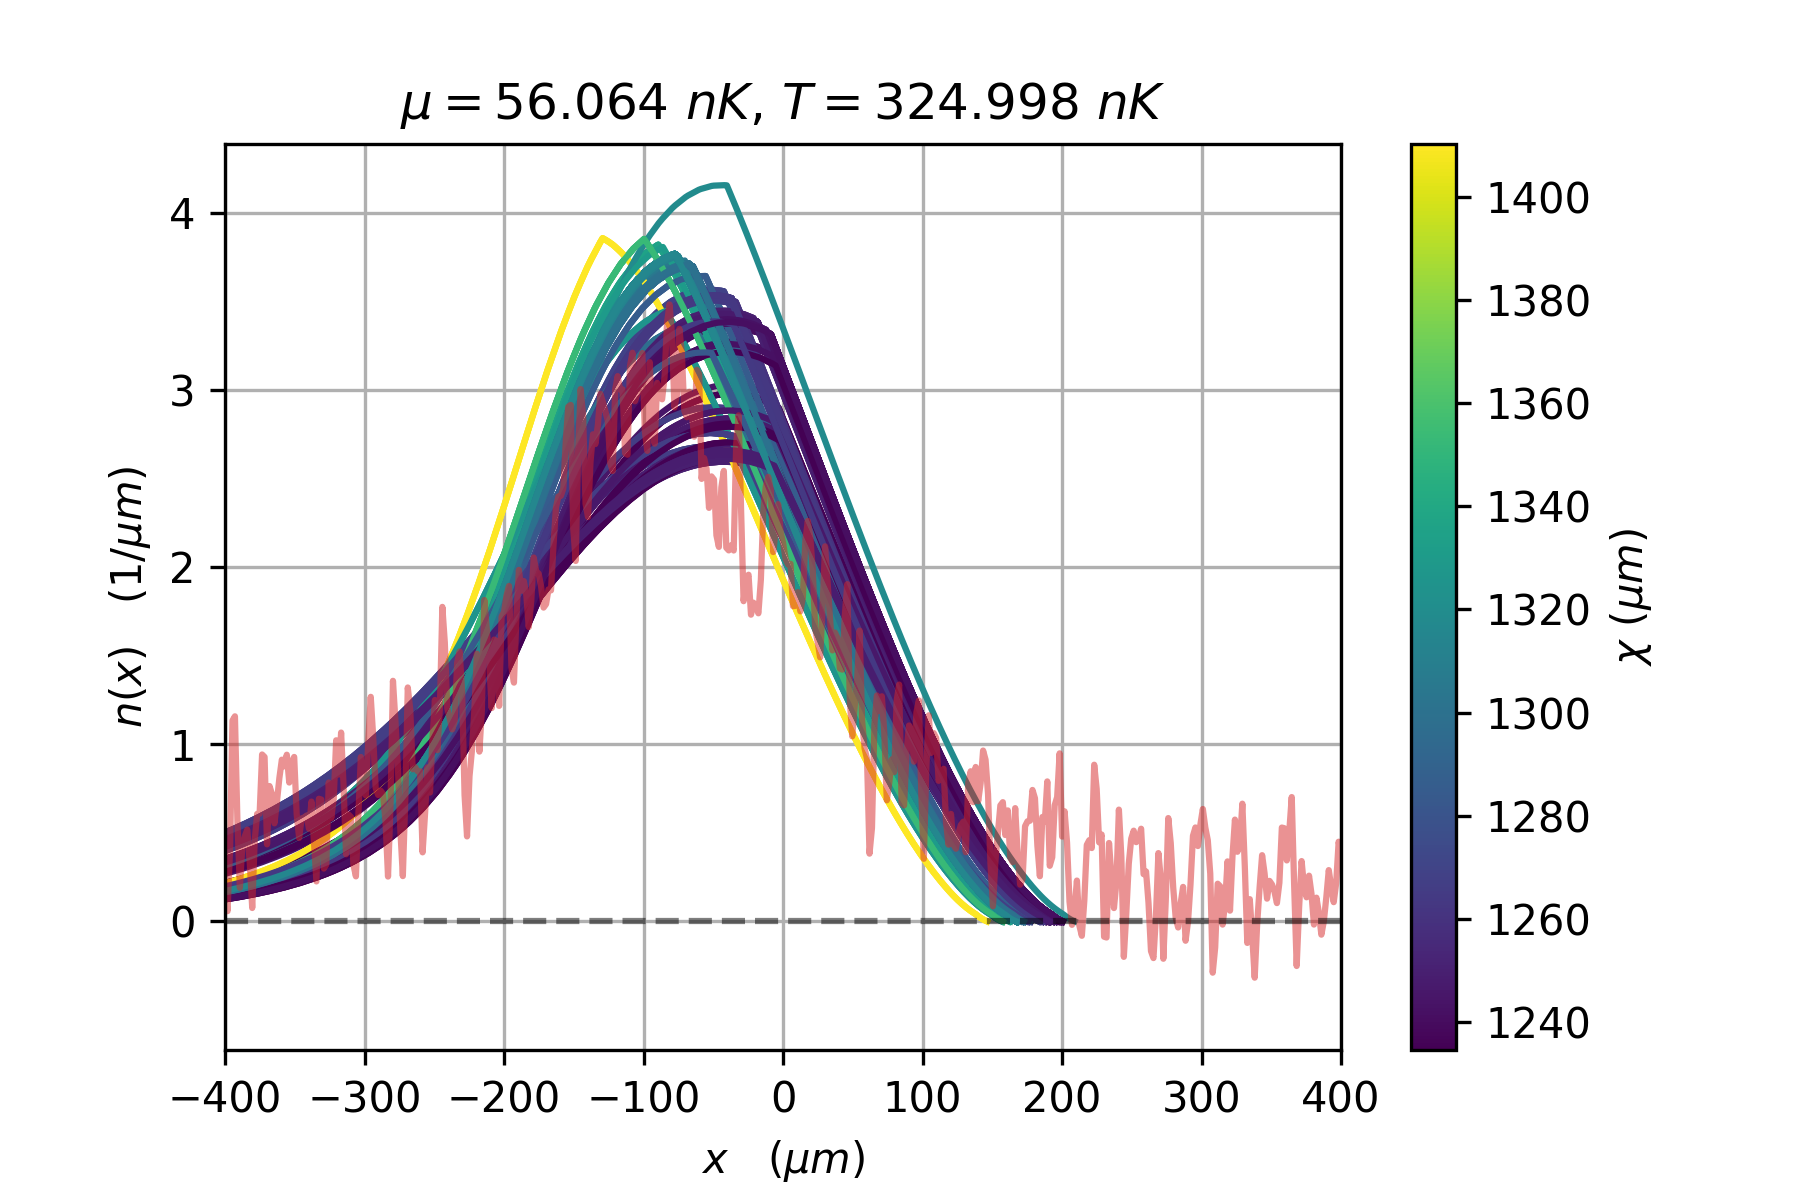
\includegraphics[width=\textwidth]{Figures/simul_expansion_T-x0_09-02-2024}
%        \caption{}
%        \label{}
%    \end{subfigure}
    \vspace{1em}
    \begin{subfigure}[b]{0.48\textwidth}
        \centering
        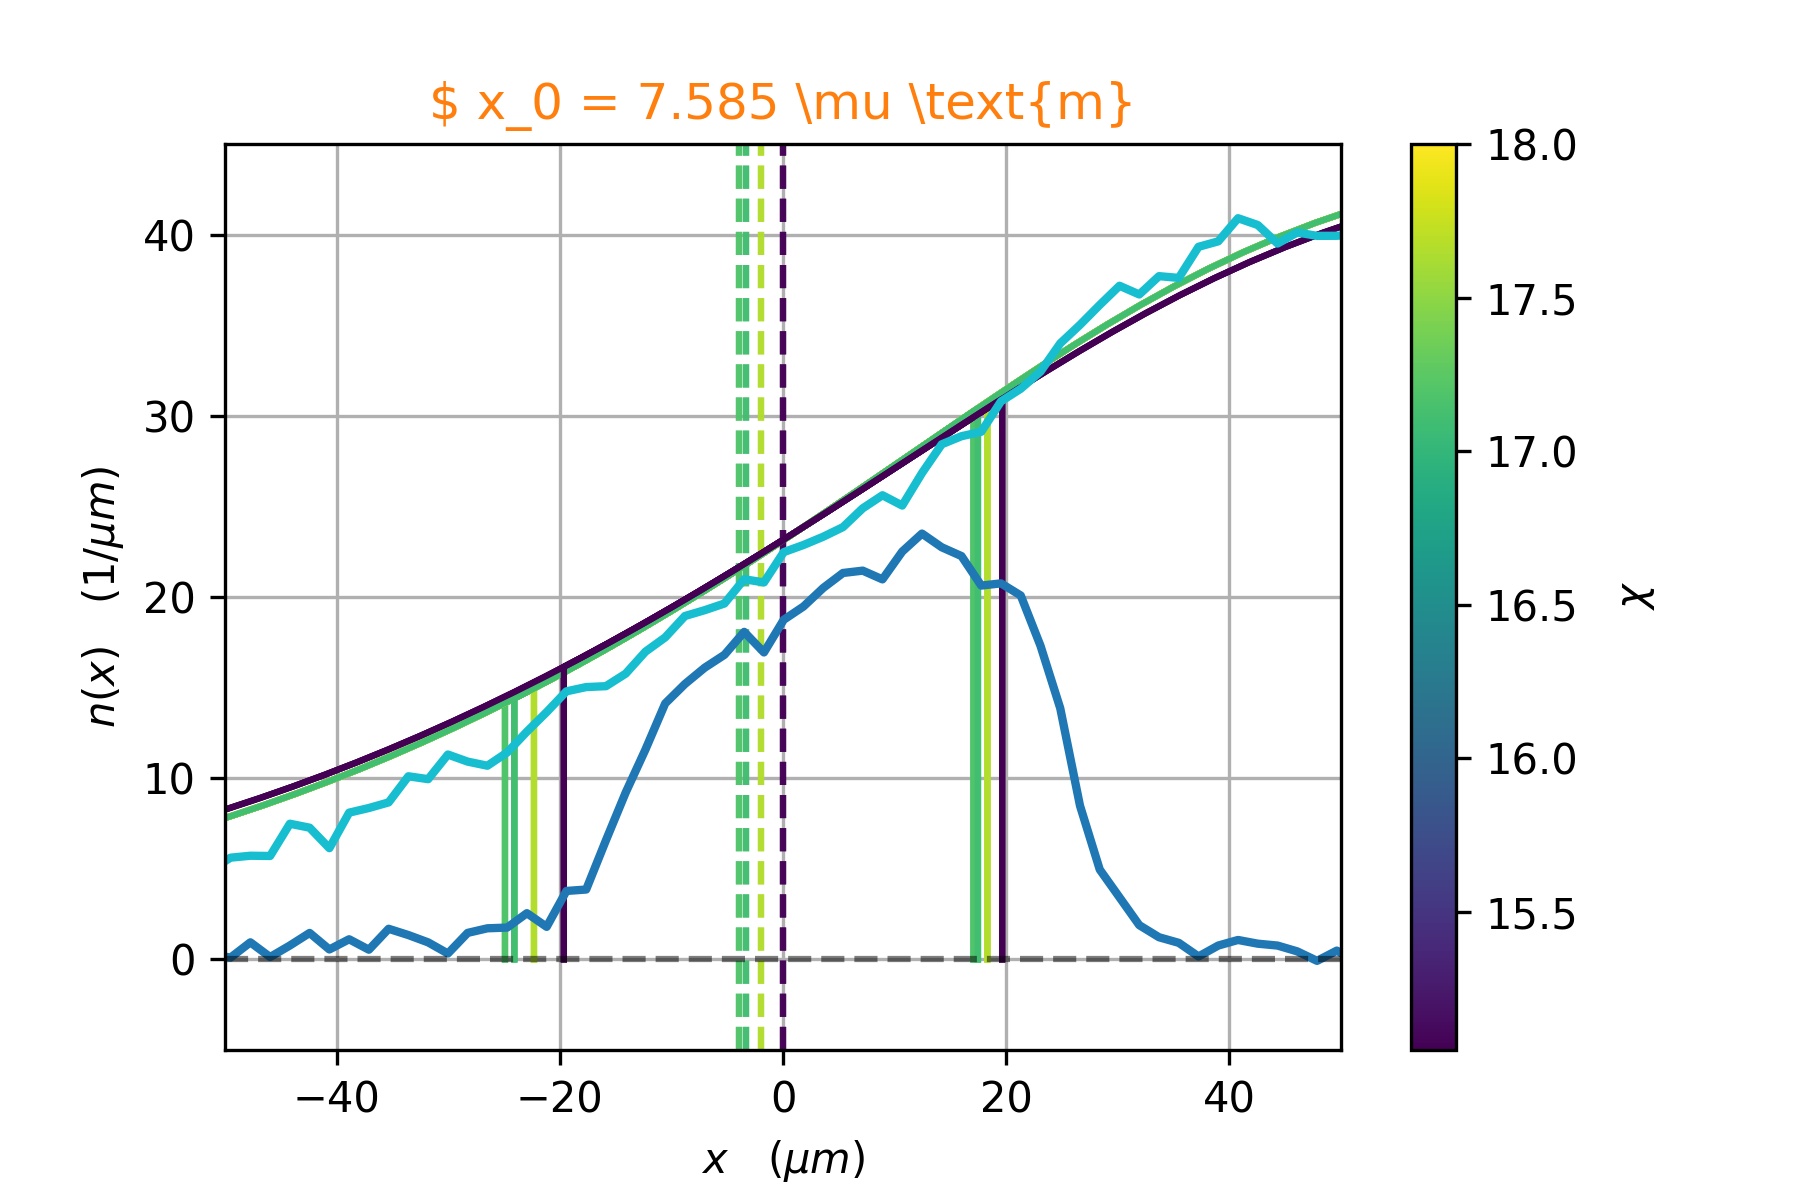
\includegraphics[width=\textwidth]{Figures/simul_deformation_T-x0_chi_09-02-2024}
        \caption{}
        \label{}
    \end{subfigure}
    \hfill
    \begin{subfigure}[b]{0.48\textwidth}
        \centering
        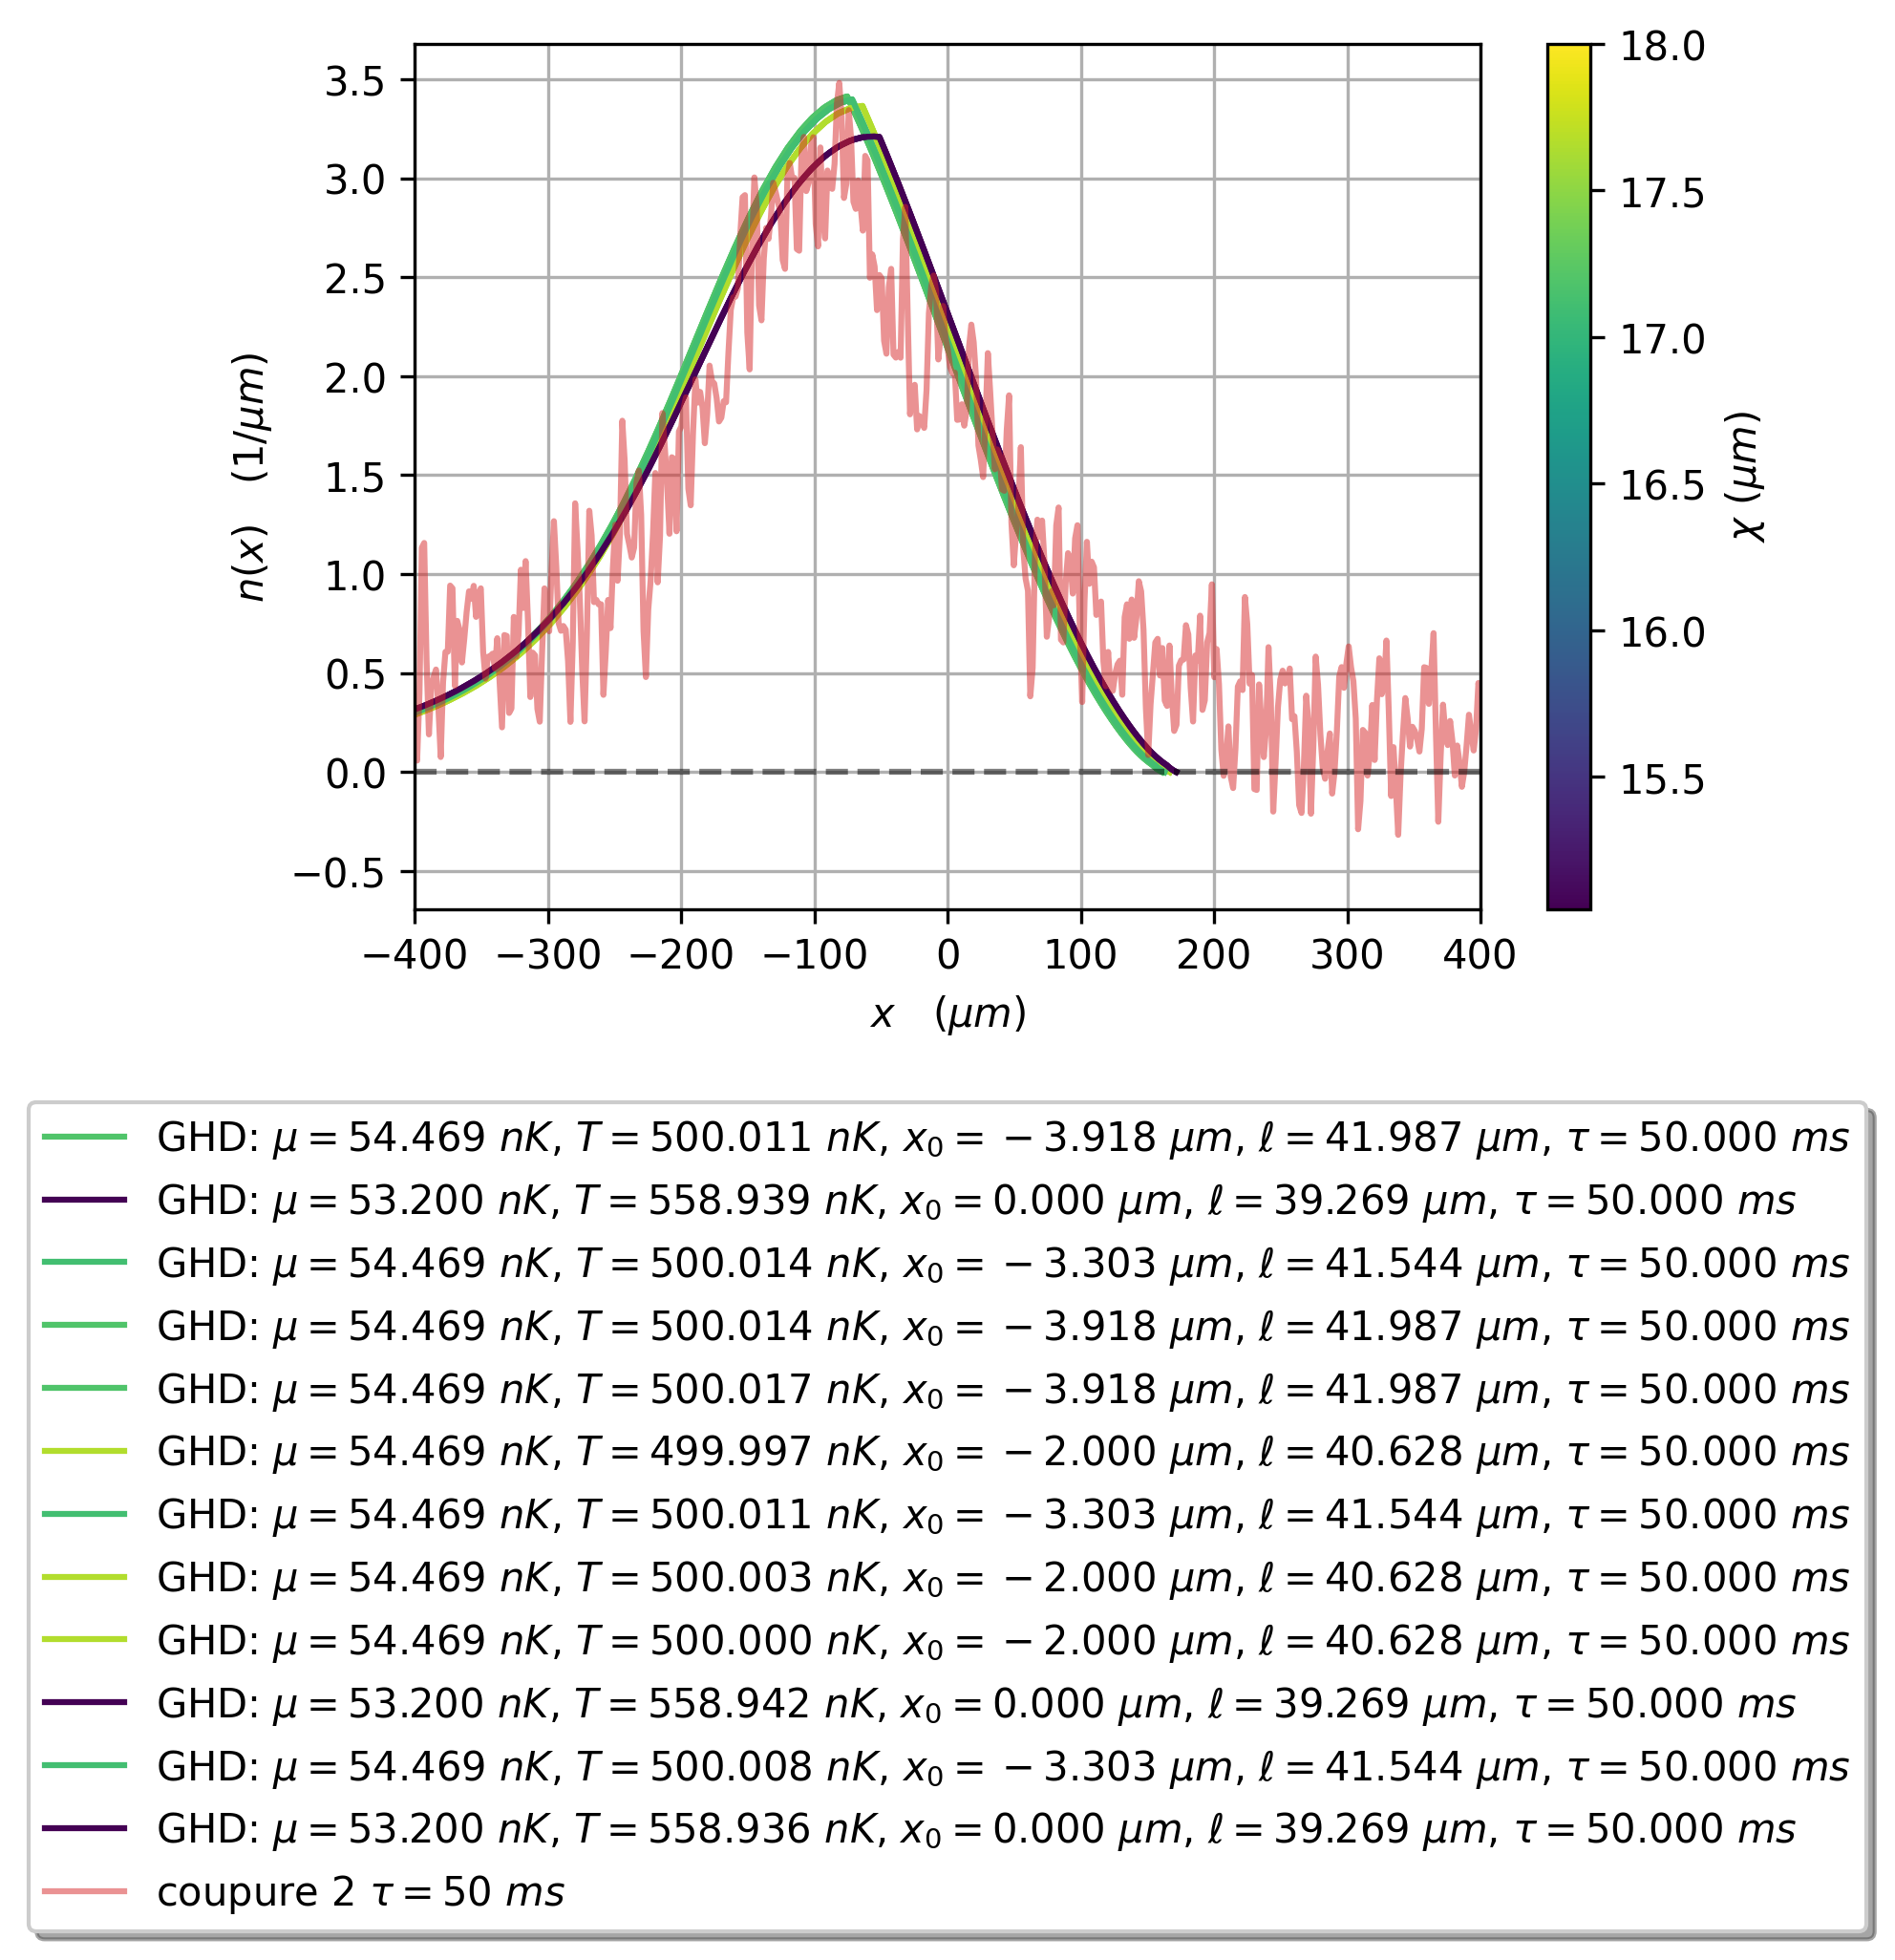
\includegraphics[width=\textwidth]{Figures/simul_expansion_T-x0_chi_09-02-2024}
        \caption{}
        \label{}
    \end{subfigure}


    \caption{Donnée du 09-02-24}
    \label{}
\end{figure}

	
	\begin{figure}[H]
	\centering
    
    \begin{subfigure}[b]{0.48\textwidth}
        \centering
        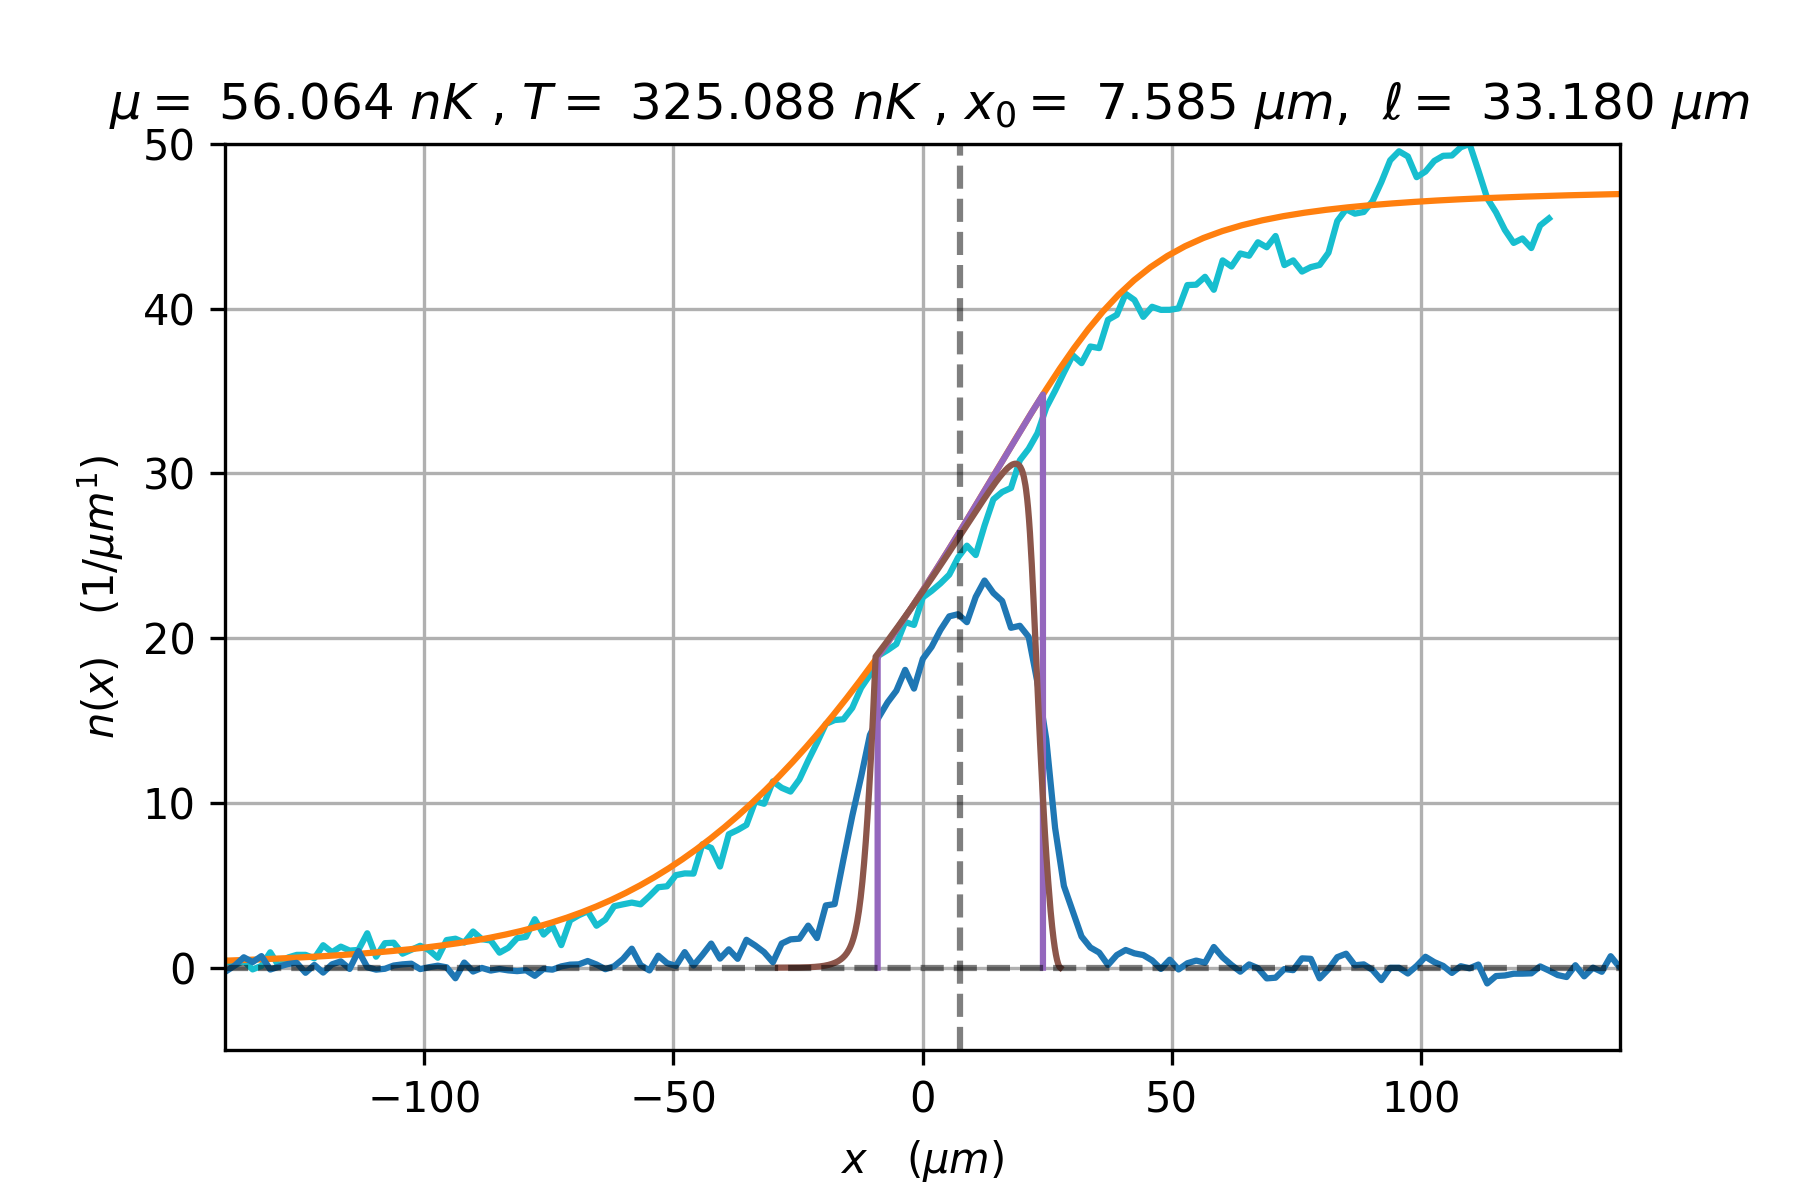
\includegraphics[width=\textwidth]{Figures/simul_deformation_1_09-02-2024}
        \caption{}
        \label{}
    \end{subfigure}
    \hfill
    \begin{subfigure}[b]{0.48\textwidth}
        \centering
        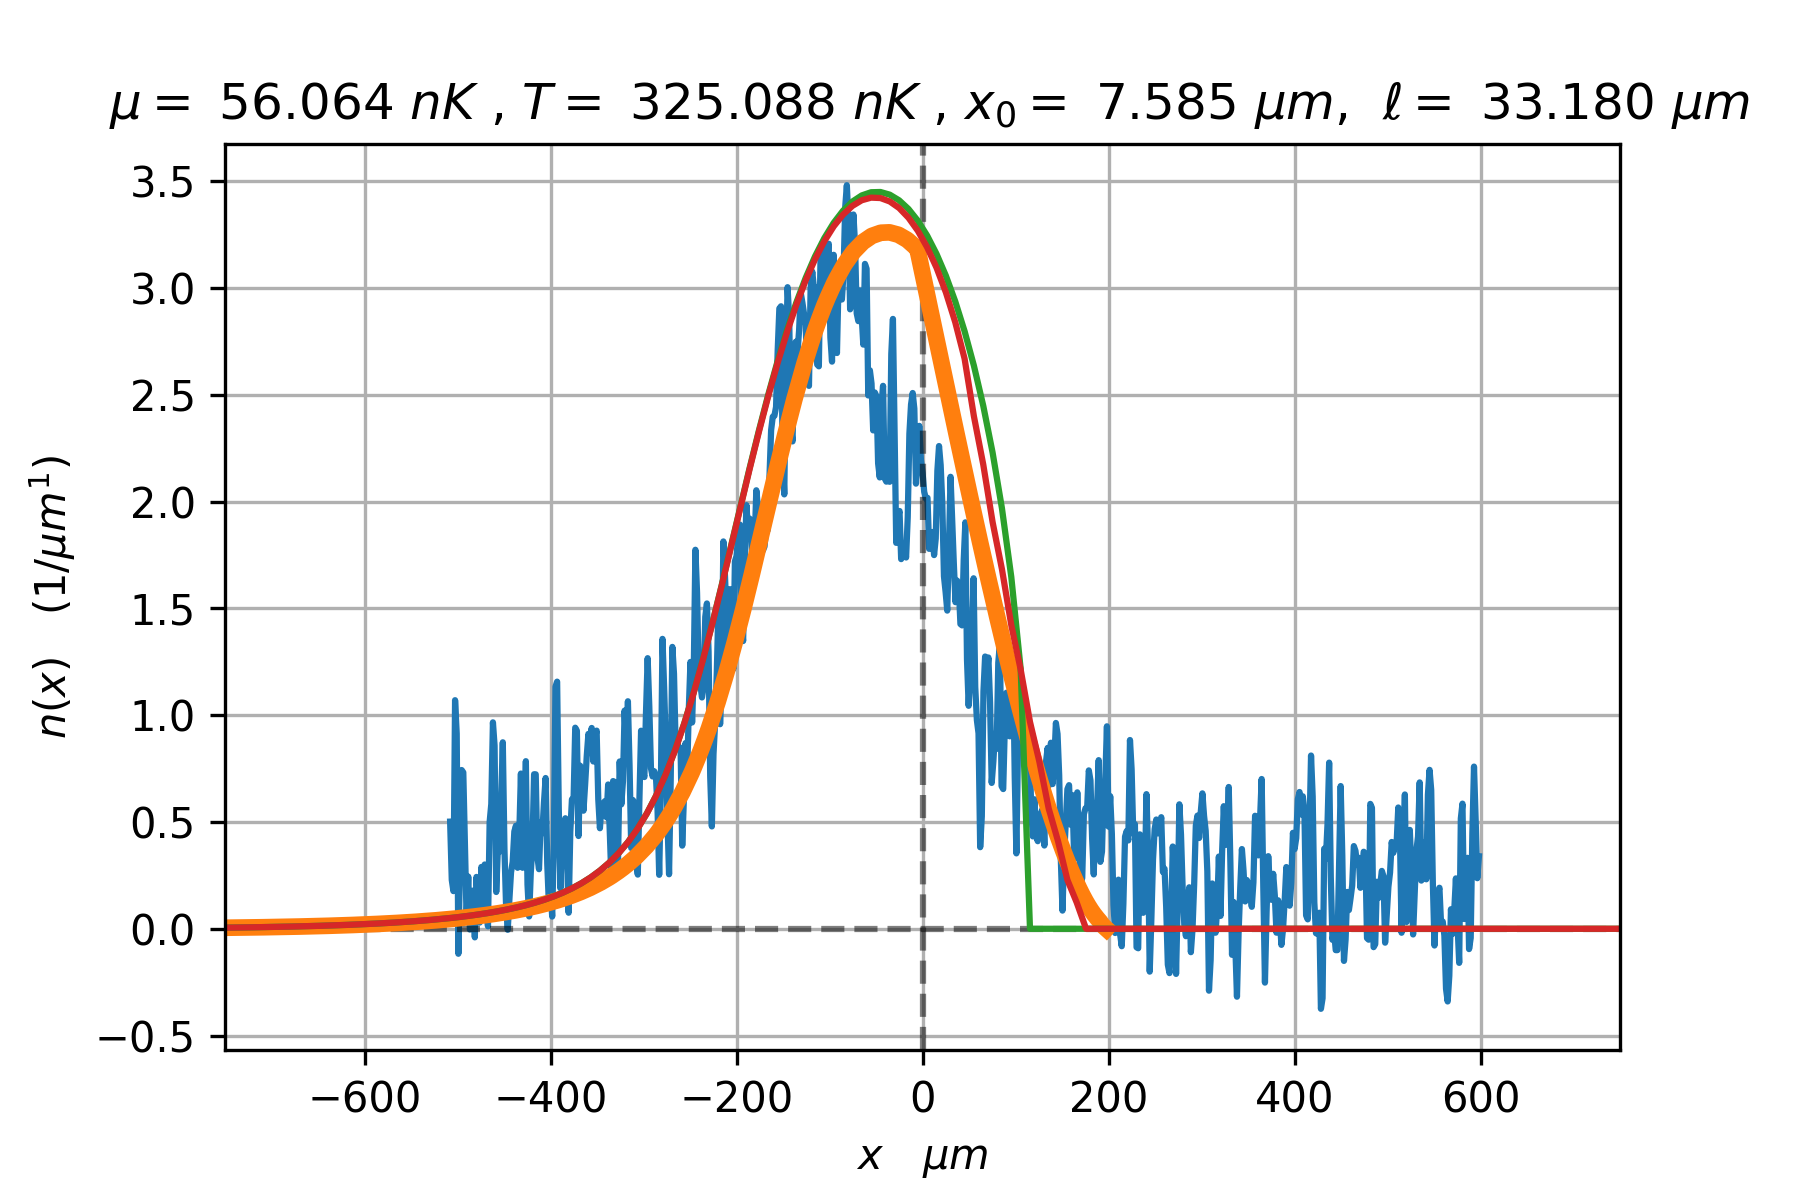
\includegraphics[width=\textwidth]{Figures/simul_expansion_1_09-02-2024}
        \caption{}
        \label{}
    \end{subfigure}
    \vspace{1em}
    \begin{subfigure}[b]{0.48\textwidth}
        \centering
        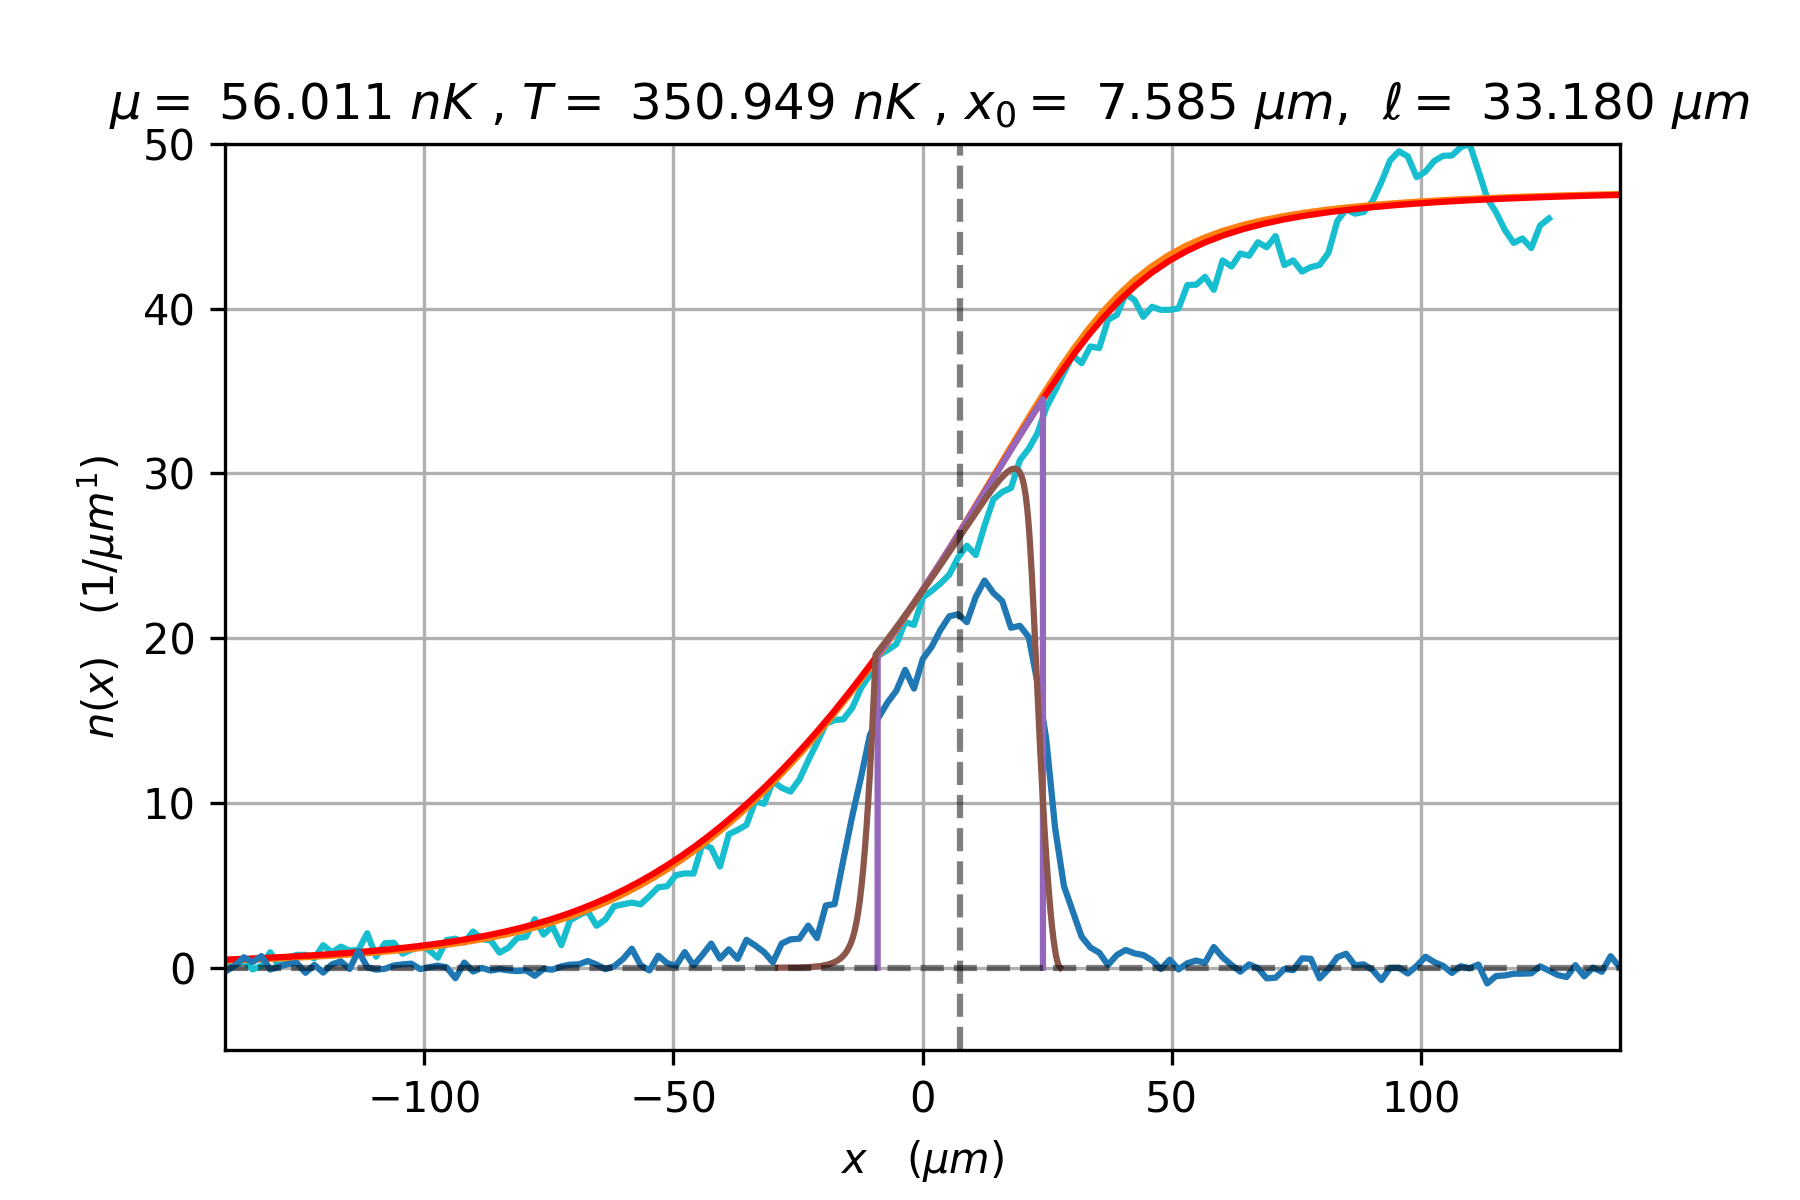
\includegraphics[width=\textwidth]{Figures/simul_deformation_2_09-02-2024}
        \caption{}
        \label{}
    \end{subfigure}
    \hfill
    \begin{subfigure}[b]{0.48\textwidth}
        \centering
        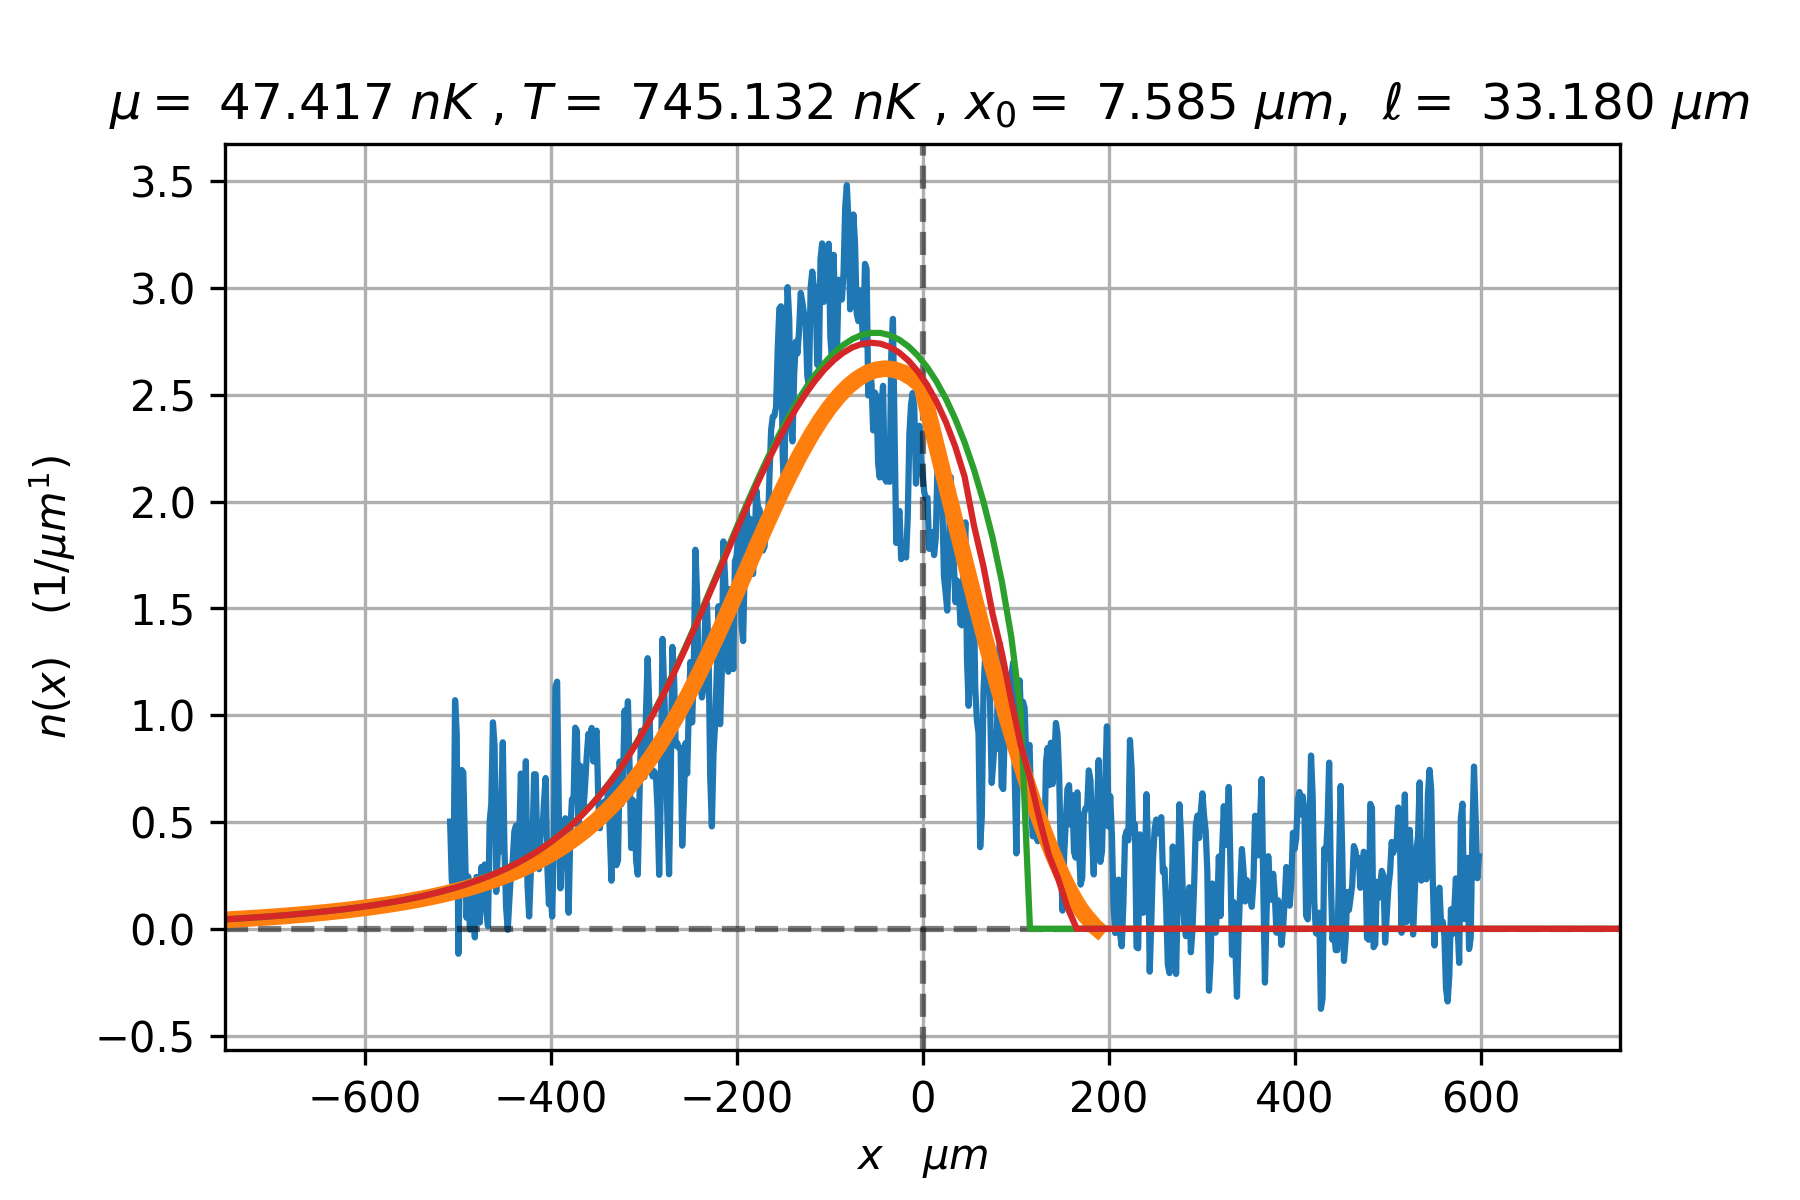
\includegraphics[width=\textwidth]{Figures/simul_expansion_2_09-02-2024}
        \caption{}
        \label{}
    \end{subfigure}
    \vspace{1em}
    \begin{subfigure}[b]{0.48\textwidth}
        \centering
        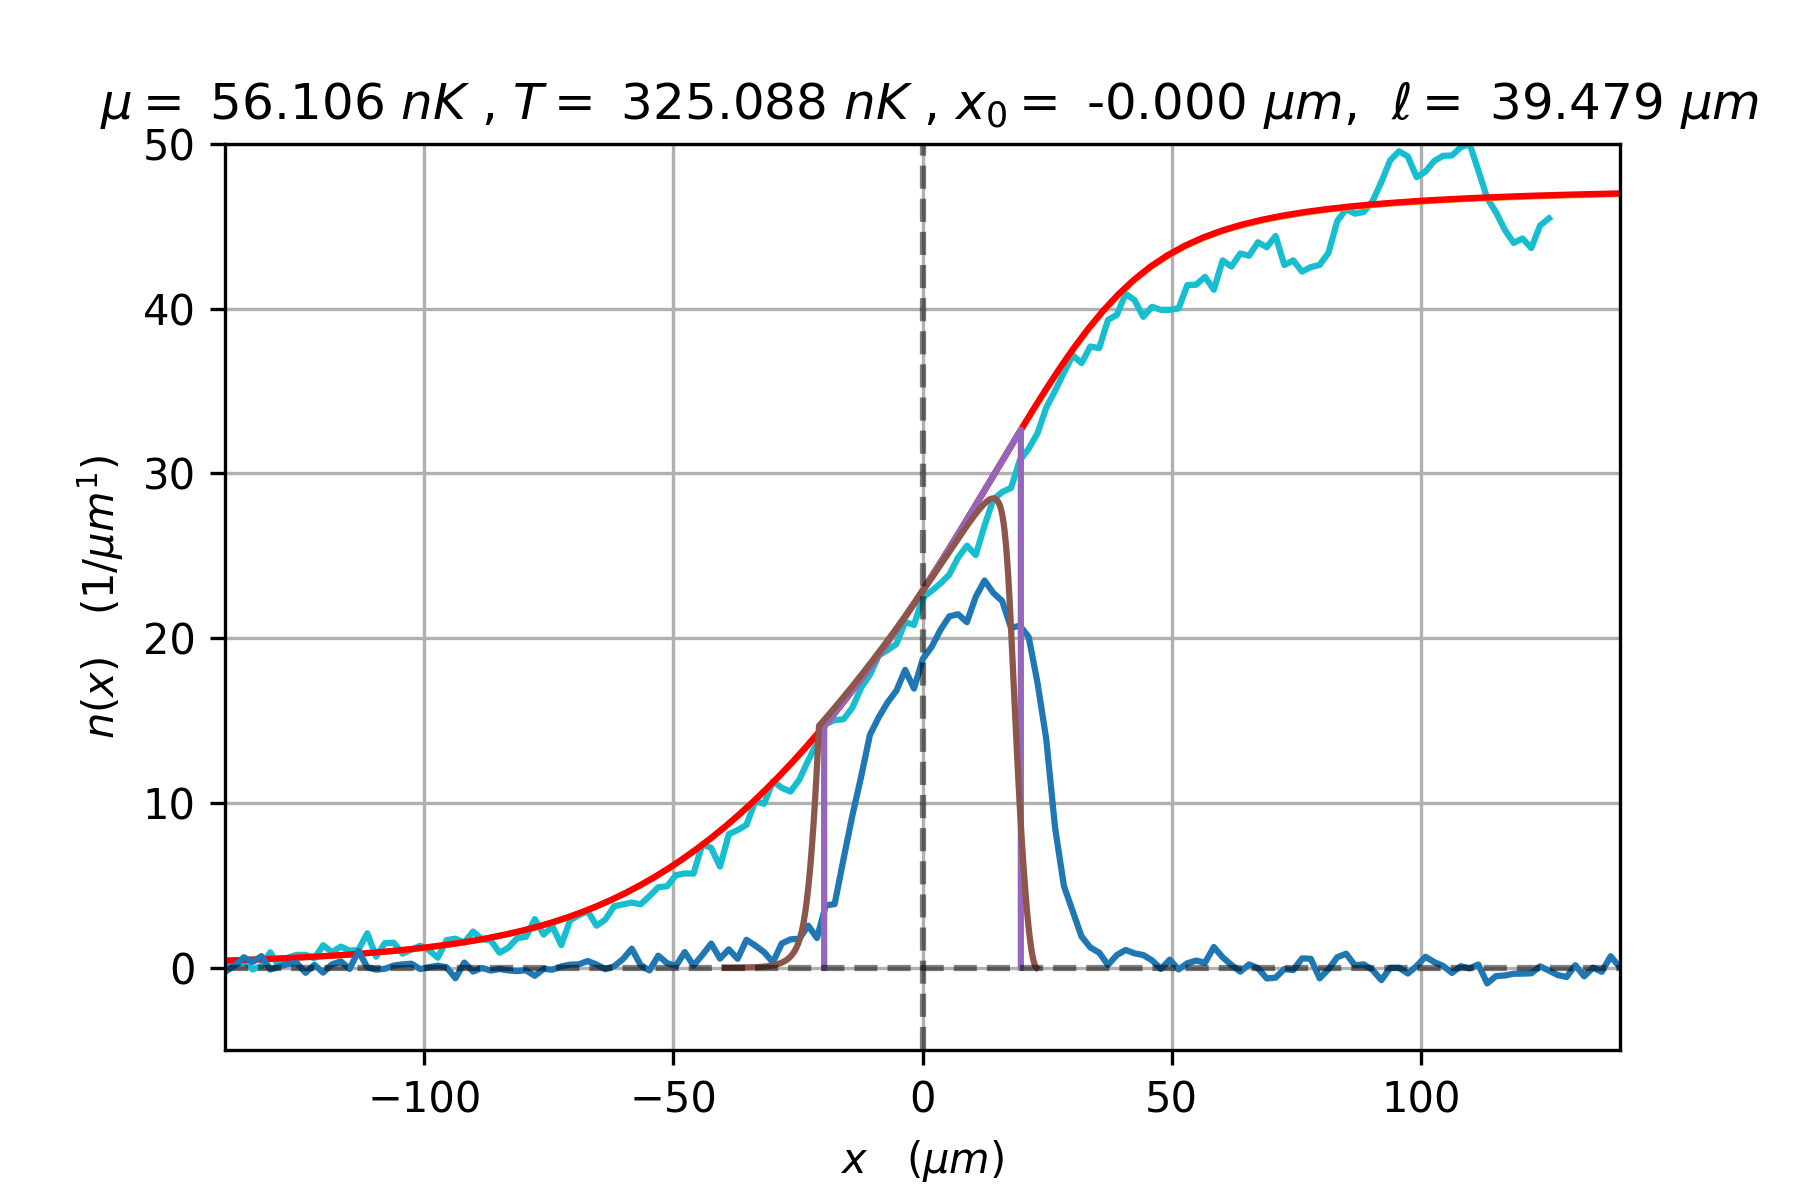
\includegraphics[width=\textwidth]{Figures/simul_deformation_3_09-02-2024}
        \caption{}
        \label{}
    \end{subfigure}
    \hfill
    \begin{subfigure}[b]{0.48\textwidth}
        \centering
        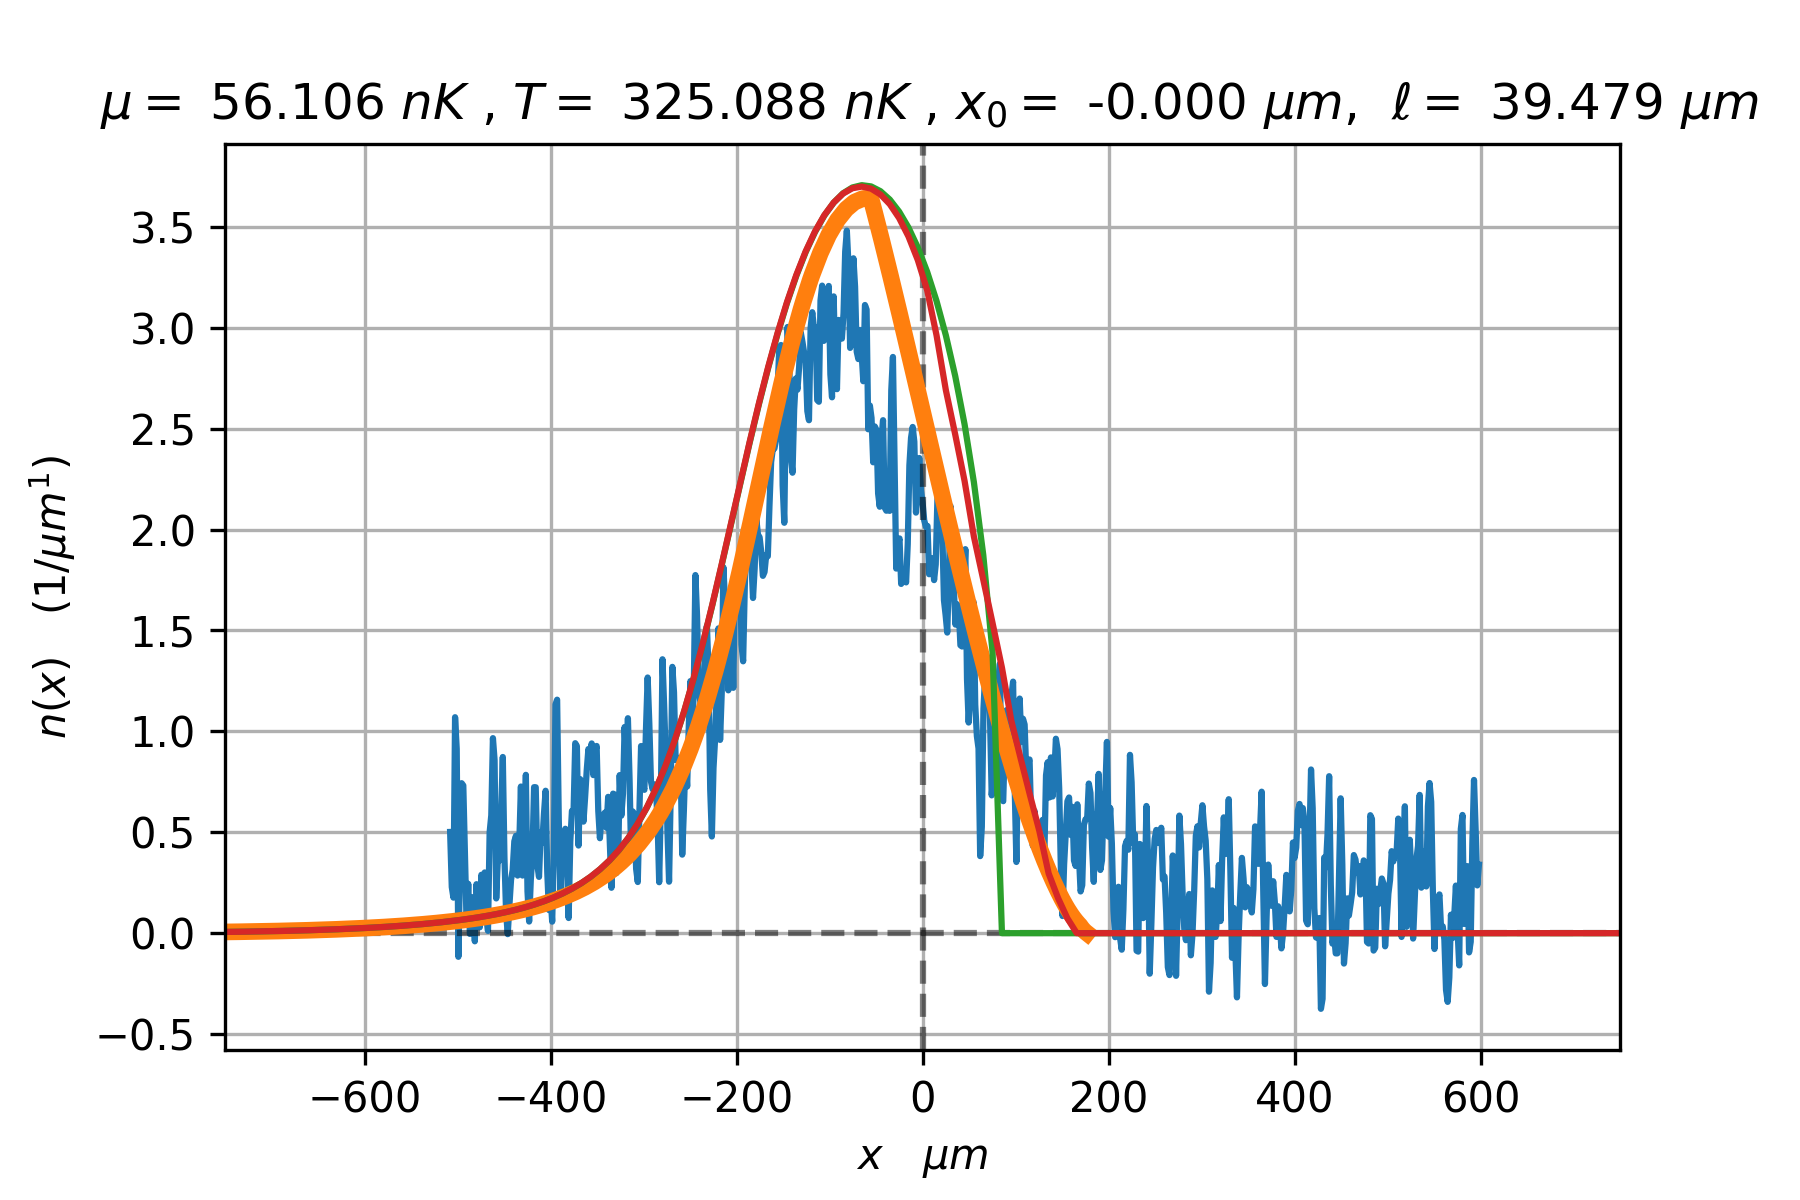
\includegraphics[width=\textwidth]{Figures/simul_expansion_3_09-02-2024}
        \caption{}
        \label{}
    \end{subfigure}
    \vspace{1em}
    \begin{subfigure}[b]{0.48\textwidth}
        \centering
        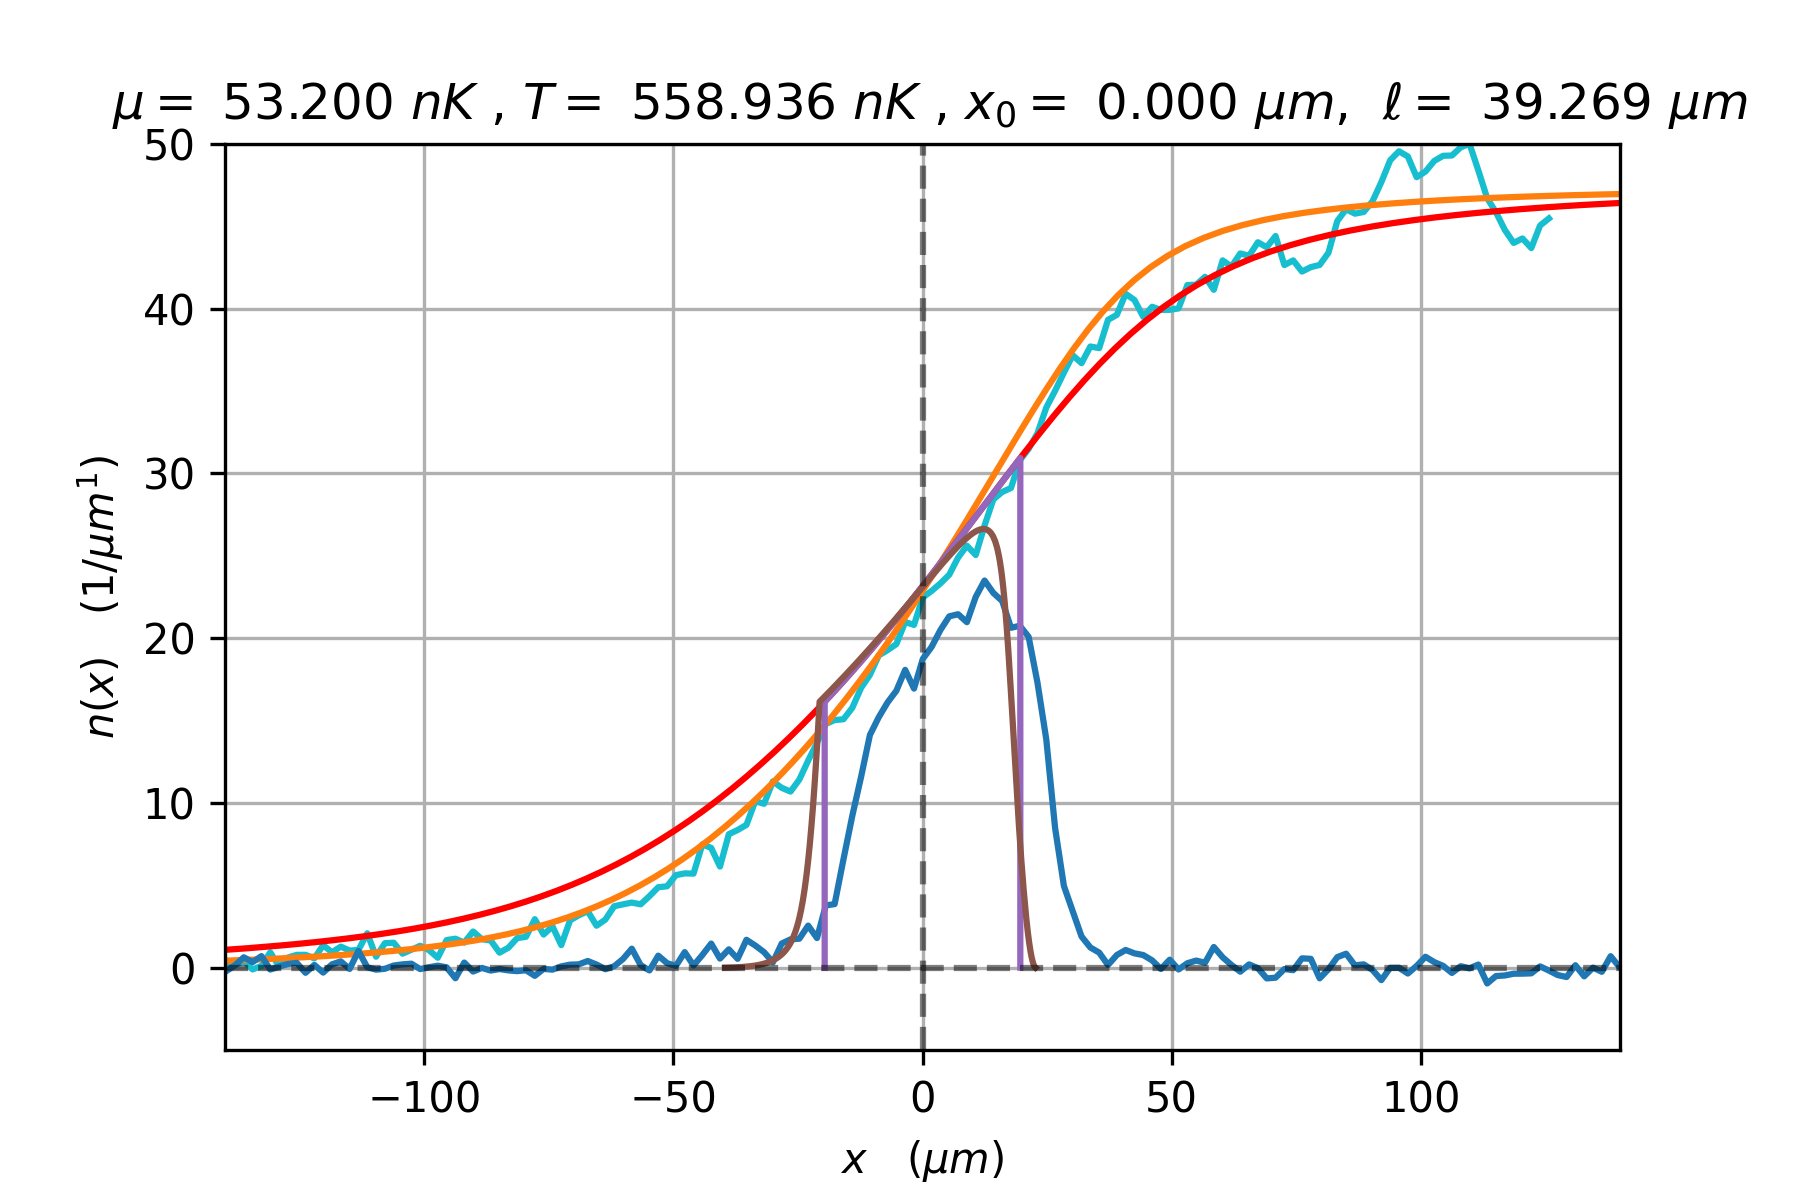
\includegraphics[width=\textwidth]{Figures/simul_deformation_4_09-02-2024}
        \caption{}
        \label{}
    \end{subfigure}
    \hfill
    \begin{subfigure}[b]{0.48\textwidth}
        \centering
        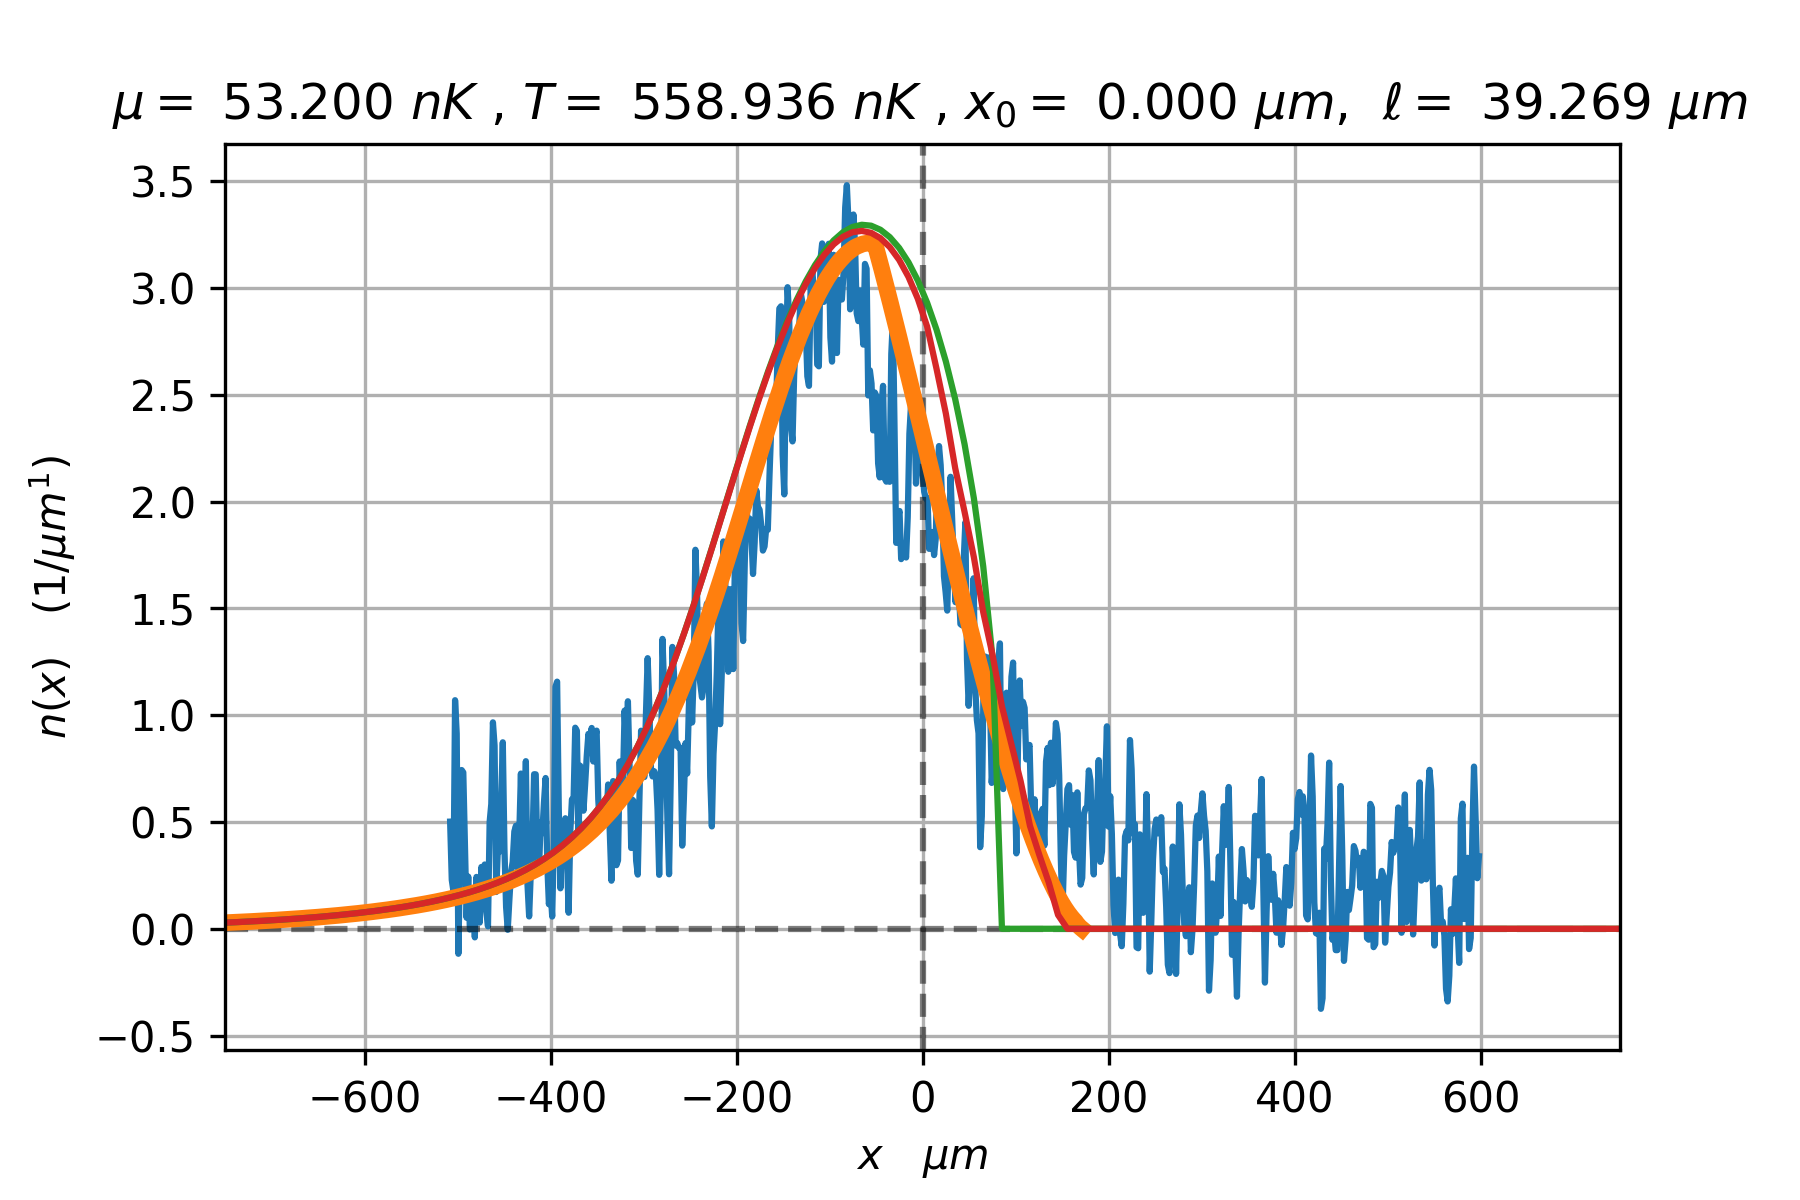
\includegraphics[width=\textwidth]{Figures/simul_expansion_4_09-02-2024}
        \caption{}
        \label{}
    \end{subfigure}

    \caption{Donnée du 09-02-24}
    \label{}
\end{figure}


	
	\begin{figure}[H]
	\centering

    
    \begin{subfigure}[b]{0.48\textwidth}
        \centering
        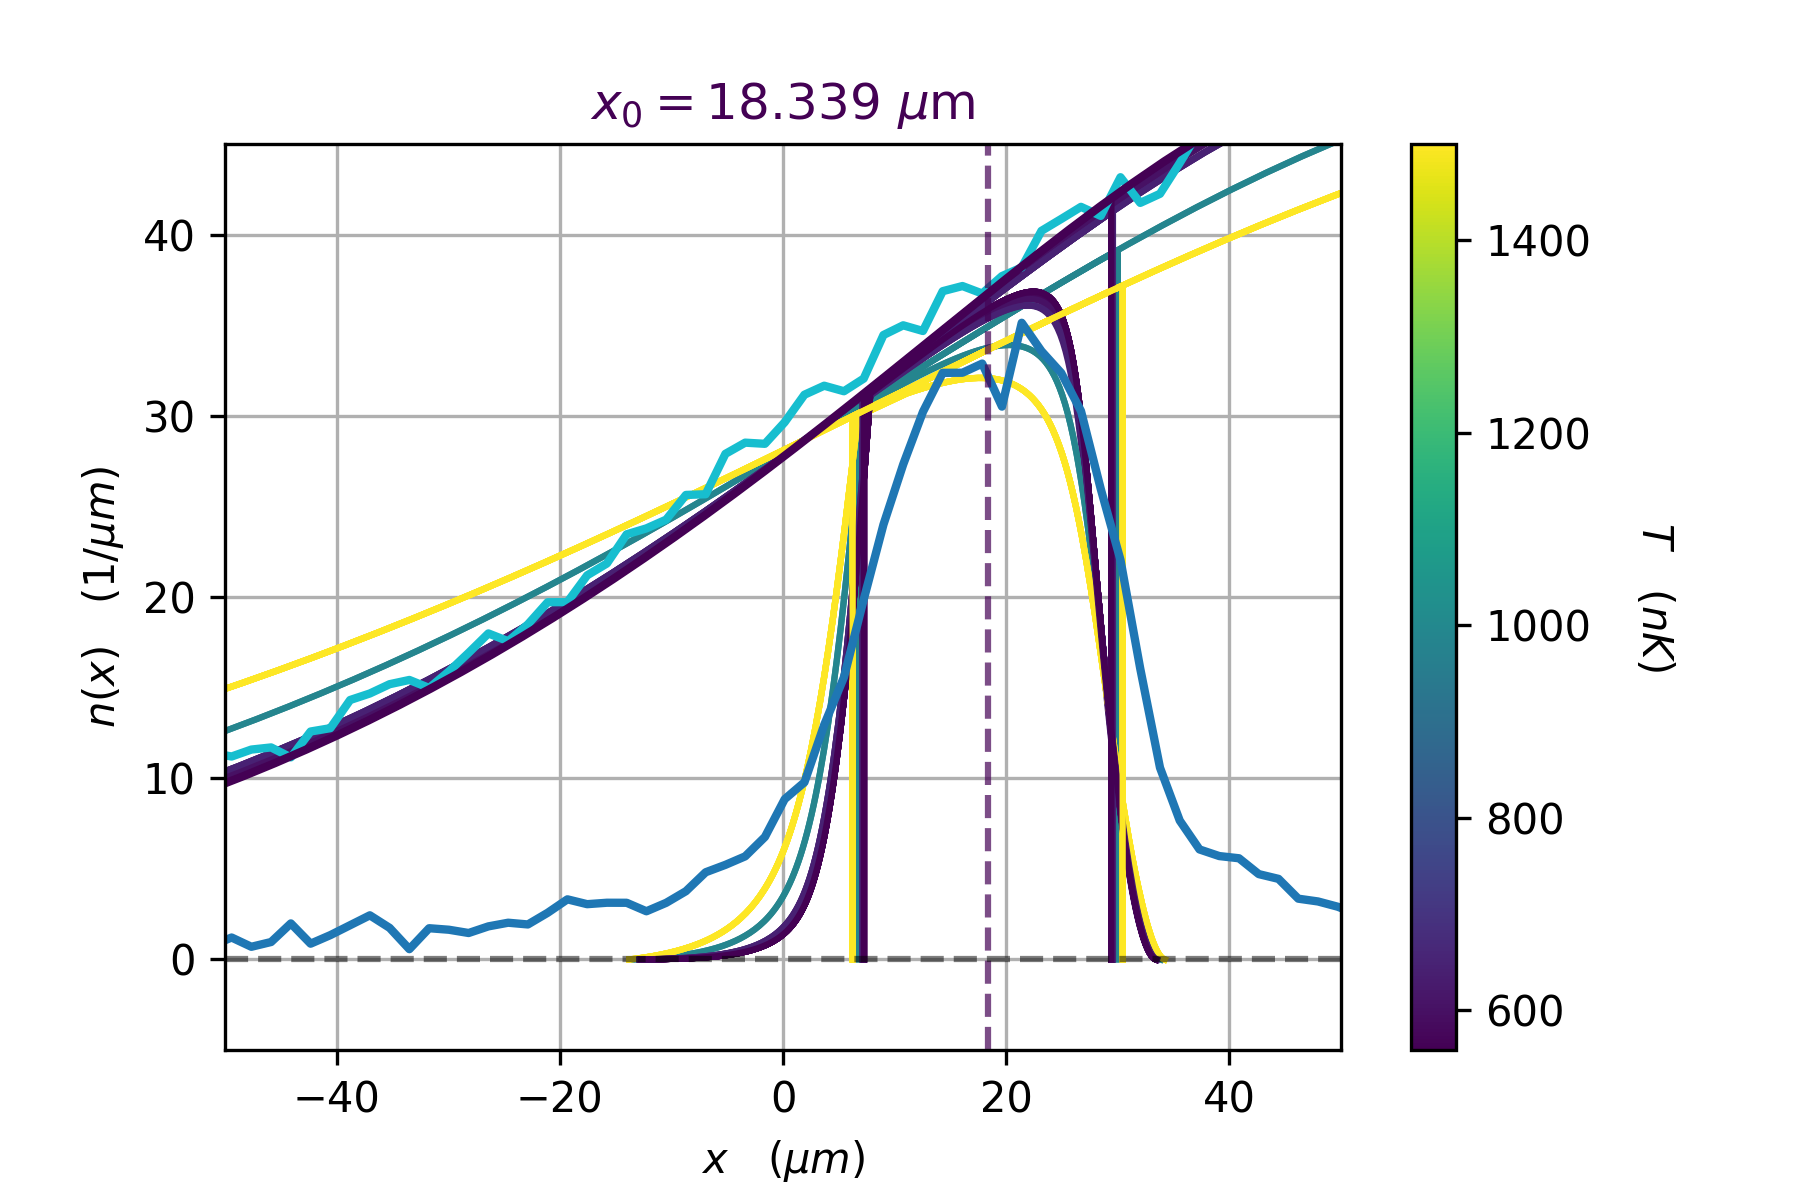
\includegraphics[width=\textwidth]{Figures/simul_deformation_T_24-04-2024}
        \caption{}
        \label{}
    \end{subfigure}
    \hfill
    \begin{subfigure}[b]{0.48\textwidth}
        \centering
        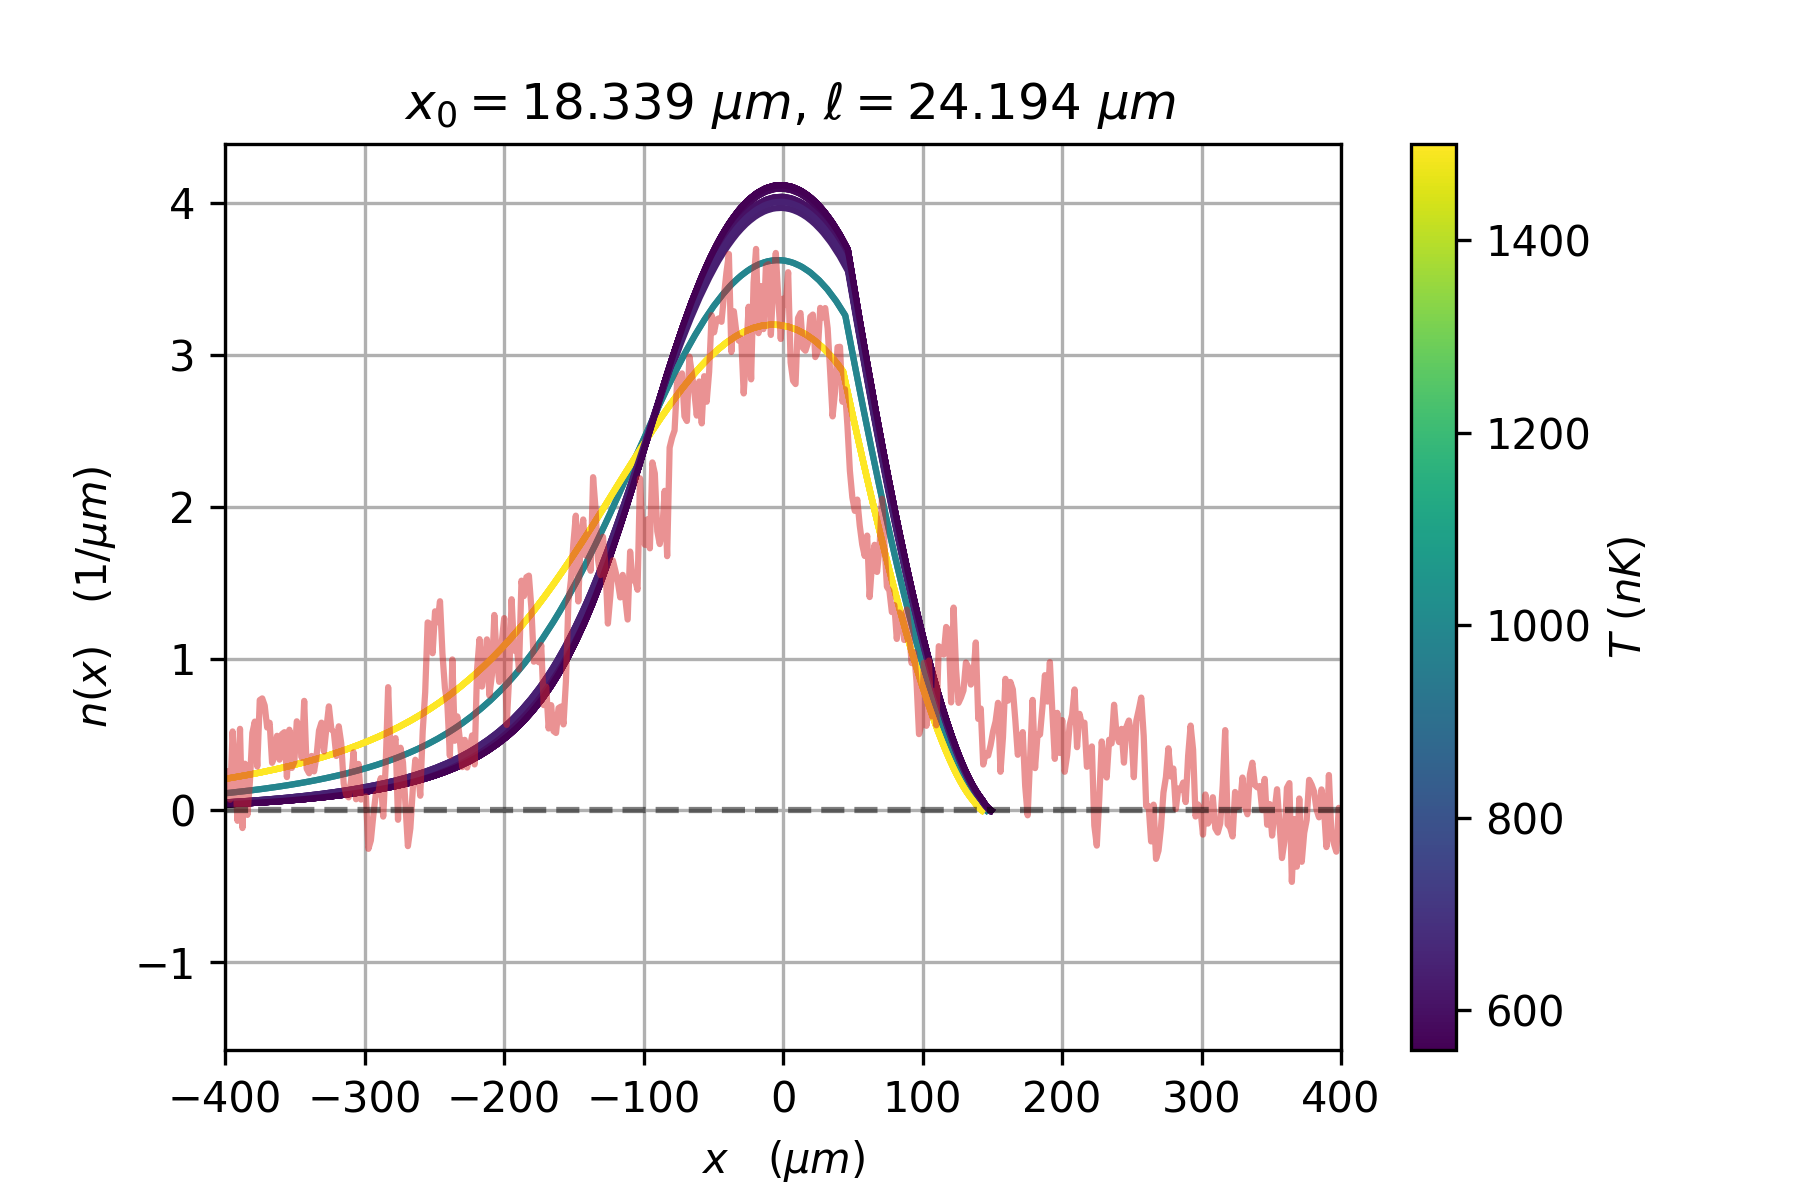
\includegraphics[width=\textwidth]{Figures/simul_expansion_T_24-04-2024}
        \caption{}
        \label{}
    \end{subfigure}
    \vspace{1em}
    \begin{subfigure}[b]{0.48\textwidth}
        \centering
        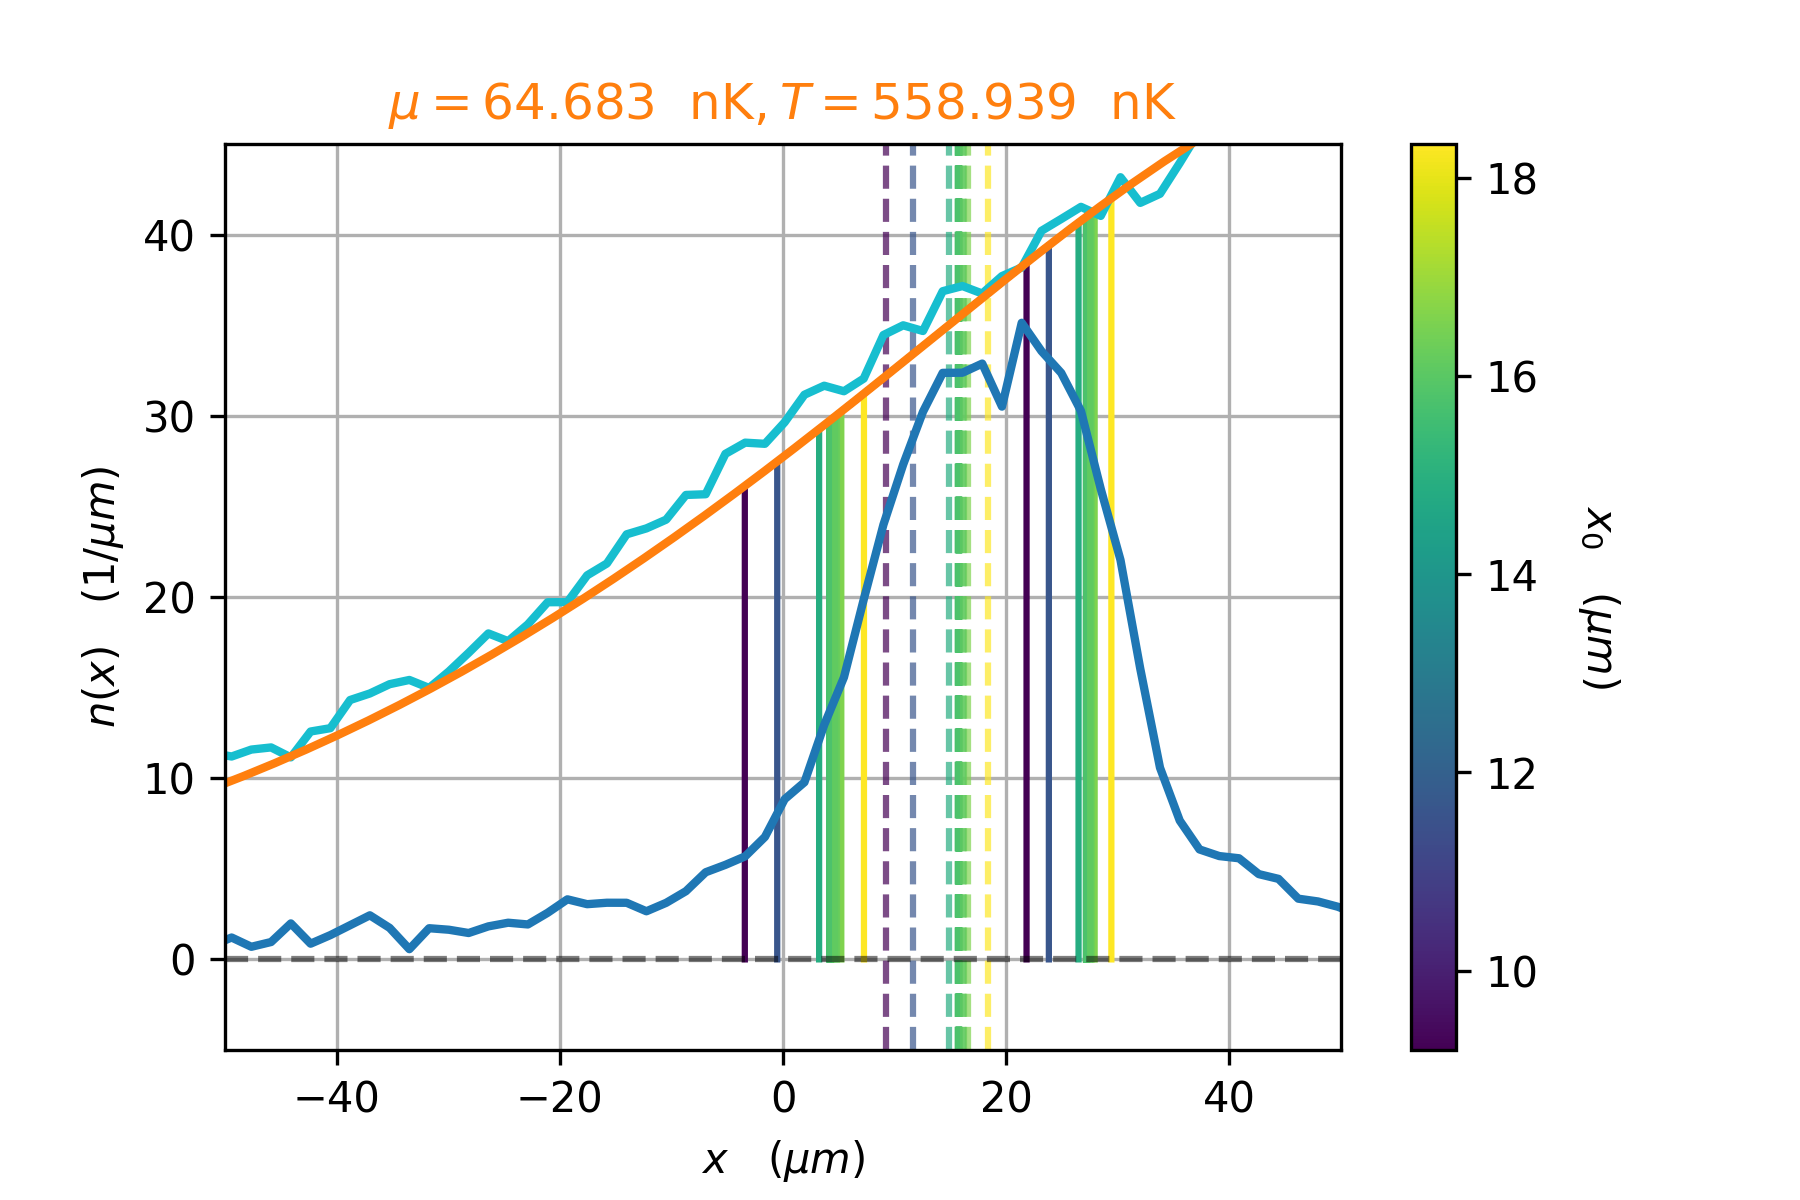
\includegraphics[width=\textwidth]{Figures/simul_deformation_x0_24-04-2024}
        \caption{}
        \label{}
    \end{subfigure}
    \hfill
    \begin{subfigure}[b]{0.48\textwidth}
        \centering
        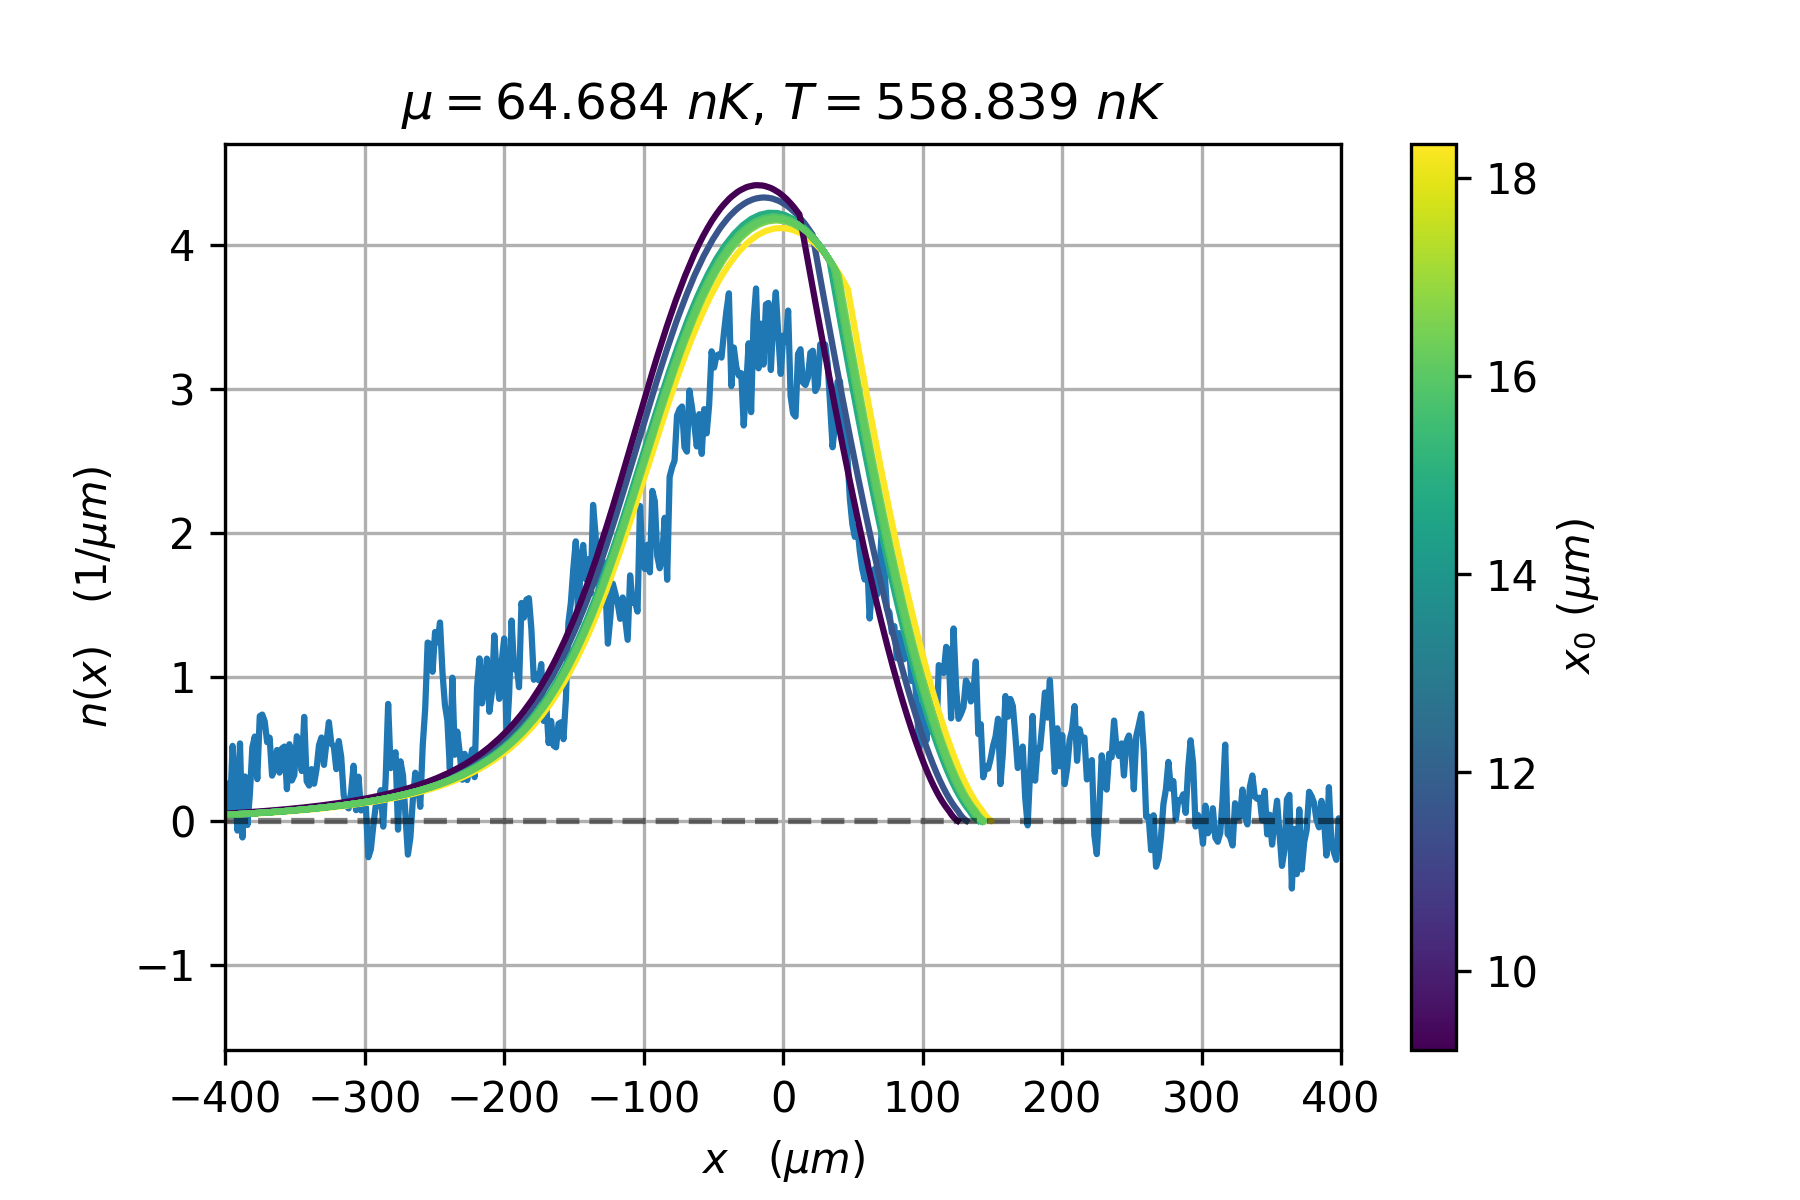
\includegraphics[width=\textwidth]{Figures/simul_expansion_x0_24-04-2024}
        \caption{}
        \label{}
    \end{subfigure}
    \vspace{1em}
    \begin{subfigure}[b]{0.48\textwidth}
        \centering
        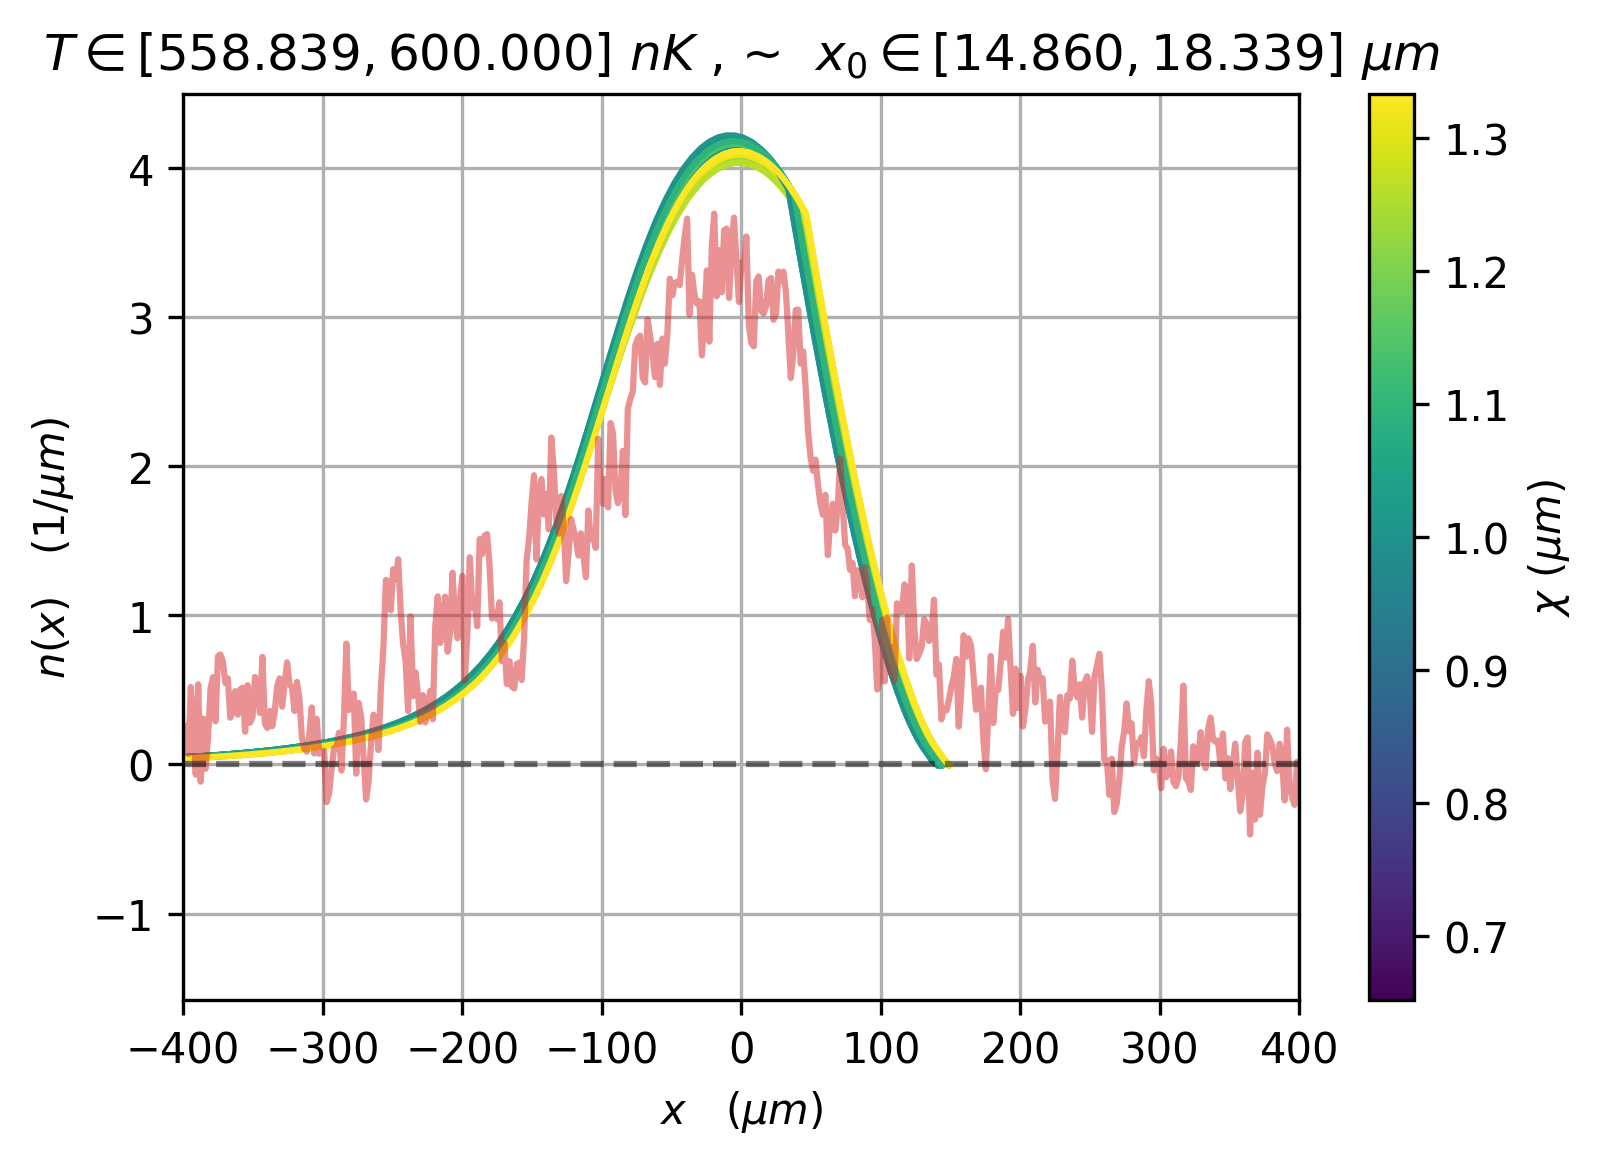
\includegraphics[width=\textwidth]{Figures/simul_expansion_T-x0-1_24-04-2024}
        \caption{}
        \label{}
    \end{subfigure}
    \hfill
	\begin{subfigure}[b]{0.48\textwidth}
        \centering
        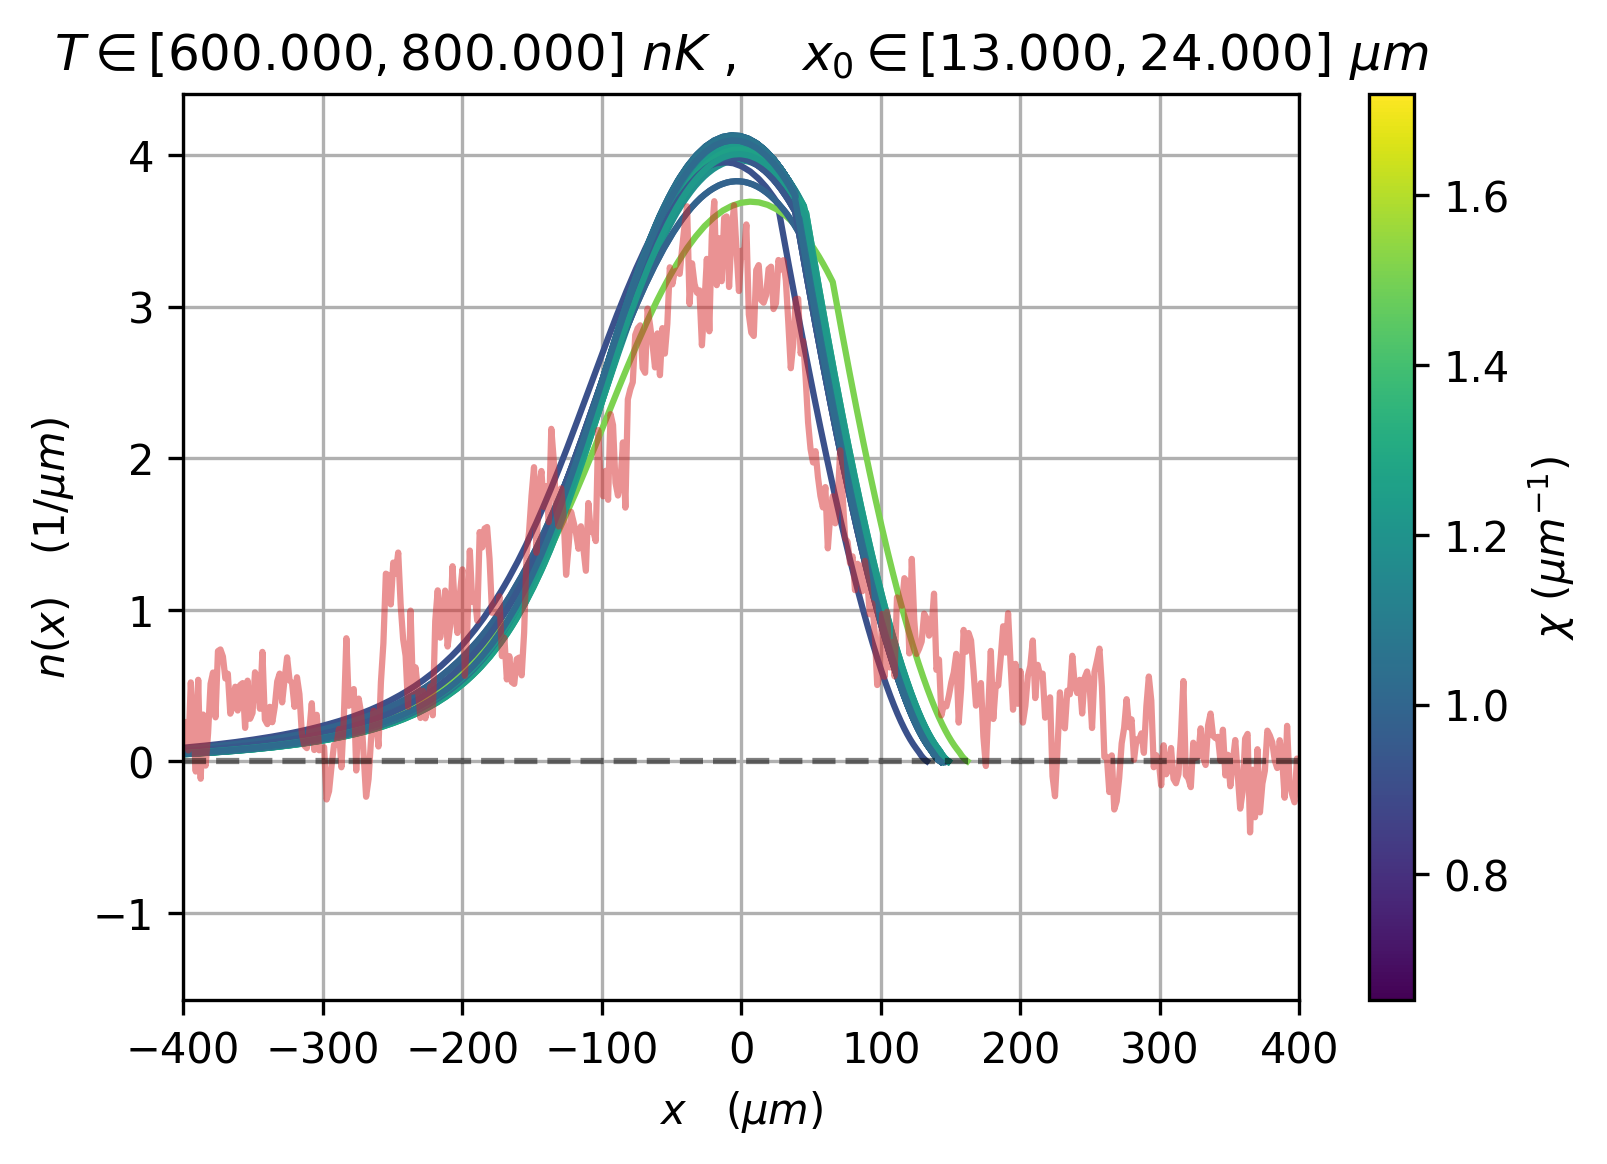
\includegraphics[width=\textwidth]{Figures/simul_expansion_T-x0-2_24-04-2024}
        \caption{}
        \label{}
    \end{subfigure}
    \vspace{1em}
    \begin{subfigure}[b]{0.48\textwidth}
        \centering
        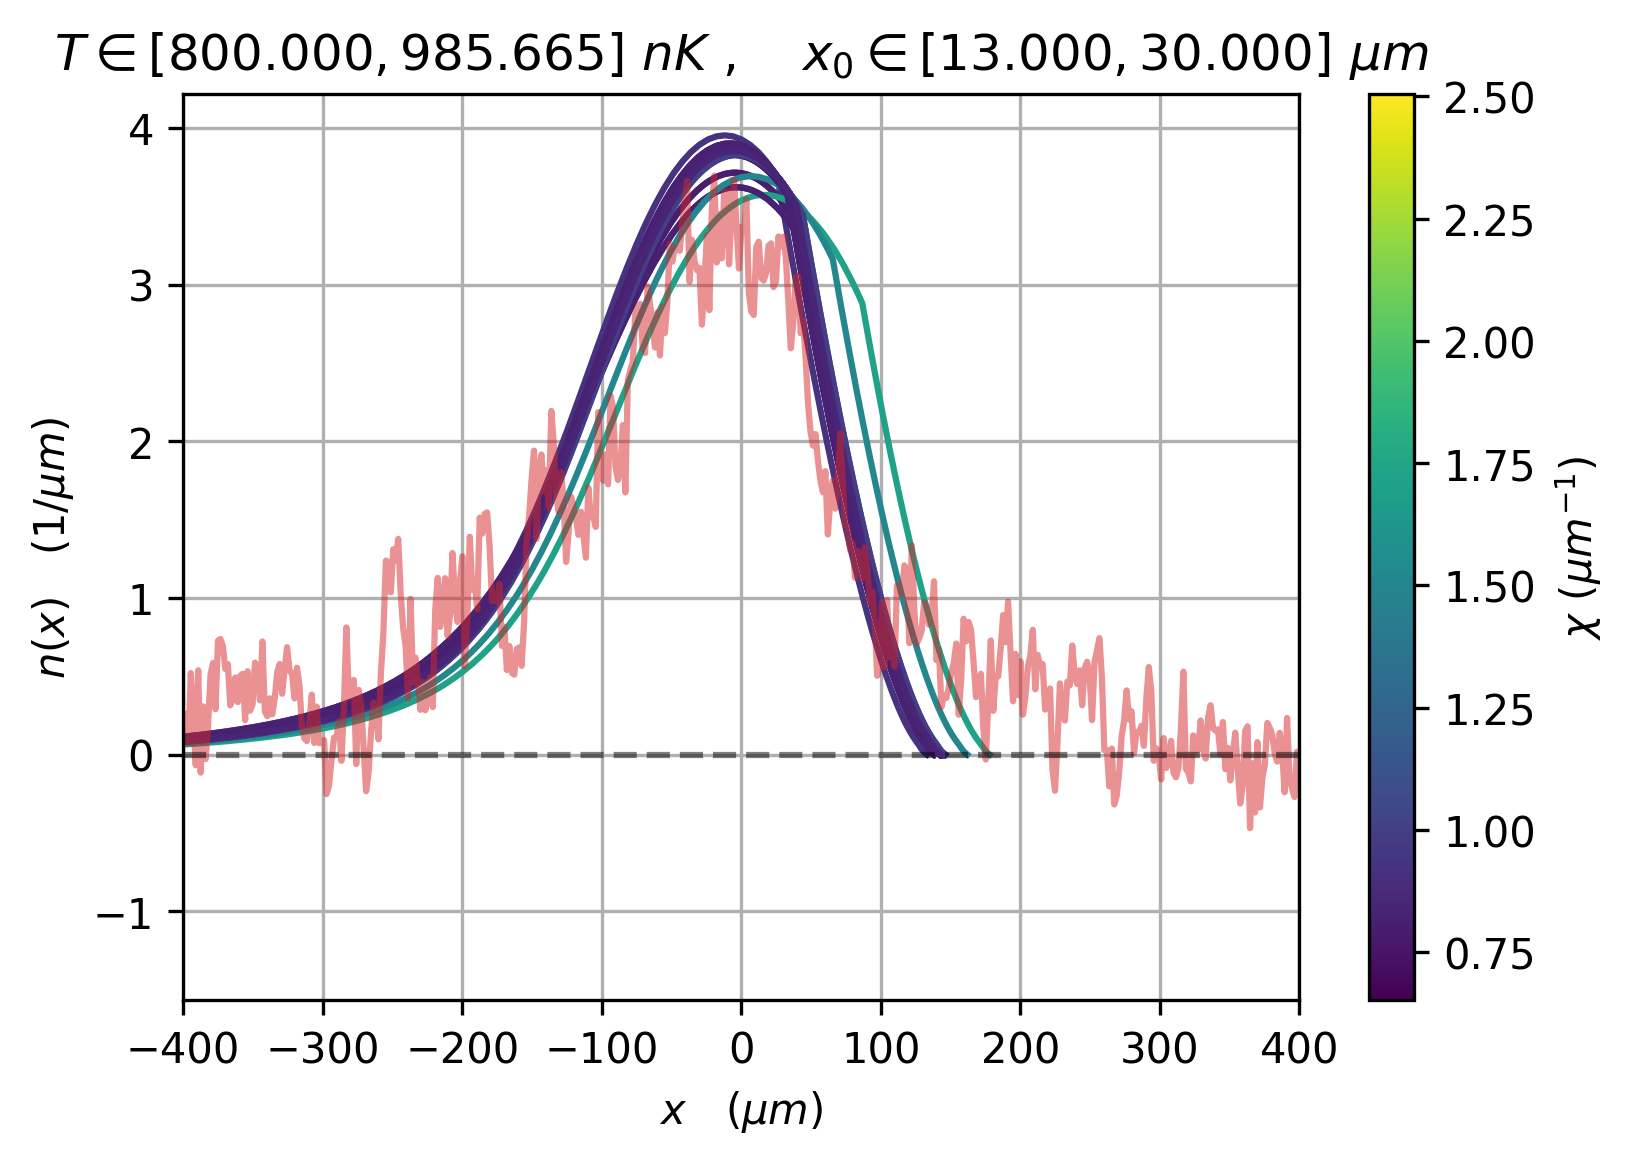
\includegraphics[width=\textwidth]{Figures/simul_expansion_T-x0-3_24-04-2024}
        \caption{}
        \label{}
    \end{subfigure}
    \hfill
	\begin{subfigure}[b]{0.48\textwidth}
        \centering
        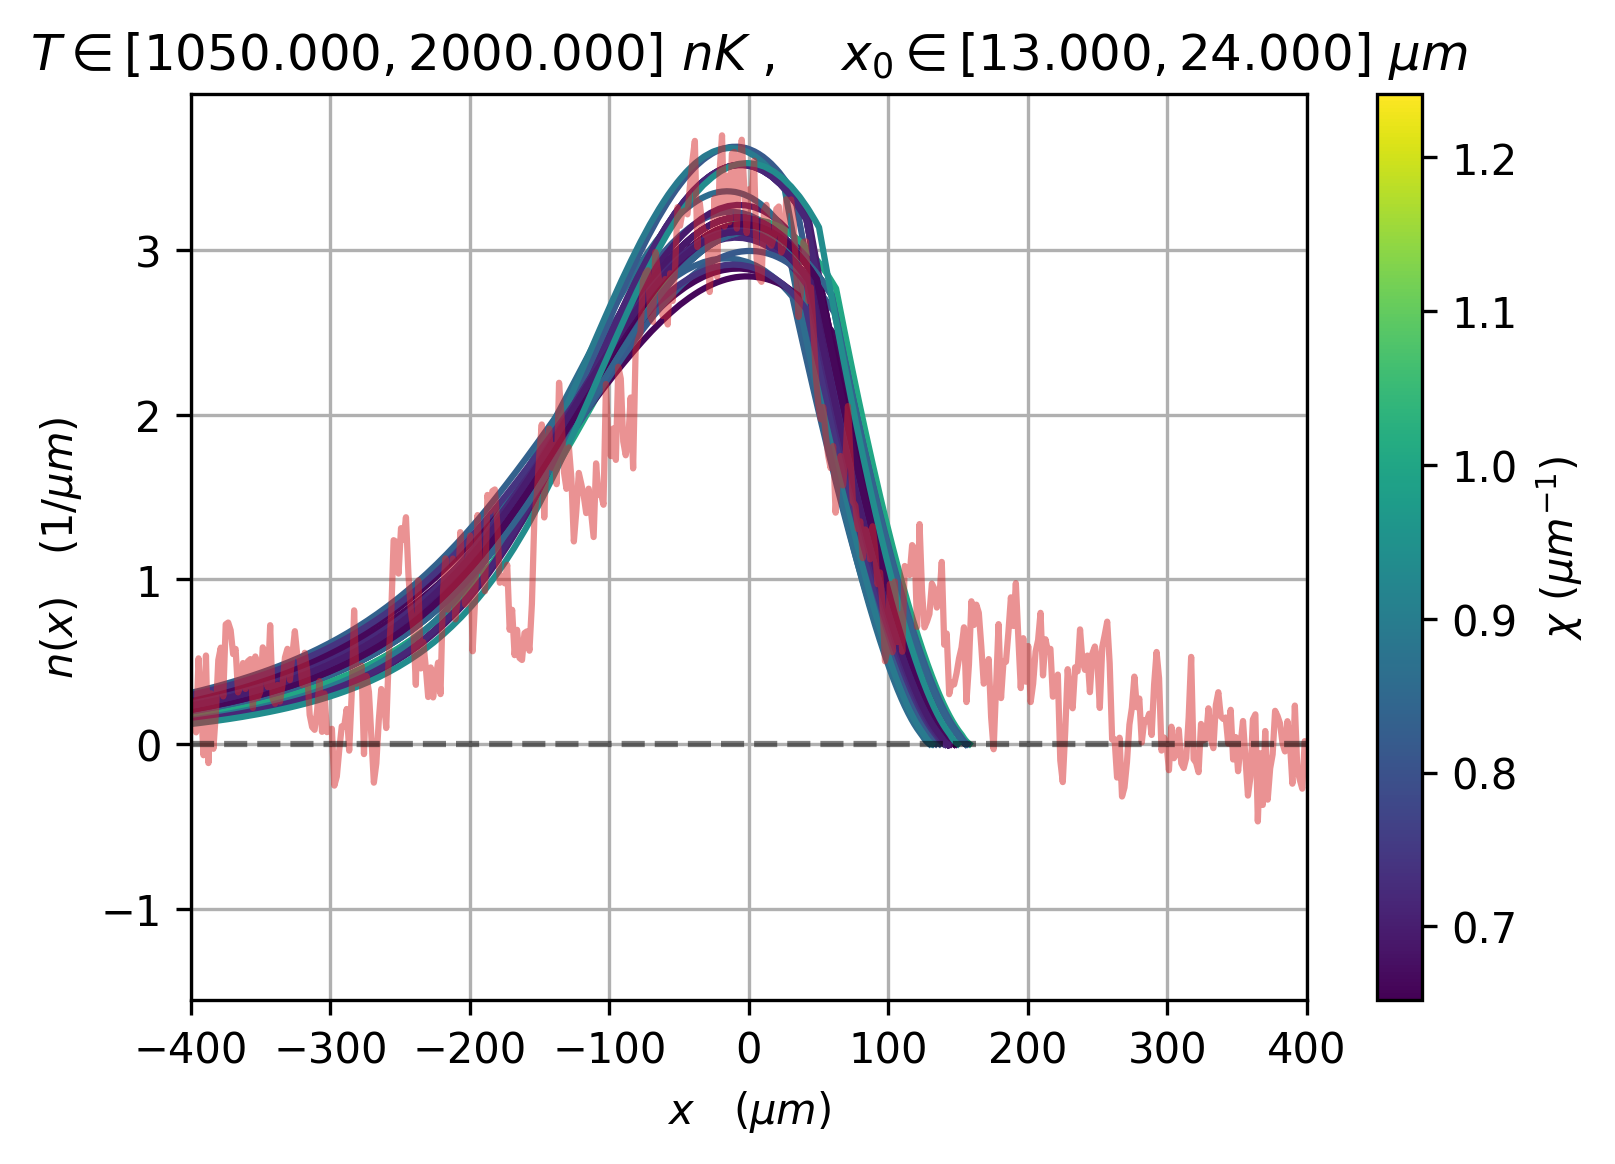
\includegraphics[width=\textwidth]{Figures/simul_expansion_T-x0-4_24-04-2024}
        \caption{}
        \label{}
    \end{subfigure}

    \caption{Donnée du 24-04-2024}
    \label{}
\end{figure}

\begin{figure}[H]
	\centering

 
    \vspace{1em}
    \begin{subfigure}[b]{1\textwidth}
        \centering
        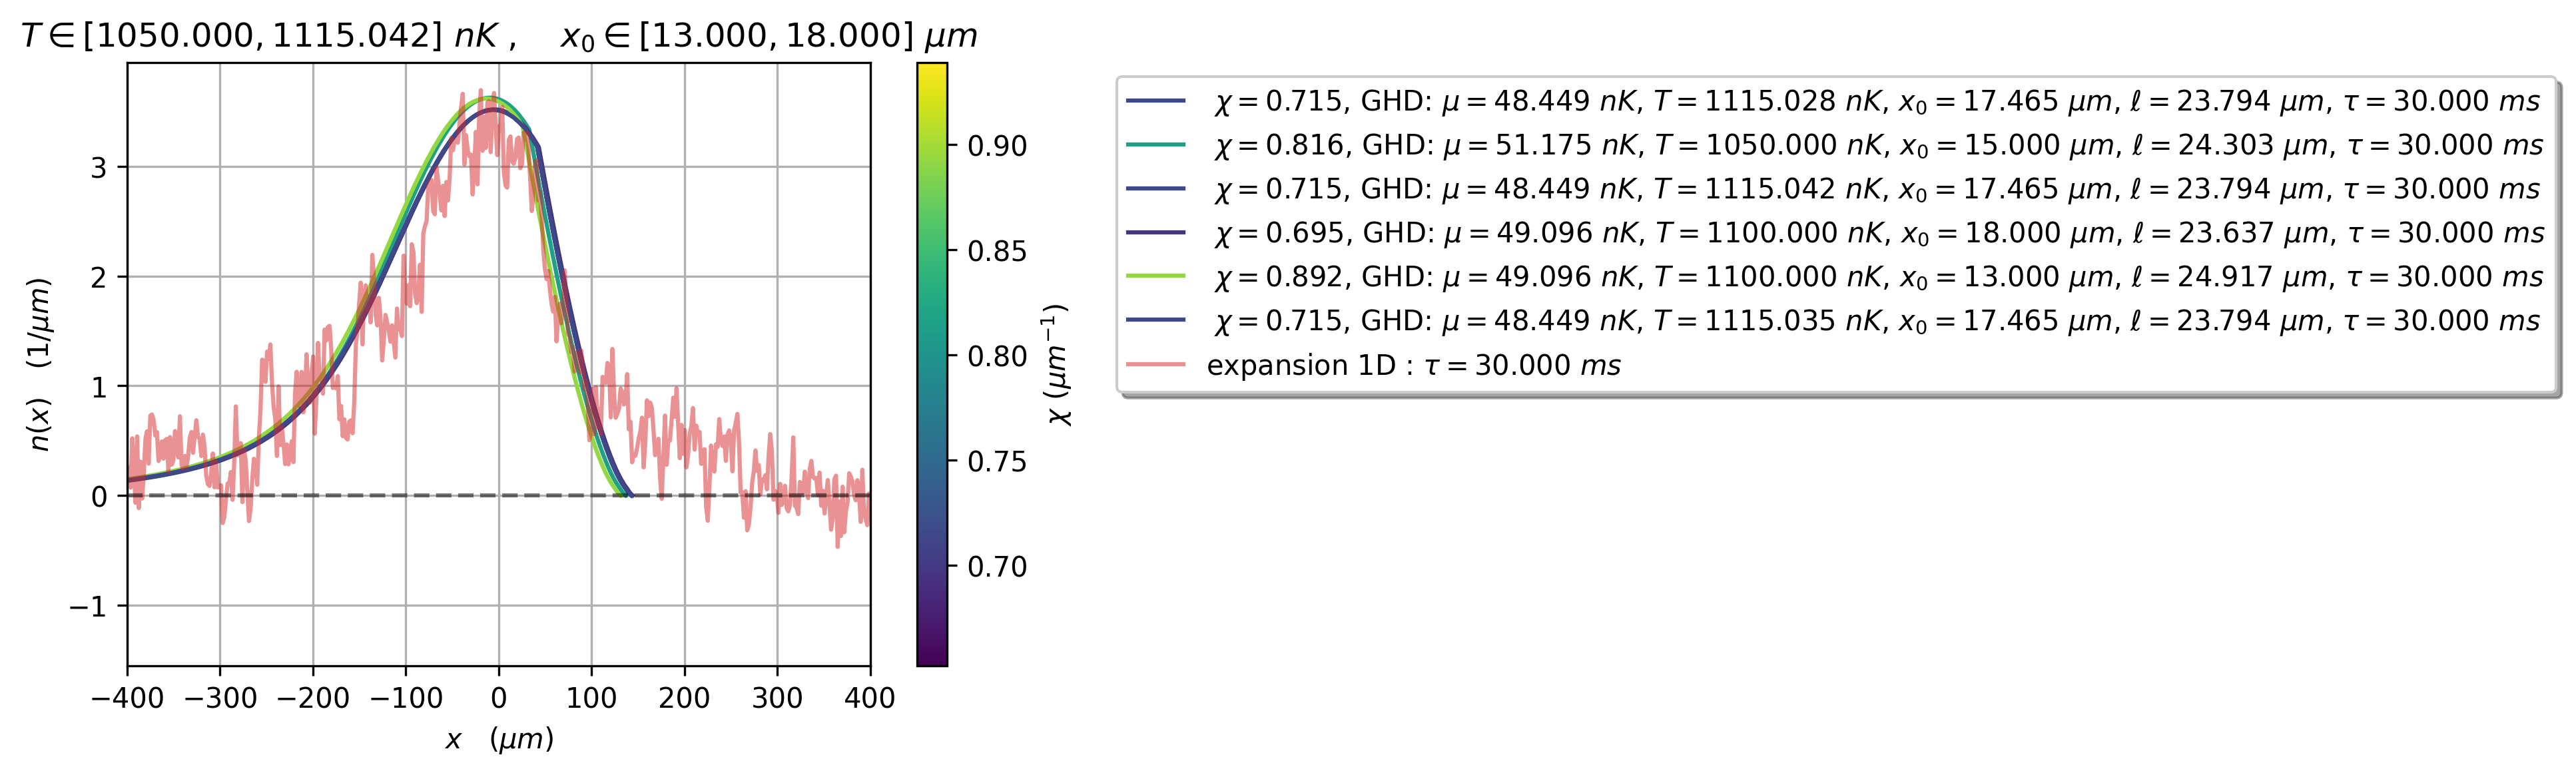
\includegraphics[width=\textwidth]{Figures/simul_expansion_T-x0-5_24-04-2024}
        \caption{}
        \label{}
    \end{subfigure}
    \vspace{1em}
    \begin{subfigure}[b]{1\textwidth}
        \centering
        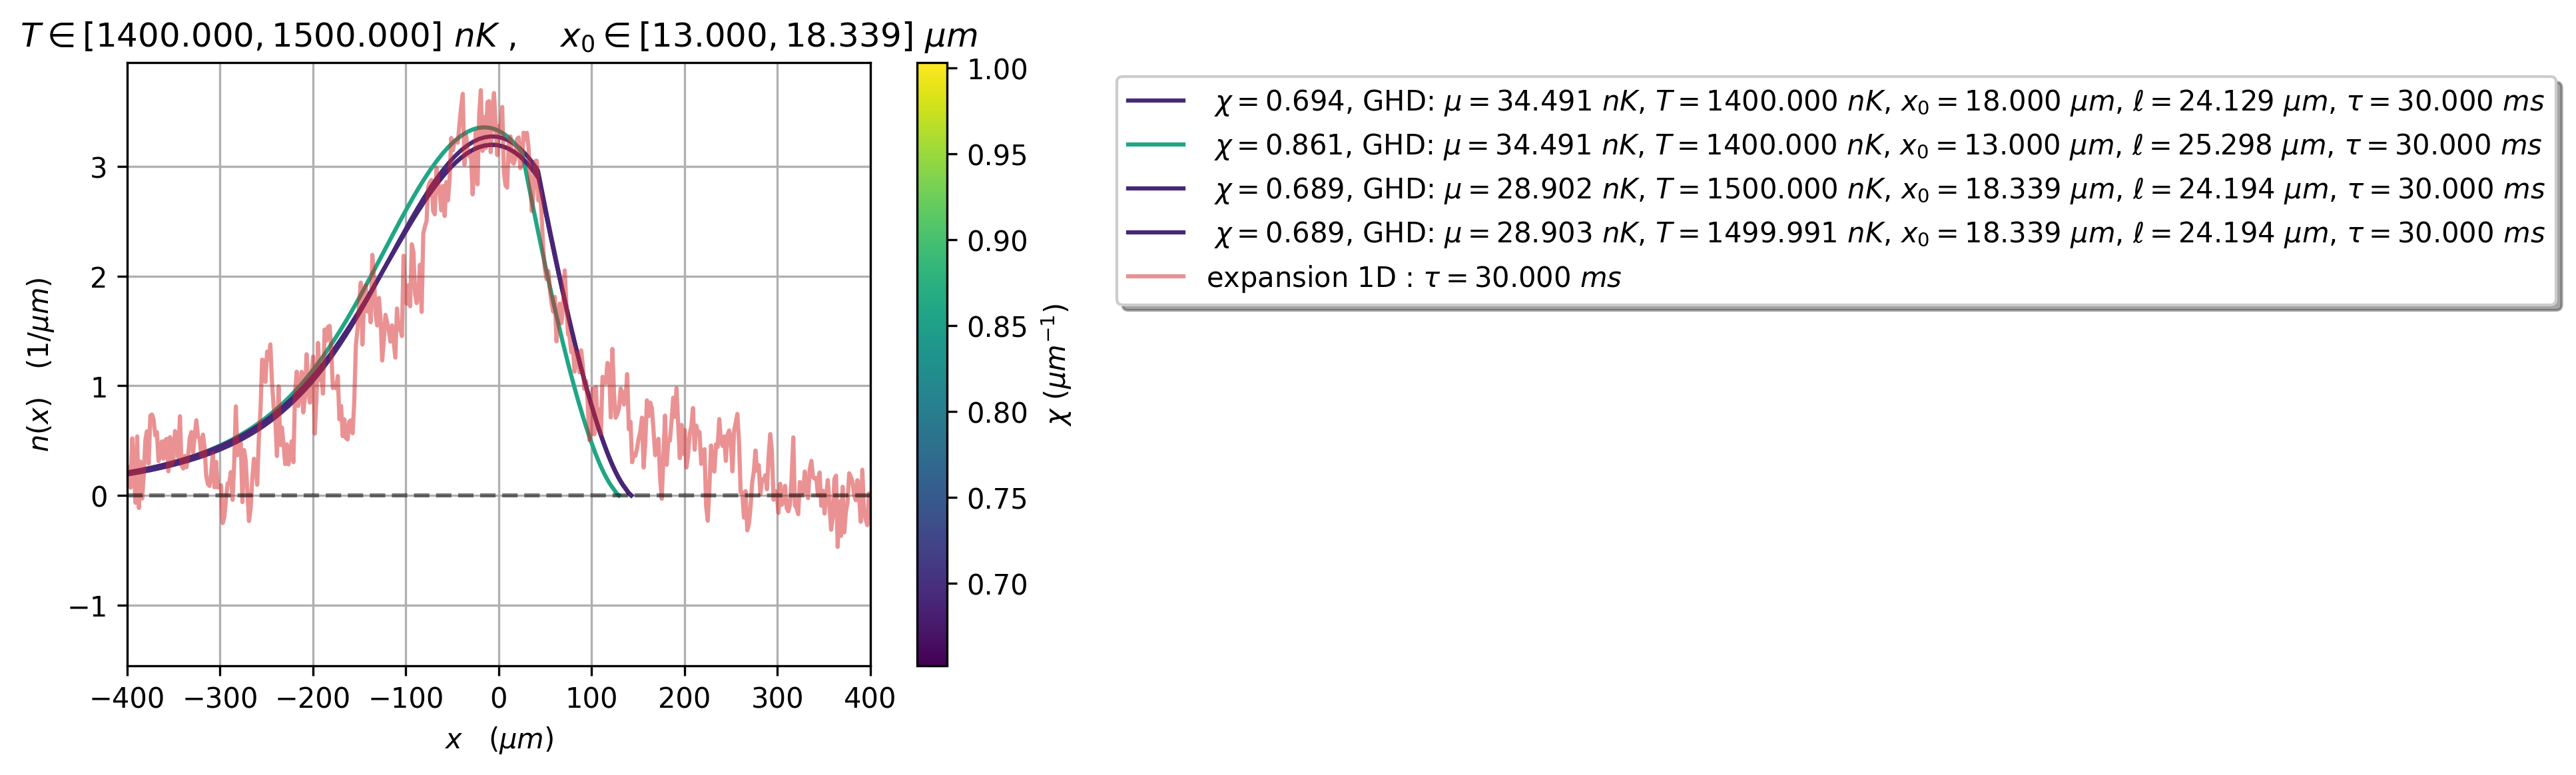
\includegraphics[width=\textwidth]{Figures/simul_expansion_T-x0-6_24-04-2024}
        \caption{}
        \label{}
    \end{subfigure}
    \vspace{1em}
    \begin{subfigure}[b]{0.48\textwidth}
        \centering
        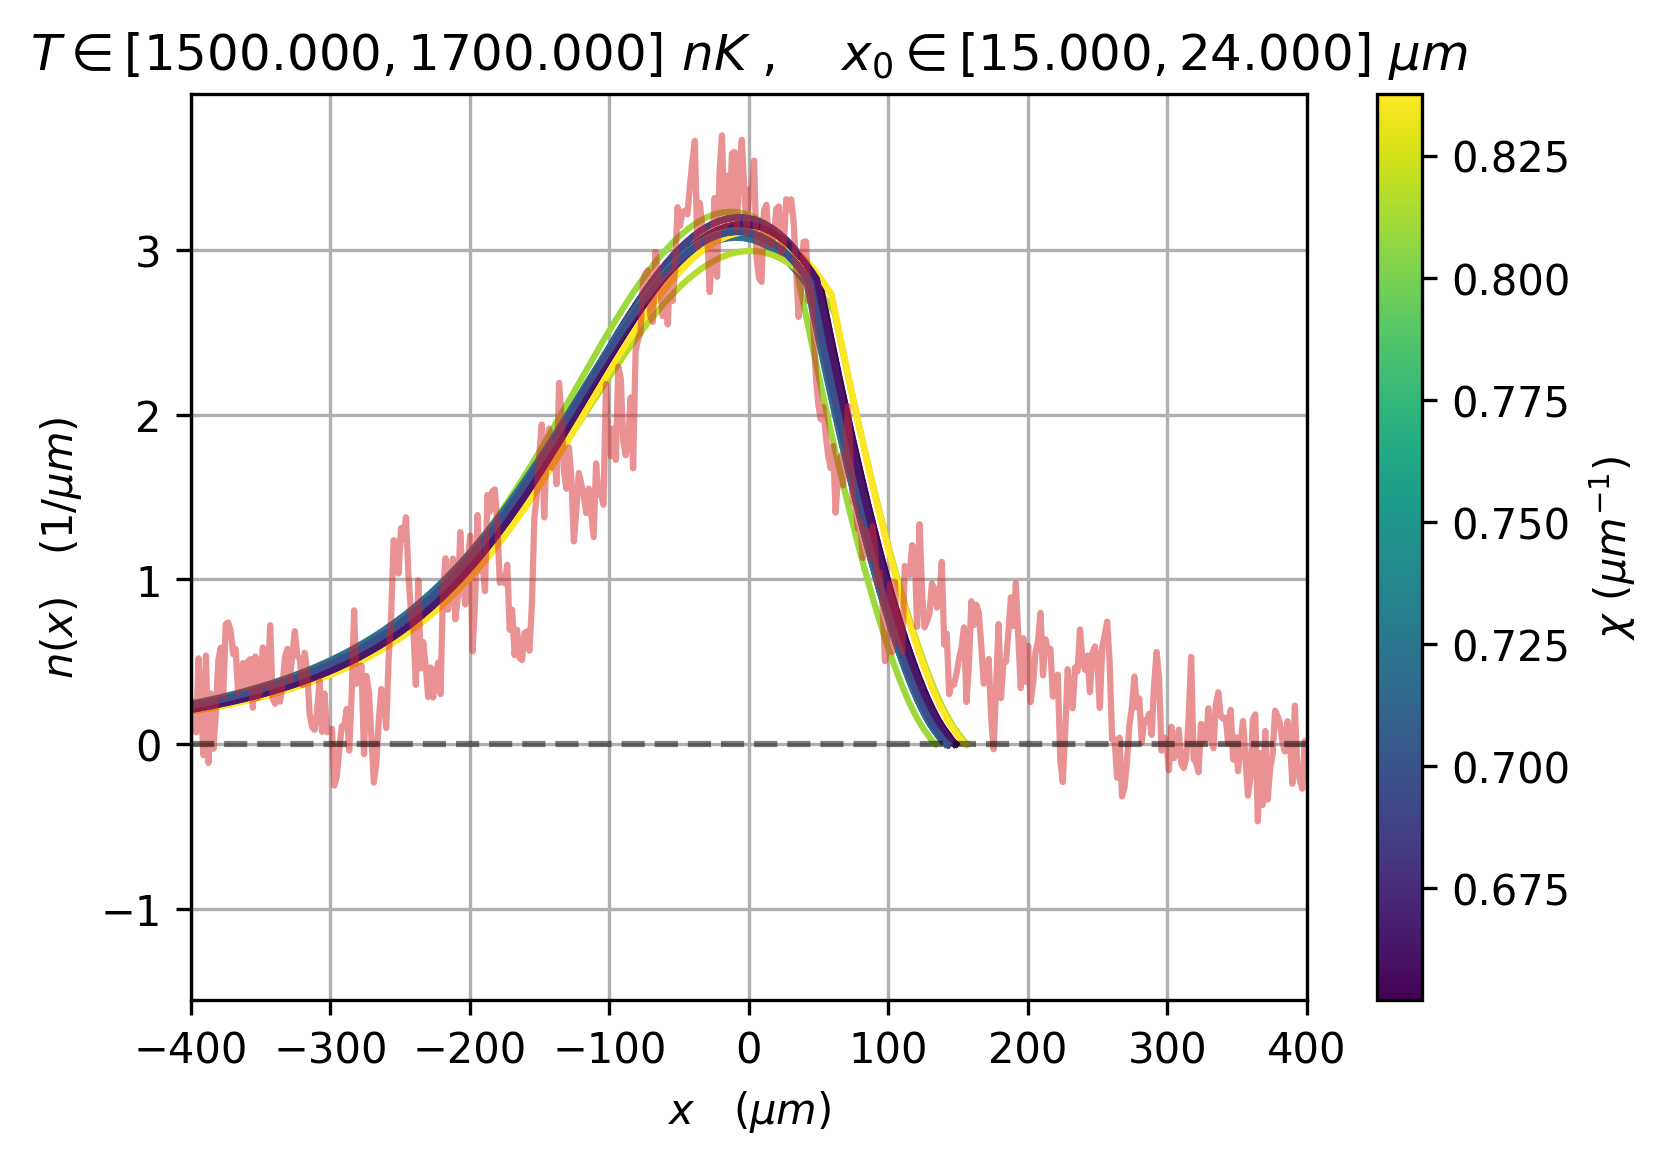
\includegraphics[width=\textwidth]{Figures/simul_expansion_T-x0-7_24-04-2024}
        \caption{}
        \label{}
    \end{subfigure}
    \hfill
	\begin{subfigure}[b]{0.48\textwidth}
        \centering
        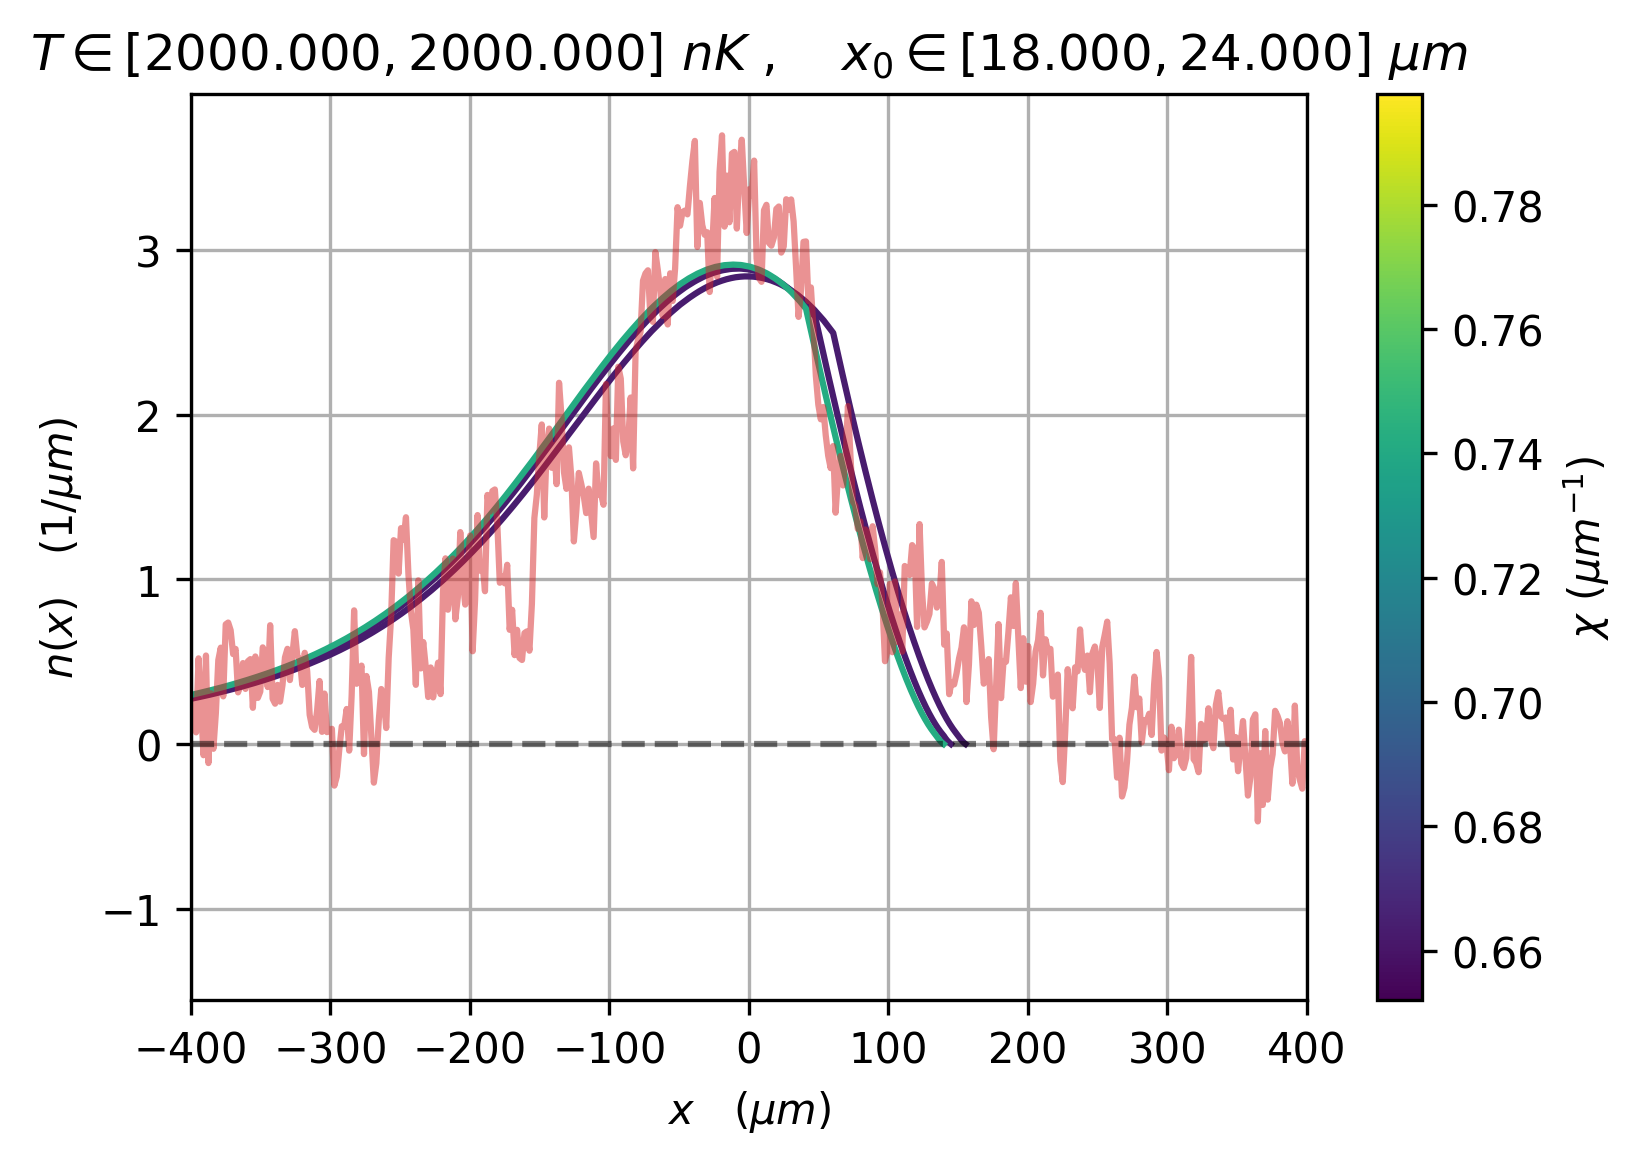
\includegraphics[width=\textwidth]{Figures/simul_expansion_T-x0-8_24-04-2024}
        \caption{}
        \label{}
    \end{subfigure}


    \caption{Donnée du 24-04-2024}
    \label{}
\end{figure}
	
	\begin{figure}[H]
	\centering

    
    \begin{subfigure}[b]{0.48\textwidth}
        \centering
        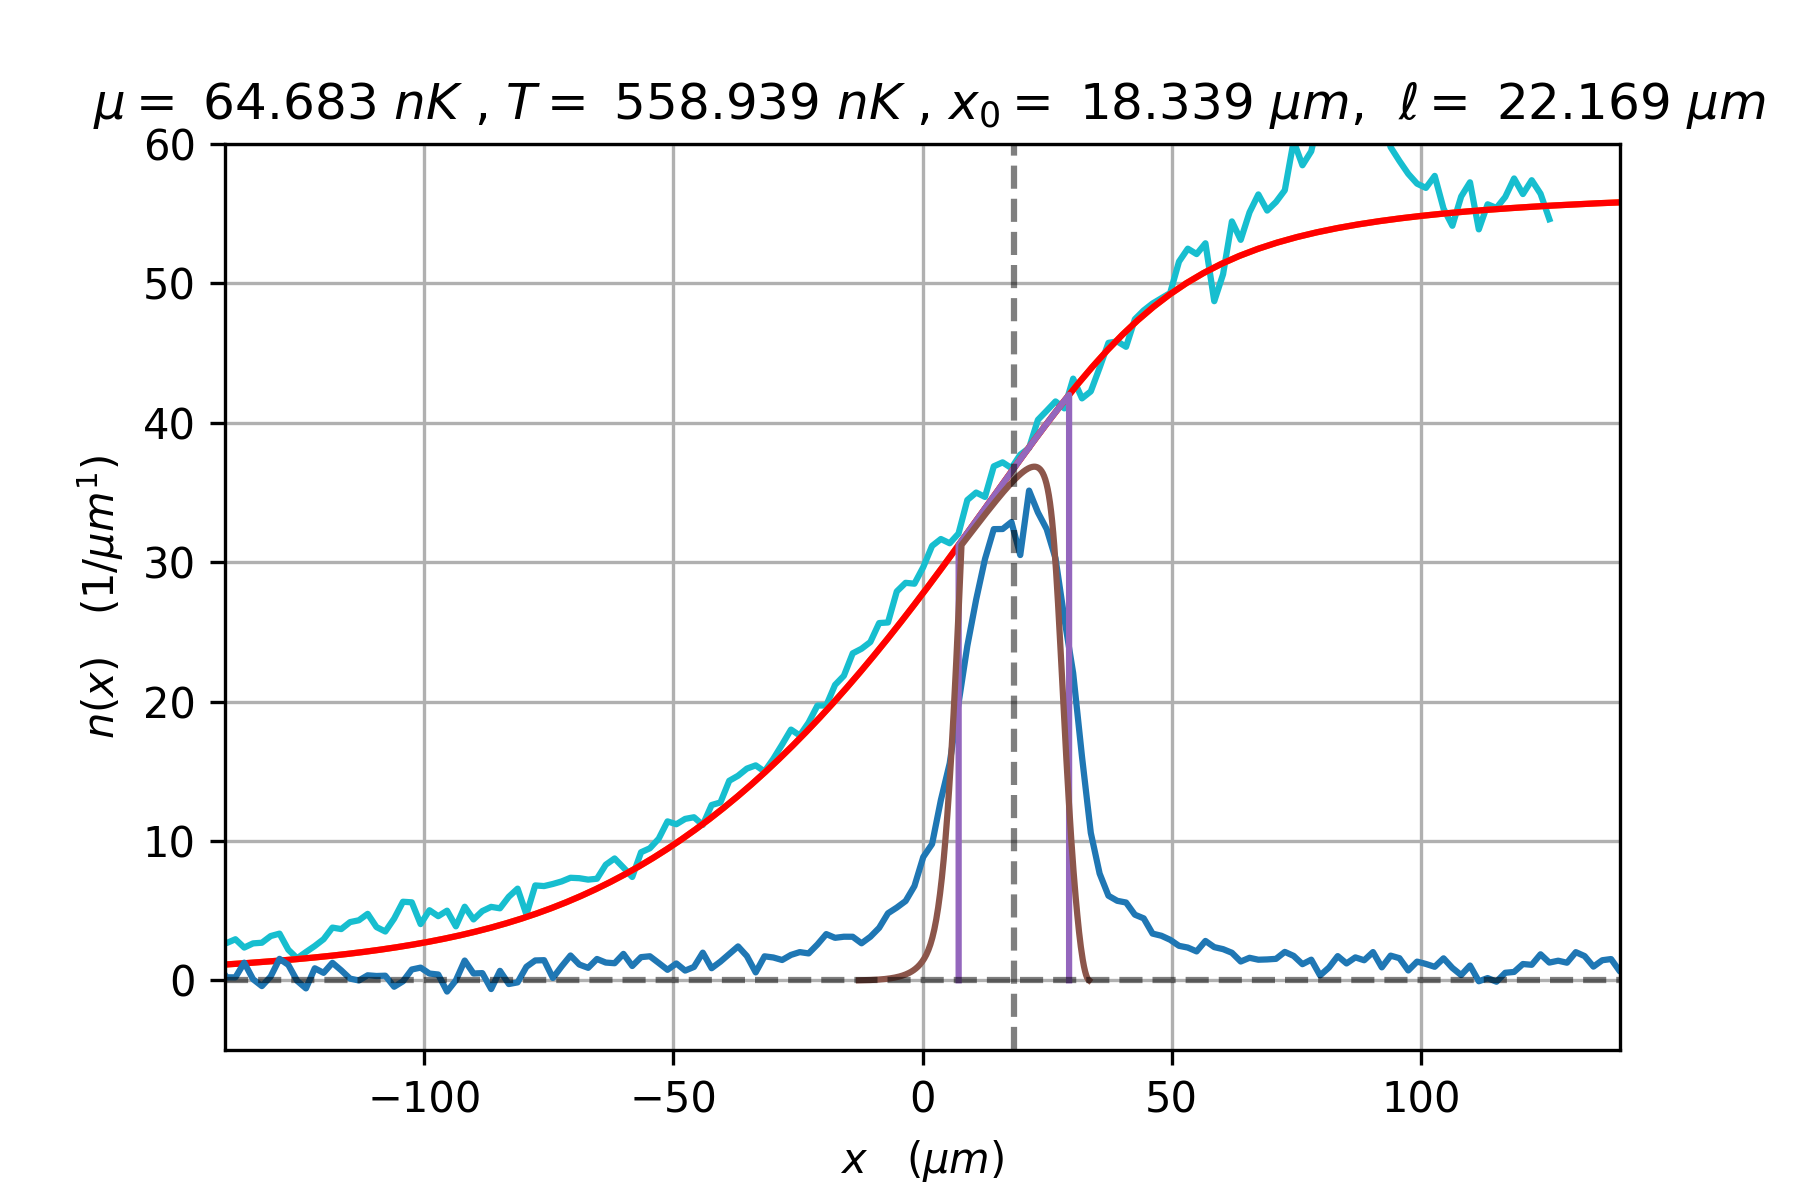
\includegraphics[width=\textwidth]{Figures/simul_deformation_1_24-04-2024}
        \caption{}
        \label{}
    \end{subfigure}
    \hfill
    \begin{subfigure}[b]{0.48\textwidth}
        \centering
        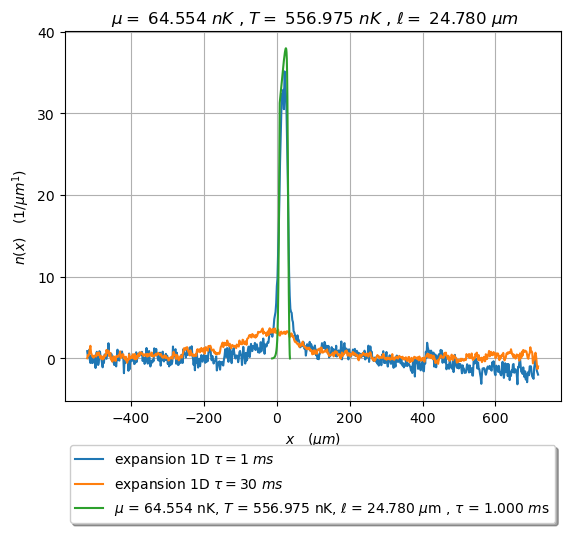
\includegraphics[width=\textwidth]{Figures/simul_expansion_1_24-04-2024}
        \caption{}
        \label{}
    \end{subfigure}
    \vspace{1em}
    \begin{subfigure}[b]{0.48\textwidth}
        \centering
        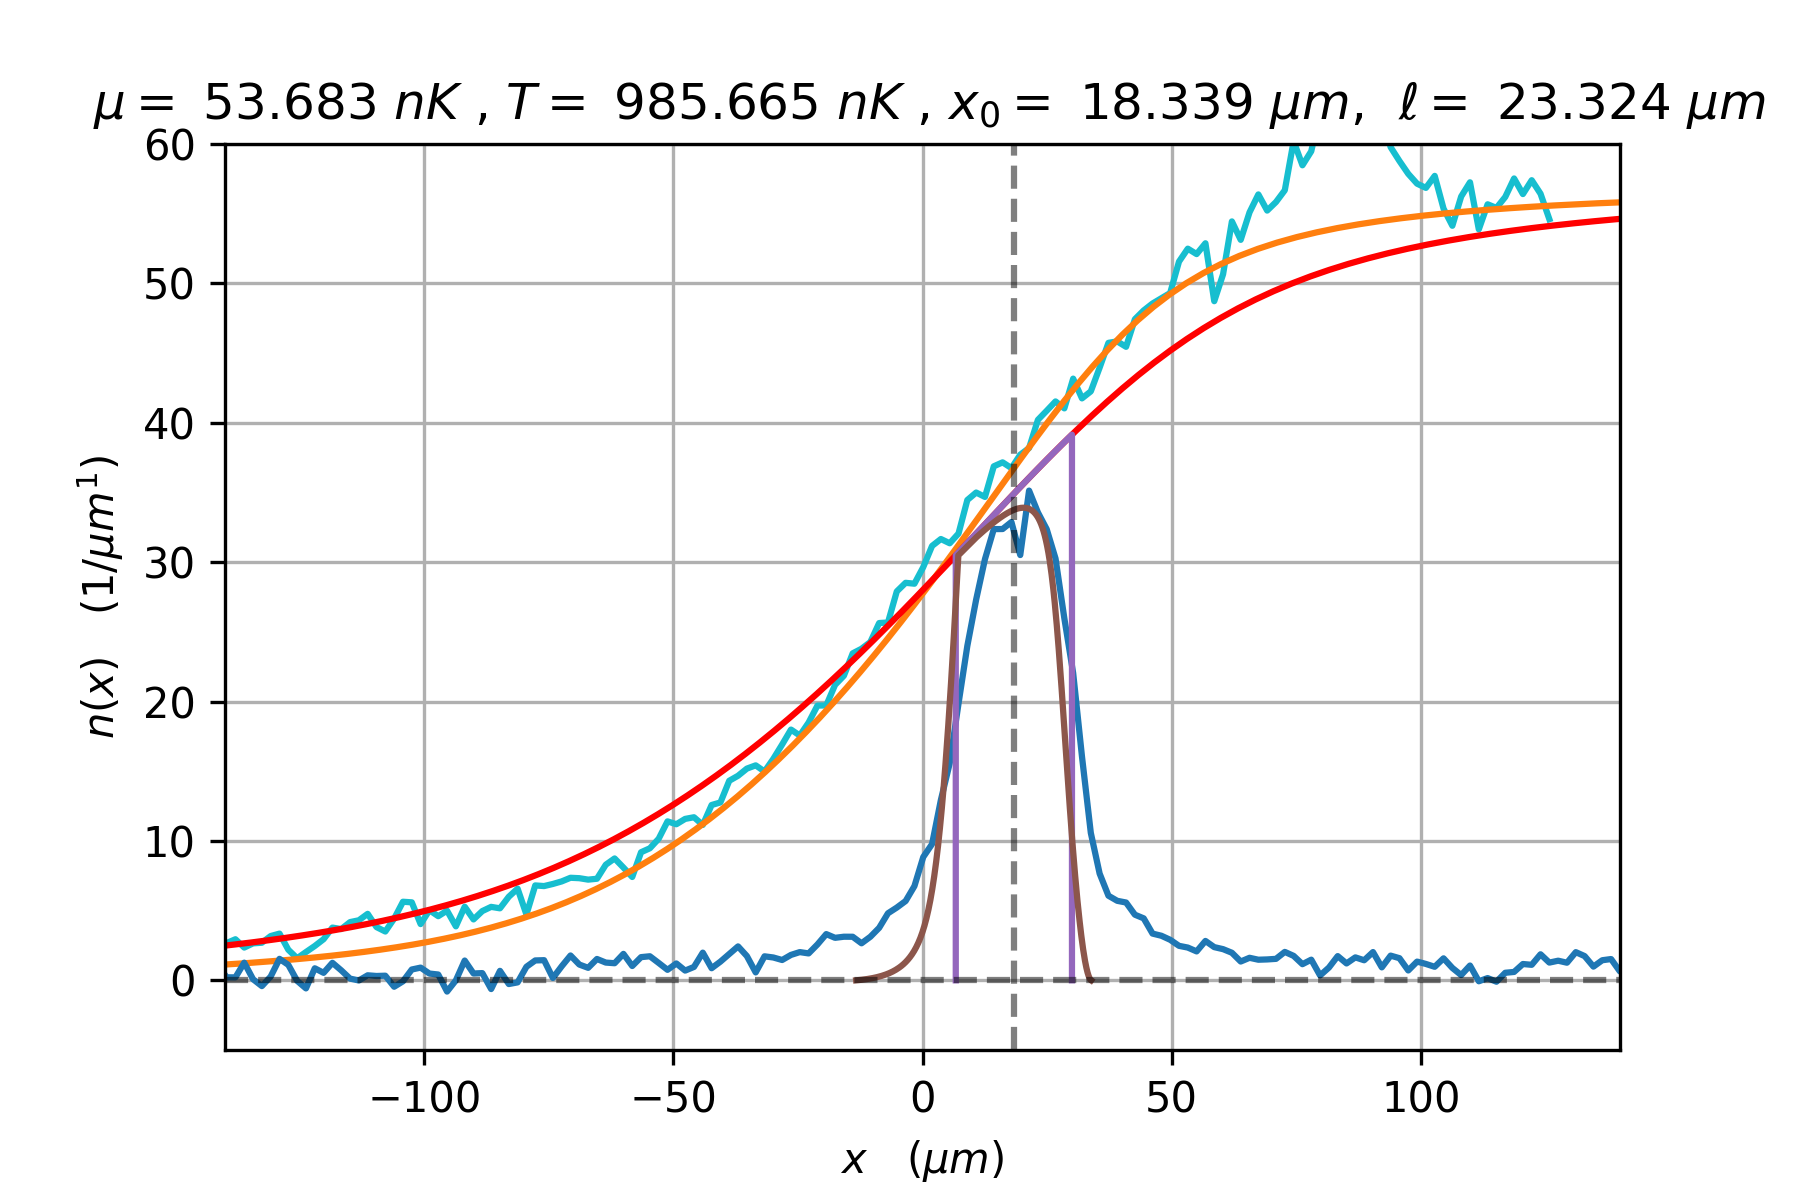
\includegraphics[width=\textwidth]{Figures/simul_deformation_2_24-04-2024}
        \caption{}
        \label{}
    \end{subfigure}
    \hfill
    \begin{subfigure}[b]{0.48\textwidth}
        \centering
        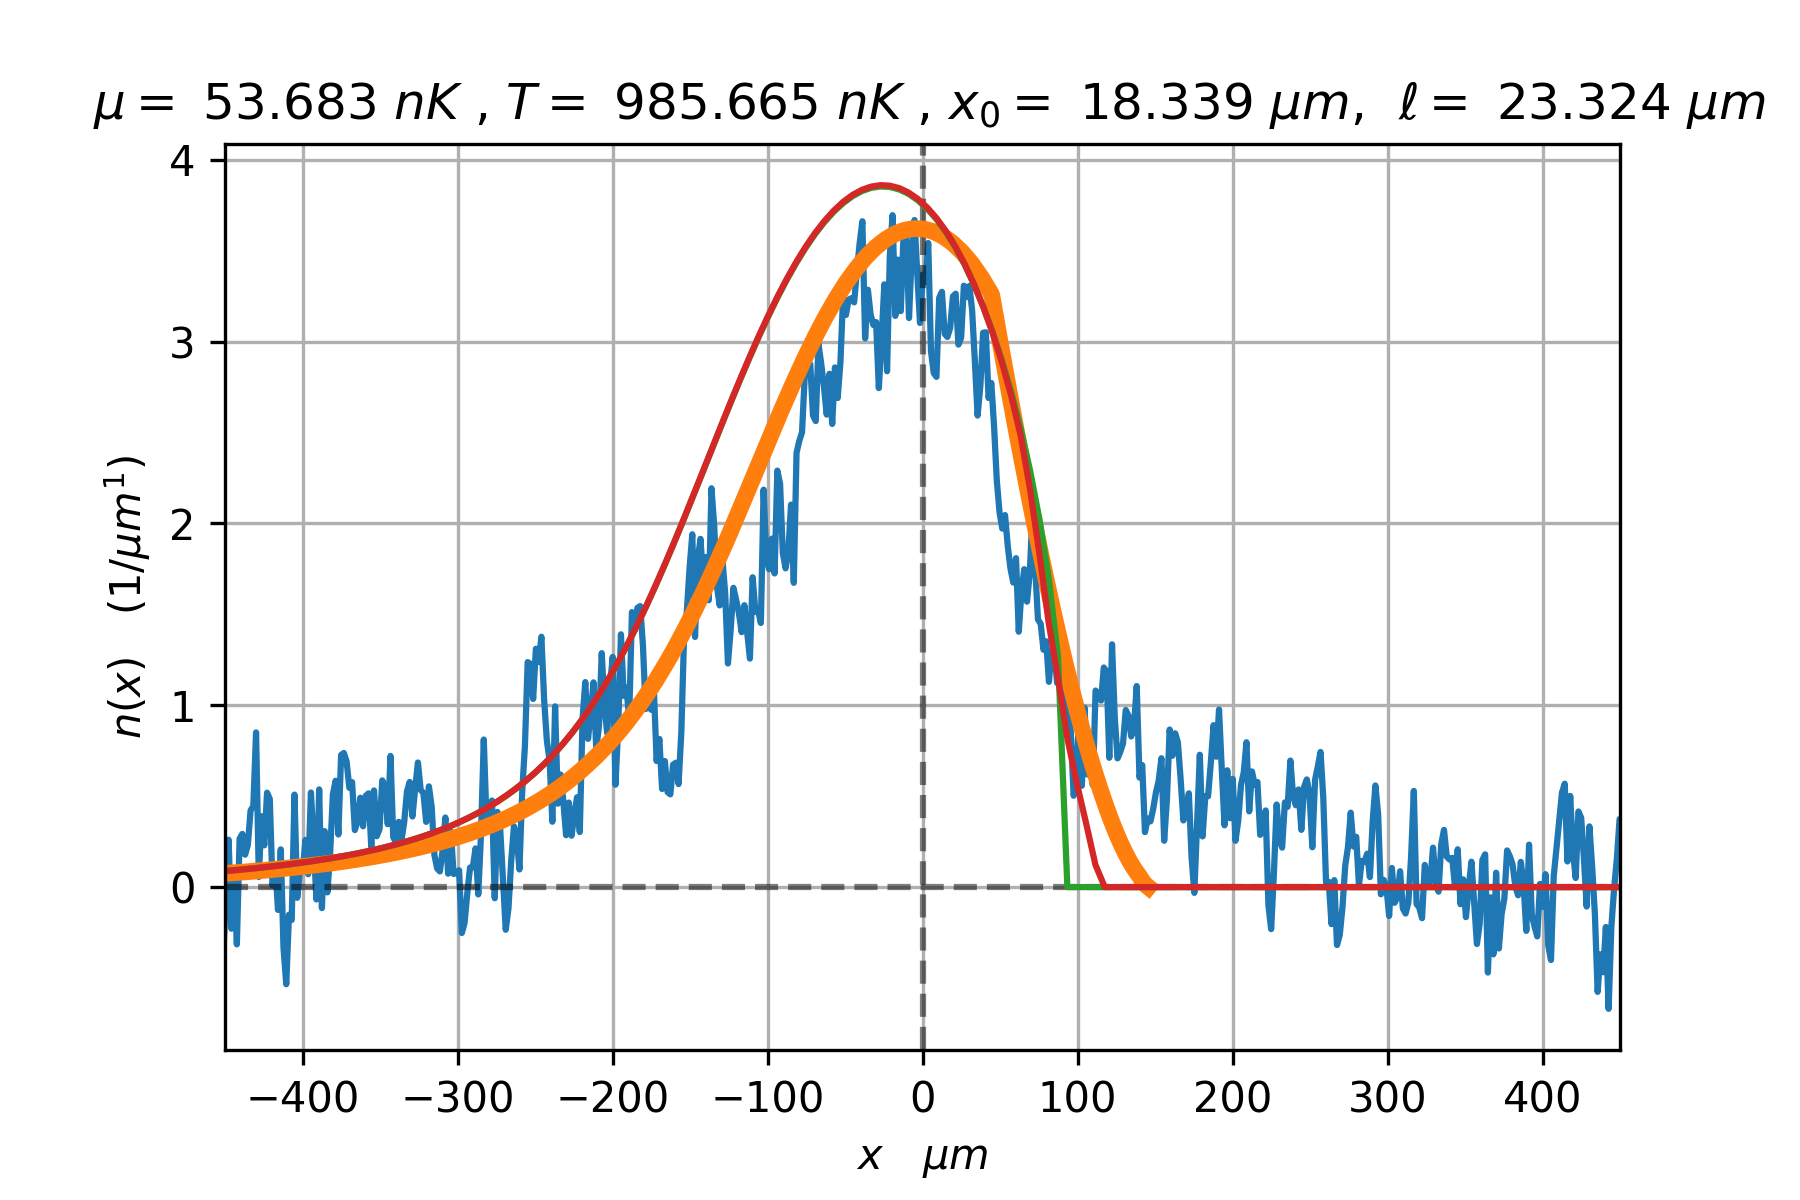
\includegraphics[width=\textwidth]{Figures/simul_expansion_2_24-04-2024}
        \caption{}
        \label{}
    \end{subfigure}
    \vspace{1em}
    \begin{subfigure}[b]{0.48\textwidth}
        \centering
        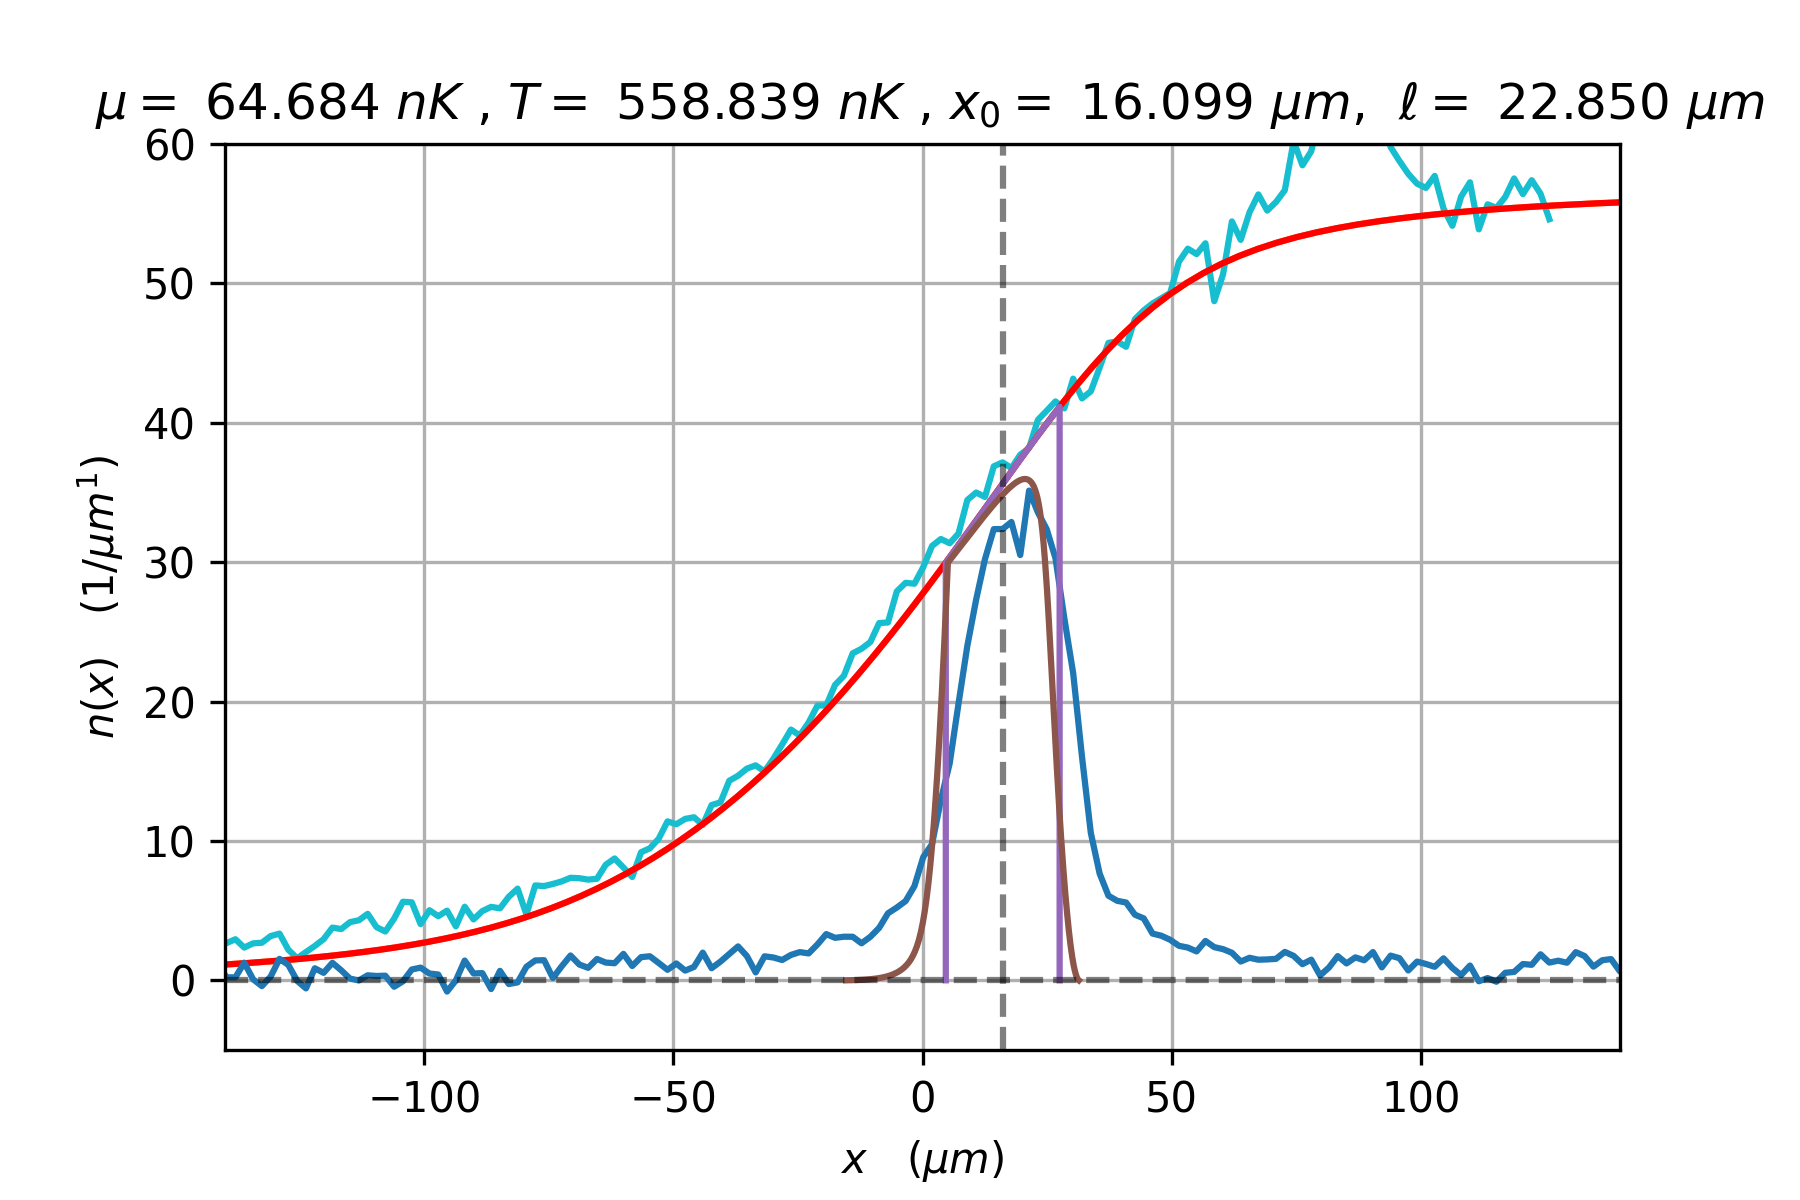
\includegraphics[width=\textwidth]{Figures/simul_deformation_3_24-04-2024}
        \caption{}
        \label{}
    \end{subfigure}
    \hfill
    \begin{subfigure}[b]{0.48\textwidth}
        \centering
        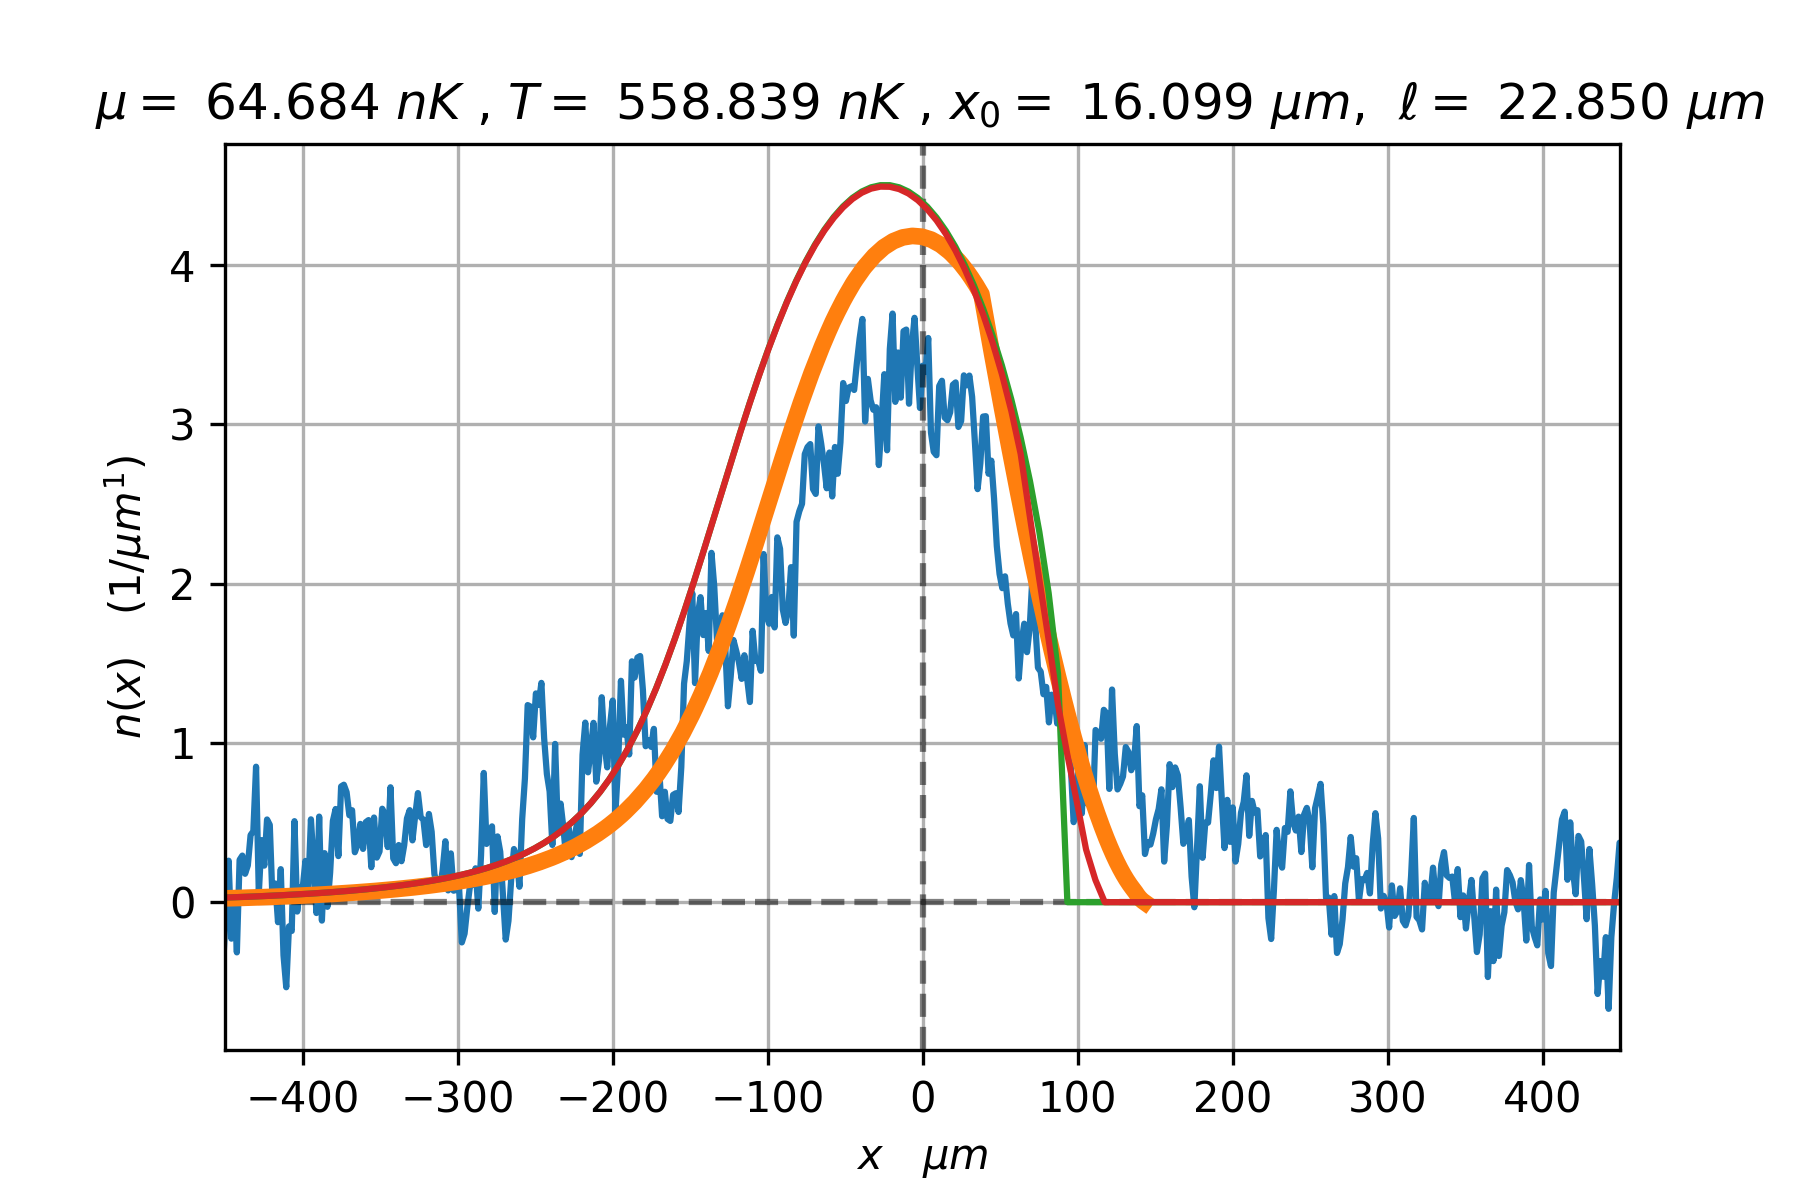
\includegraphics[width=\textwidth]{Figures/simul_expansion_3_24-04-2024}
        \caption{}
        \label{}
    \end{subfigure}
    \vspace{1em}
    \begin{subfigure}[b]{0.48\textwidth}
        \centering
        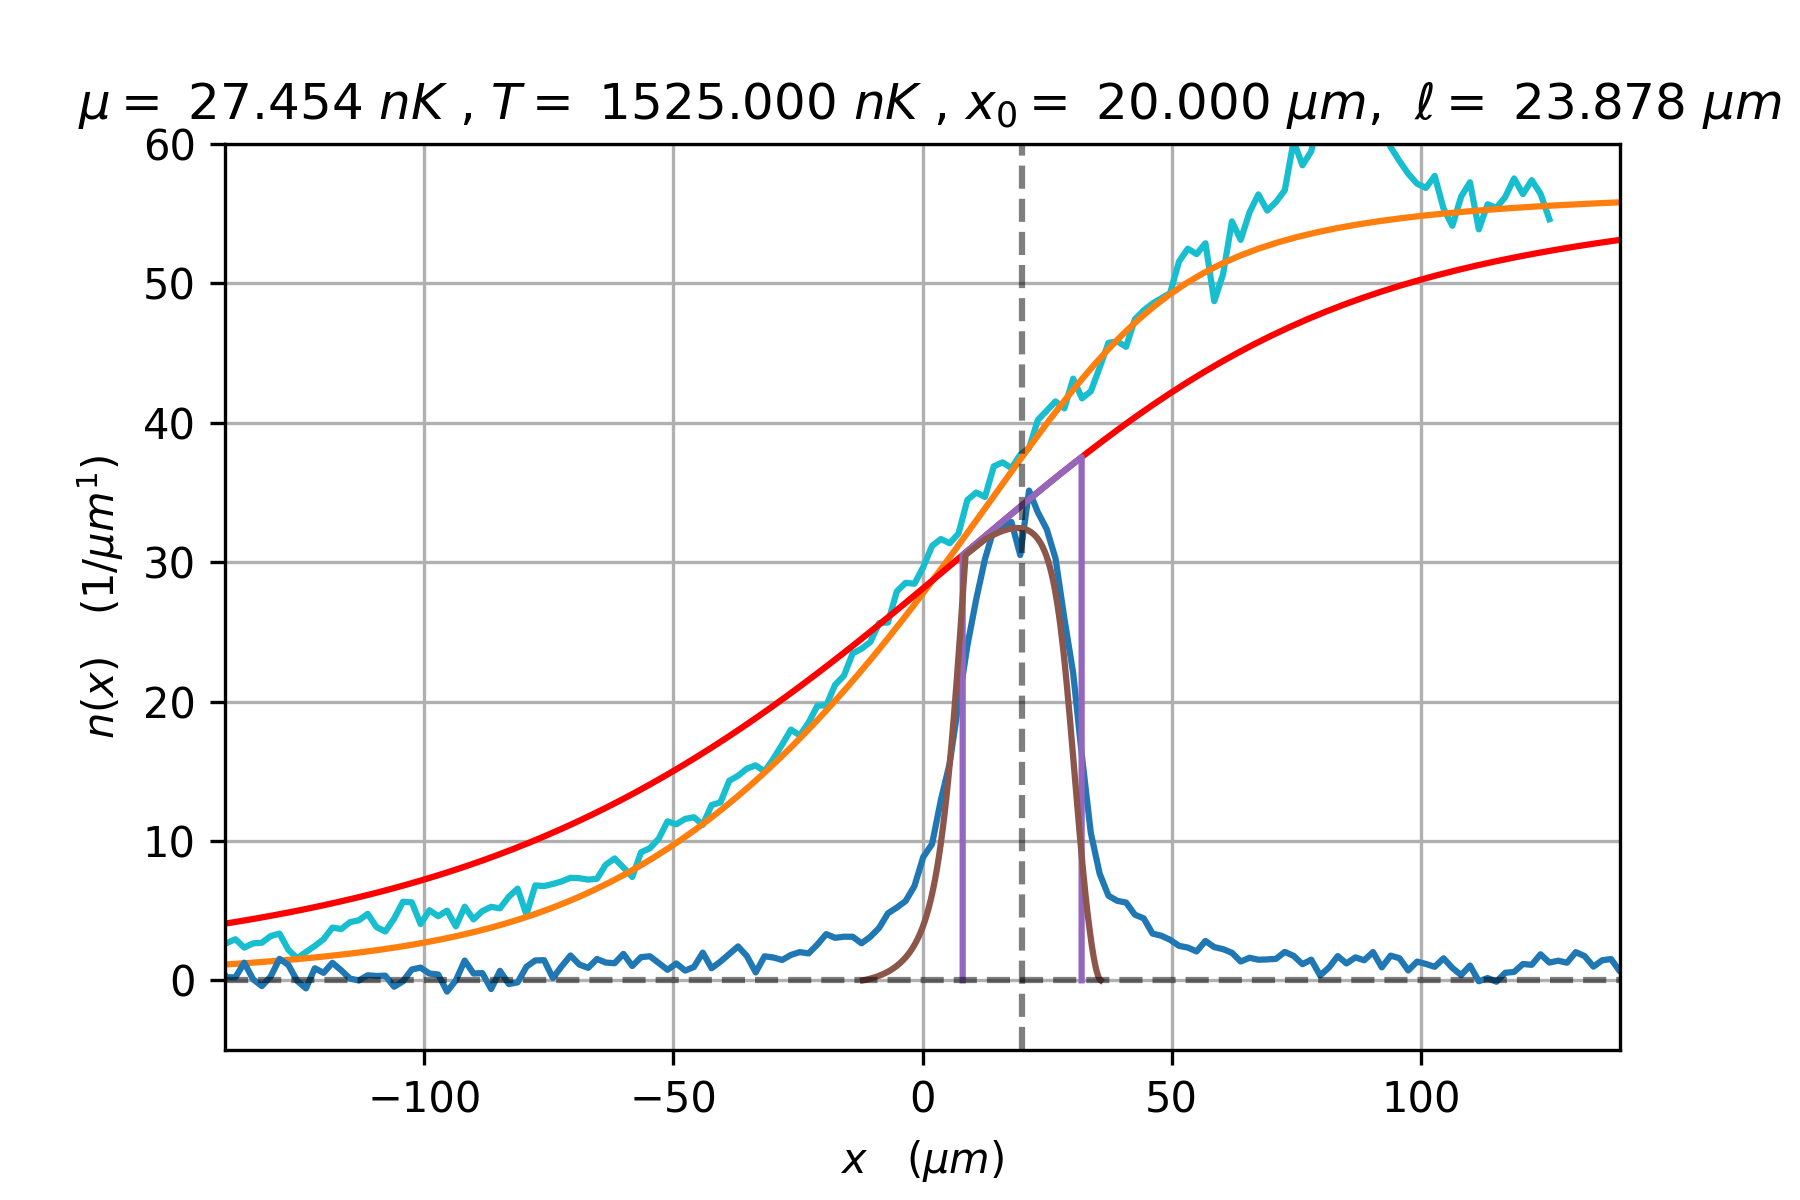
\includegraphics[width=\textwidth]{Figures/simul_deformation_4_24-04-2024}
        \caption{}
        \label{}
    \end{subfigure}
    \hfill
    \begin{subfigure}[b]{0.48\textwidth}
        \centering
        \includegraphics[width=\textwidth]{Figures/simul_expansion_4_24-04-2024}
        \caption{}
        \label{}
    \end{subfigure}

    \caption{Donnée du 24-04-2024}
    \label{}
\end{figure}

\begin{figure}[H]
\centering
	\begin{subfigure}[b]{0.48\textwidth}
        \centering
        \includegraphics[width=\textwidth]{Figures/simul_deformation_T-x0-chi-1_24-04-2024}
        \caption{}
        \label{}
    \end{subfigure}
    \hfill
    \begin{subfigure}[b]{0.48\textwidth}
        \centering
        \includegraphics[width=\textwidth]{Figures/simul_expansion_T-x0-chi-1_24-04-2024}
        \caption{}
        \label{}
    \end{subfigure}
    \vspace{1em}
    \begin{subfigure}[b]{0.48\textwidth}
        \centering
        \includegraphics[width=\textwidth]{Figures/simul_deformation_5_24-04-2024}
        \caption{}
        \label{}
    \end{subfigure}
    \hfill
    \begin{subfigure}[b]{0.48\textwidth}
        \centering
        \includegraphics[width=\textwidth]{Figures/simul_expansion_5_24-04-2024}
        \caption{}
        \label{}
    \end{subfigure}
		
\end{figure}




	\section{Essancielle}
	
	%On souhaite extraire une distribution locale de rapidité sur le bord deformé. On s'attend  
	
	%Nous commençons par faire un ajustement le profil de déformation bord avec des sumulations GDH. La temperature est le paramètre ajustable. Le potentiel chimique $\mu$ est parametrés avec la temperature $T$ et la densité initiale spatiale du nuage $n_p$. Le potentiel chimique $\mu$ est une fonctioin de $T$ et de la densité initiale spatiale du nuage $n_p$. aillant $T$ on ajuste $\mu$ pour avec un modele de thermique Yang-Yang, trouver une densité spatiale initiale de $n_p$. $n_p$ est mesuré à $56.6 ~\mu m ^{-1}$.  le meilleure ajustement de la déformation du bord est pour une temperature $T = 558.9 ~nK$ soit une potentiel chimique $\mu = 64~nK$ \ref{fig:simul_deformation}.\\
	%[Version 1]
	Nous commençons par ajuster le profil de déformation du bord en utilisant des simulations GHD, en prenant la température $T$ comme paramètre ajustable. Le potentiel chimique $\mu$ est paramétré en fonction de la température et de la densité spatiale initiale du nuage, notée $n_p$.  $\mu$  est ajusté en utilisant un modèle thermique de Yang-Yang afin de retrouver une densité spatiale initiale correspondant à $n_p$, mesurée à $56.6 ~\mu \text{m}^{-1}$. L'ajustement optimal de la déformation du bord est obtenu pour une température $T = 558.9~\text{nK}$ et un potentiel chimique $\mu = 64~\text{nK}$ (voir la Fig. \ref{fig:simul_deformation}).


	
	\begin{figure}[ht]
    \centering
    \includegraphics[width=0.5\textwidth]{Figures/simul_deformation}
    \caption{{\color{blue} [Bleu] Données de déformation du bord à $t = 18~\text{ms}$}, {\color{orange}[Orange] Ajustement avec $T = 558.939~\text{nK}$ et $\mu(T = 558.939~\text{nK}, n_p = 56.6~\mu \text{m}^{-1}) = 64.529~\text{nK}$}.}
    \label{fig:simul_deformation}
	\end{figure}

Nous souhaitons extraire une distribution locale de rapidité. Pour cela, avant de procéder à une expansion unidimensionnelle, nous sélectionnons une tranche du nuage \cite{dubois_probing_2024}. La tranche $[x_0 - \ell/2, x_0 + \ell/2[$ est celle dont nous voulons extraire la distribution de rapidité, notée $\Pi_{x_0, \ell}$. Ici, $x_0$ est le centre de la tranche et $\ell$ sa largeur.

	
		
	[Version 1.1] 
	
Pour obtenir $x_0$ et $\ell$, on ajuste, sur les données d'expansion à $\tau = 1~\text{ms}$, une fonction porte convoluée avec une gaussienne\footnote{$f(x; A, x_0, \sigma) = \frac{A}{2} \left( \operatorname{erf} \left( \frac{x + \frac{A}{2} - x_0}{\sqrt{2} \sigma} \right) - \operatorname{erf} \left( \frac{x - \frac{A}{2} - x_0}{\sqrt{2} \sigma} \right) \right)$}, où $x_0$ est le centre de la fonction et $\ell$ est la largeur à mi-hauteur\footnote{$\ell = 2\sqrt{2 \ln (2)} \sqrt{\sigma^2 + \left( \frac{A}{2} \right)^2}$}. 

On trouve $x_0 = 18.34~\mu \text{m}$ et $\ell = 33.51~\mu \text{m}$ (voir la Fig. \ref{fig:expansion_1_33}).

Ensuite, une expansion unidimensionnelle est effectuée pendant $\tau = 30~\text{ms}$. Les simulations GHD appliquées à la petite tranche donnent un profil conforme aux données (voir Fig. \ref{fig:expansion_30_33}). Après expansion, on observe une asymétrie dans les données, avec un côté plus raide. Cette asymétrie est visible dans les simulations, qui se rapprochent de la distribution de rapidité attendue, mais pas parfaitement des données.


\begin{figure}[H]
    \begin{subfigure}[b]{0.45\textwidth}
        \centering
        \includegraphics[width=\textwidth]{Figures/simul_expansion_1_33}
        \caption{{\color{blue}[Bleu] Données de sélection après expansion à $\tau = 1~\text{ms}$}, {\color{orange}[Orange] Simulation de l'expansion pour $\tau = 0~\text{ms}$, avec $x_0 = 18.4~\mu \text{m}$ et $\ell = 33.5~\mu \text{m}$, ($T = 558.9~\text{nK}$ et $\mu(T = 558.9~\text{nK}, n_p = 56.6~\mu \text{m}^{-1}) = 64.529~\text{nK}$)} et {\color{OliveGreen}[Vert] Simulation de l'expansion pour $\tau = 0~\text{ms}$, avec $x_0 = 18.4~\mu \text{m}$ et $\ell = 33.5~\mu \text{m}$, ($T = 558.9~\text{nK}$ et $\mu(T = 558.9~\text{nK}, n_p = 56.6~\mu \text{m}^{-1}) = 64.529~\text{nK}$)}}
        \label{fig:expansion_1_33}
    \end{subfigure}
    \hfill
    \begin{subfigure}[b]{0.45\textwidth}
        \centering
        \includegraphics[width=\textwidth]{Figures/simul_expansion_30_33}
        \caption{{\color{blue}[Bleu] Données expansion à $\tau = 30~\text{ms}$}, {\color{orange}[Orange] Simulation de l'expansion à $\tau = 30~\text{ms}$ avec $n_p = 56.6~\mu \text{m}^{-1}$, $T = 558.9~\text{nK}$, $\mu = 64.529~\text{nK}$, $x_0 = 18.4~\mu \text{m}$ et $\ell = 33.5~\mu \text{m}$}, {\color{OliveGreen}[Vert] Distribution de rapidité en $x = x_0$ pour $T = 558.9~\text{nK}$, $\mu = 64.529~\text{nK}$} et {\color{red}[Rouge] Distribution de rapidité dans la tranche $[x_0 - \ell/2, x_0 + \ell/2[$ pour $T = 558.9~\text{nK}$, $\mu = 64.529~\text{nK}$}}
        \label{fig:expansion_30_33}
    \end{subfigure}
    \caption{}
    \label{}
\end{figure}

[Version 1.2 ] 

	Pour déterminer $x_0$, on ajuste les données d'expansion à $\tau = 1~\text{ms}$ avec une fonction porte convoluée avec une gaussienne, où $x_0$ est le centre de la fonction. J'obtiens $x_0 = 18.34~\mu \text{m}$. Ensuite, on multiplie le profil du bord par une fonction porte centrée en $x_0$ et de diamètre $\ell$. On ajuste $\ell$ pour obtenir, dans la tranche, le même nombre d'atomes que mesuré dans les données à $\tau = 1~\text{ms}$. On trouve ainsi $\ell = 28.1~\mu \text{m}$ (voir Fig. \ref{fig:expansion_1_28}). 

Après l'expansion, on observe une asymétrie dans les données, avec un côté plus raide. Cette asymétrie est visible dans les simulations, qui sont proches de la distribution de rapidité attendue mais ne correspondent pas parfaitement aux données.

\begin{figure}[H]
    \begin{subfigure}[b]{0.45\textwidth}
        \centering
        \includegraphics[width=\textwidth]{Figures/simul_expansion_1_28}
        \caption{{\color{blue}[Bleu] Données de sélection après expansion $\tau = 1~\text{ms}$}, {\color{orange}[Orange] Simulation de l'expansion pour $\tau = 0~\text{ms}$, avec $x_0 = 18.4~\mu \text{m}$ et $\ell = 28.1~\mu \text{m}$, ($T = 558.9~\text{nK}$ et $\mu(T = 558.9~\text{nK}, n_p = 56.6~\mu \text{m}^{-1}) = 64.529~\text{nK}$)} et {\color{OliveGreen}[Vert] Simulation de l'expansion pour $\tau = 0~\text{ms}$, avec $x_0 = 18.4~\mu \text{m}$ et $\ell = 28.1~\mu \text{m}$, ($T = 558.9~\text{nK}$ et $\mu(T = 558.9~\text{nK}, n_p = 56.6~\mu \text{m}^{-1}) = 64.529~\text{nK}$)}}
        \label{fig:expansion_1_28}
    \end{subfigure}
    \hfill
    \begin{subfigure}[b]{0.45\textwidth}
        \centering
        \includegraphics[width=\textwidth]{Figures/simul_expansion_30_28}
        \caption{{\color{blue}[Bleu] Données d'expansion $\tau = 30~\text{ms}$}, {\color{orange}[Orange] Simulation de l'expansion $\tau = 30~\text{ms}$ avec $n_p = 56.6~\mu \text{m}^{-1}$, $T = 558.9~\text{nK}$, $\mu = 64.529~\text{nK}$, $x_0 = 18.4~\mu \text{m}$, et $\ell = 28.1~\mu \text{m}$}, {\color{OliveGreen}[Vert] Distribution de rapidité en $x = x_0$ pour $T = 558.9~\text{nK}$, $\mu = 64.529~\text{nK}$}, et {\color{red}[Rouge] Distribution de rapidité dans la tranche $[x_0 - \ell/2, x_0 + \ell/2 [$ pour $T = 558.9~\text{nK}$, $\mu = 64.529~\text{nK}$}}
        \label{fig:expansion_30_28}
    \end{subfigure}
    \caption{}
    \label{}
\end{figure}

	
		
	[Version 1.3 ]
	
	Pour déterminer $x_0$, on ajuste les données d'expansion à $\tau = 1~\text{ms}$ avec un modèle de fonction porte convoluée avec une gaussienne, où $x_0$ est le centre de la fonction. J'obtiens $x_0 = 18.34~\mu \text{m}$. Ensuite, on multiplie le profil de bord par une fonction porte centrée en $x_0$ et de diamètre $\ell$. On ajuste $\ell$ pour obtenir, dans la tranche, le même nombre d'atomes que mesuré dans les données à $\tau = 30~\text{ms}$. On trouve ainsi $\ell = 22.2~\mu \text{m}$ (voir Fig. \ref{fig:expansion_1_22}).

Après l'expansion, on observe une asymétrie dans les données, avec un côté plus raide. Cette asymétrie est également visible dans les simulations, qui sont proches de la distribution de rapidité attendue et des données.

\begin{figure}[H]
    \begin{subfigure}[b]{0.45\textwidth}
        \centering
        \includegraphics[width=\textwidth]{Figures/simul_expansion_1_22}
        \caption{{\color{blue}[Bleu] Données de sélection après expansion $\tau = 1~\text{ms}$}, {\color{orange}[Orange] Simulation de l'expansion pour $\tau = 0~\text{ms}$, avec $x_0 = 18.4~\mu \text{m}$ et $\ell = 22.2~\mu \text{m}$, ($T = 558.9~\text{nK}$ et $\mu(T = 558.9~\text{nK}, n_p = 56.6~\mu \text{m}^{-1}) = 64.529~\text{nK}$)} et {\color{OliveGreen}[Vert] Simulation de l'expansion pour $\tau = 0~\text{ms}$, avec $x_0 = 18.4~\mu \text{m}$ et $\ell = 22.2~\mu \text{m}$, ($T = 558.9~\text{nK}$ et $\mu(T = 558.9~\text{nK}, n_p = 56.6~\mu \text{m}^{-1}) = 64.529~\text{nK}$)}}
        \label{fig:expansion_1_22}
    \end{subfigure}
    \hfill
    \begin{subfigure}[b]{0.45\textwidth}
        \centering
        \includegraphics[width=\textwidth]{Figures/simul_expansion_30_22}
        \caption{{\color{blue}[Bleu] Données d'expansion $\tau = 30~\text{ms}$}, {\color{orange}[Orange] Simulation de l'expansion $\tau = 30~\text{ms}$ avec $n_p = 56.6~\mu \text{m}^{-1}$, $T = 558.9~\text{nK}$, $\mu = 64.529~\text{nK}$, $x_0 = 18.4~\mu \text{m}$ et $\ell = 22.2~\mu \text{m}$}, {\color{OliveGreen}[Vert] Distribution de rapidité en $x = x_0$ pour $T = 558.9~\text{nK}$, $\mu = 64.529~\text{nK}$} et {\color{red}[Rouge] Distribution de rapidité dans la tranche $[x_0 - \ell/2, x_0 + \ell/2[$ pour $T = 558.9~\text{nK}$, $\mu = 64.529~\text{nK}$}}
        \label{fig:expansion_30_22}
    \end{subfigure}
    \caption{}
    \label{}
\end{figure}

	 
	
	
	{\color{blue} centre bouge entre $\tau = 0$ et $\tau = 1~ms$ et mon mesure une diference de 17$\%$ de nombre d'atome sentre $\tau = 1~ms$ et $\tau = 30 ~ms$ sur les données d'expension}
	
	
	[Version 1.4.1]
	
	La tranche a une dynamique moyenne. Donc  les donnée etais prisent après un temps d'expansion $\tau$ de 1ms, on ne sais pas directement où est le centre  $x_0$ et la taille $\ell$ de la tranche.
	On peut faire un ajustement des simulation GHD sur le profile à une temps d'expansion $\tau$ de 1ms. .....
	
	[Version 1.4.2]	
	
	La tranche a une dynamique moyenne. Donc  les donnée etais prisent après un temps d'expansion $\tau$ de 1ms, on ne sais pas directement où est le centre  $x_0$ et la taille $\ell$ de la tranche.
	On peut faire un ajustement des simulation GHD sur le profile à une temps d'expansion $\tau$ de 30ms. .....
	
	\begin{figure}[H]
    \begin{subfigure}[b]{0.32\textwidth}
        \centering
        \includegraphics[width=\textwidth]{Figures/simul_expansion_30_expansion_0}
        \caption{}
        \label{}
    \end{subfigure}
    \hfill
    \begin{subfigure}[b]{0.32\textwidth}
        \centering
        \includegraphics[width=\textwidth]{Figures/simul_expansion_30_expansion_09}
        \caption{}
        \label{fig:expansion_1_expansion}
    \end{subfigure}
    \hfill
    \begin{subfigure}[b]{0.32\textwidth}
        \centering
        \includegraphics[width=\textwidth]{Figures/simul_expansion_30_expansion_15}
        \caption{}
        \label{}
    \end{subfigure}
    
    \vspace{1em}
    
     \begin{subfigure}[b]{0.32\textwidth}
        \centering
        \includegraphics[width=\textwidth]{Figures/simul_expansion_30_expansion_18}
        \caption{}
        \label{}
    \end{subfigure}
    \hfill
    \begin{subfigure}[b]{0.32\textwidth}
        \centering
        \includegraphics[width=\textwidth]{Figures/simul_expansion_30_expansion_21}
        \caption{}
        \label{fig:expansion_1_expansion}
    \end{subfigure}
    \hfill
    \begin{subfigure}[b]{0.32\textwidth}
        \centering
        \includegraphics[width=\textwidth]{Figures/simul_expansion_30_expansion_23}
        \caption{}
        \label{}
    \end{subfigure}
    
    \vspace{1em}
    
    \begin{subfigure}[b]{0.32\textwidth}
        \centering
        \includegraphics[width=\textwidth]{Figures/simul_expansion_30_expansion_28}
        \caption{}
        \label{}
    \end{subfigure}
    \hfill
    \begin{subfigure}[b]{0.32\textwidth}
        \centering
        \includegraphics[width=\textwidth]{Figures/simul_expansion_30_expansion_23}
        \caption{}
        \label{fig:expansion_1_expansion}
    \end{subfigure}
    \hfill
    \begin{subfigure}[b]{0.32\textwidth}
        \centering
        \includegraphics[width=\textwidth]{Figures/simul_expansion_30_expansion_36}
        \caption{}
        \label{}
    \end{subfigure}
    
    
    
    \caption{}
    


    
    \label{}
\end{figure}
	
	
	[Version 2]
	
	%Nous voulons extraire une distribution locale de rapidités. Pour cela nous commençons par sélectionner une tranche $[x_0 - \ell/2 , x_0 + \ell/2 [ $ du bord. Puis nous faisons une expansion undimensionnele pendant une durée $\tau$ de $30~ms$. 
	
	Nous avons des données d'expansion unidimensionnel pour $\tau = 1~ms$ et $\tau = 30~ms$. La tranche as une dynamique moyenne pendant $1~ms$ et les atomes hors de la tranche n'ont pas eu le temps de completement sortir du piège donc on ne peut pas ni extraire directement le centre de la trance $x_0$, ni la largeur de la tranche $\ell$ sur nos donnée d'expansion à $\tau = 1~ms$. Pour ce faire , on a supposer que pendant $1~ms$ le centre de la tranche n'a pas bouger. En faisant un ajustement gaussien des donnée à $\tau = 1 ~ ms$ , on trouve un centre $x_0 = 18.339~\mu m$. Sur l'ajustement du bord  on a ajuste $\ell$ pour que ne nombre d'atome mesuré dans la tranche sois la même  que mesuré dans sur les donnés à un temps d'expansion $\tau = 30~ms$. On trouve ainsi $\ell = 22.2~\mu \text{m}$ (voir Fig. \ref{fig:simul_deformation_expansion})
	
	\begin{figure}[H]
    \begin{subfigure}[b]{0.32\textwidth}
        \centering
        \includegraphics[width=\textwidth]{Figures/simul_deformation_expansion}
        \caption{{\color{blue} [Bleu] Données de déformation du bord à $t = 18~\text{ms}$},{\color{orange}[Orange] Ajustement avec $T = 558.939~\text{nK}$ et $\mu(T = 558.939~\text{nK}, n_p = 56.6~\mu \text{m}^{-1}) = 64.529~\text{nK}$}, {\color{OliveGreen}[Vert] Simulation de l'expansion pour $\tau = 0~\text{ms}$, avec $x_0 = 18.339~\mu \text{m}$ et $\ell = 22.176~\mu \text{m}$, ($T = 558.9~\text{nK}$ et $\mu(T = 558.9~\text{nK}, n_p = 56.6~\mu \text{m}^{-1}) = 64.529~\text{nK}$)}.}
        \label{fig:simul_deformation_expansion}
    \end{subfigure}
    \hfill
    \begin{subfigure}[b]{0.32\textwidth}
        \centering
        \includegraphics[width=\textwidth]{Figures/simul_expansion_1_expansion}
        \caption{{\color{orange}[Orange] Ajustement avec $T = 558.939~\text{nK}$ et $\mu(T = 558.939~\text{nK}, n_p = 56.6~\mu \text{m}^{-1}) = 64.529~\text{nK}$}, {\color{red}[Rouge] Ajustement avec $T = ~\text{nK}$ et $\mu(T = ~\text{nK}, n_p = 56.6~\mu \text{m}^{-1}) = ~\text{nK}$}, {\color{blue}[Vert] Données de sélection après expansion $\tau = 1~\text{ms}$}, {\color{orange}[Orange] Simulation de l'expansion pour $\tau = 0~\text{ms}$, avec $x_0 = 18.4~\mu \text{m}$ et $\ell = ~\mu \text{m}$, ($T = 558.9~\text{nK}$ et $\mu(T = ~\text{nK}, n_p = 56.6~\mu \text{m}^{-1}) = ~\text{nK}$)}, {\color{violet}[Violet] Simulation de l'expansion pour $\tau = 0~\text{ms}$, avec $x_0 = 18.4~\mu \text{m}$ et $\ell = ~\mu \text{m}$, ($T = ~\text{nK}$ et $\mu(T = ~\text{nK}, n_p = 56.6~\mu \text{m}^{-1}) = ~\text{nK}$)}et {\color{brown}[Marron] Simulation de l'expansion pour $\tau = 1~\text{ms}$, avec $x_0 = 18.4~\mu \text{m}$ et $\ell = ~\mu \text{m}$, ($T = ~\text{nK}$ et $\mu(T = ~\text{nK}, n_p = 56.6~\mu \text{m}^{-1}) = ~\text{nK}$)}.}
        \label{fig:simul_deformation_expansion}
    \end{subfigure}
    \hfill
    \begin{subfigure}[b]{0.32\textwidth}
        \centering
        \includegraphics[width=\textwidth]{Figures/simul_expansion_30_expansion}
        \caption{{\color{blue}[Bleu] Données d'expansion $\tau = 30~\text{ms}$}, {\color{orange}[Orange] Simulation de l'expansion $\tau = 30~\text{ms}$ avec $n_p = 56.6~\mu \text{m}^{-1}$, $T = ~\text{nK}$, $\mu = ~\text{nK}$, $x_0 = 18.4~\mu \text{m}$ et $\ell = 22.2~\mu \text{m}$}, {\color{OliveGreen}[Vert] Distribution de rapidité en $x = x_0$ pour $T = ~\text{nK}$, $\mu = ~\text{nK}$} et {\color{red}[Rouge] Distribution de rapidité dans la tranche $[x_0 - \ell/2, x_0 + \ell/2[$ pour $T = ~\text{nK}$, $\mu = ~\text{nK}$}}
        \label{fig:expansion_30_expansion}
    \end{subfigure}
    \caption{}
    \label{}
\end{figure}
	
	
	\begin{figure}[H]
    \begin{subfigure}[b]{0.32\textwidth}
        \centering
        \includegraphics[width=\textwidth]{Figures/simul_deformation_expansion1}
        \caption{{\color{blue} [Bleu] Données de déformation du bord à $t = 18~\text{ms}$}, {\color{orange}[Orange] Ajustement avec $T = ~\text{nK}$ et $\mu(T = ~\text{nK}, n_p = 56.6~\mu \text{m}^{-1}) = ~\text{nK}$}.}
        \label{fig1:simul_deformation_expansion}
    \end{subfigure}
    \hfill
    \begin{subfigure}[b]{0.32\textwidth}
        \centering
        \includegraphics[width=\textwidth]{Figures/simul_expansion_1_expansion1}
        \caption{{\color{blue}[Bleu] Données de sélection après expansion $\tau = 1~\text{ms}$}, {\color{orange}[Orange] Simulation de l'expansion pour $\tau = 0~\text{ms}$, avec $x_0 = 18.4~\mu \text{m}$ et $\ell = ~\mu \text{m}$, ($T = 558.9~\text{nK}$ et $\mu(T = ~\text{nK}, n_p = 56.6~\mu \text{m}^{-1}) = ~\text{nK}$)} et {\color{OliveGreen}[Vert] Simulation de l'expansion pour $\tau = 0~\text{ms}$, avec $x_0 = 18.4~\mu \text{m}$ et $\ell = ~\mu \text{m}$, ($T = ~\text{nK}$ et $\mu(T = ~\text{nK}, n_p = 56.6~\mu \text{m}^{-1}) = ~\text{nK}$)}}
        \label{fig1:expansion_1_expansion}
    \end{subfigure}
    \hfill
    \begin{subfigure}[b]{0.32\textwidth}
        \centering
        \includegraphics[width=\textwidth]{Figures/simul_expansion_30_expansion1}
        \caption{{\color{blue}[Bleu] Données d'expansion $\tau = 30~\text{ms}$}, {\color{orange}[Orange] Simulation de l'expansion $\tau = 30~\text{ms}$ avec $n_p = 56.6~\mu \text{m}^{-1}$, $T = ~\text{nK}$, $\mu = ~\text{nK}$, $x_0 = 18.4~\mu \text{m}$ et $\ell = 22.2~\mu \text{m}$}, {\color{OliveGreen}[Vert] Distribution de rapidité en $x = x_0$ pour $T = ~\text{nK}$, $\mu = ~\text{nK}$} et {\color{red}[Rouge] Distribution de rapidité dans la tranche $[x_0 - \ell/2, x_0 + \ell/2[$ pour $T = ~\text{nK}$, $\mu = ~\text{nK}$}}
        \label{fig1:expansion_30_expansion}
    \end{subfigure}
    \caption{}
    \label{}
\end{figure}

	
	
	
	
	
	
	
	\begin{figure}[h]
        \centering
		%\includegraphics[width=1\textwidth]{Figures/Shema.pdf}
	\caption{les profiles du 24-04-2024 : }
        \label{fig:donnes}
    \end{figure}
    
    
    
	\section{Les données } 
	
	\begin{minipage}[b]{0.45\textwidth} 
    \begin{itemize}
        \item[Date :] 2024-04-24
        \item[Scan :] 89-97-102-108
        \item[Paramètres :] With1, DeadtimeDMD, With1\_bis, DeadtimeDMD\_bis
    \end{itemize}

    \vspace{1em} % Espacement entre la liste et la figure
    
    %\begin{figure}[ht]
        \centering
        \includegraphics[width=0.8\textwidth]{Figures/donnees_24-04-2024} % Remplacez par le chemin correct de l'image
        \captionof{figure}{Les profils du 24-04-2024}
        %\label{fig:donnes}
    %\end{figure}

    \vspace{1em} % Espacement entre la figure et la liste d'énumération
    
    \begin{enumerate}[label=\alph*)]
        {\color{blue} \item \color{blue} "Deformation bord $\tau = 1~ms$" (\ref{fig:donnes}) : Profil longitudinal des données $1~ms$ après la sélection en $x = 0$.}
        {\color{orange}\item "Deformation bord $\tau = 18~ms$" (\ref{fig:donnes}) : Profil longitudinal des données après $18~ms$ de déformation du bord.}
        {\color{\OliveGreen} \item "Expansion 1D $\tau = 1~ms$" (\ref{fig:donnes}) : Profil longitudinal des données après $1~ms$ d'expansion.}
        {\color{red} \item "Expansion 1D $\tau = 30~ms$" (\ref{fig:donnes}) : Profil longitudinal des données après $30~ms$ d'expansion.}
    \end{enumerate}
  \end{minipage}
  \hfill % Espacement flexible entre les deux minipages
	\begin{minipage}[b]{0.45\textwidth}
			
	\begin{enumerate}[label =\Alph*)]

		\item Système semi-infinie pour $x\geq 0$ :
			\begin{enumerate}[label =\alph*)]
				\item Système dans une potentiel quartique  :
					\begin{itemize}[label =$\bullet$]
						\item fréquence transverse : $\omega_\perp \overset{exp}{=} 2 \pi * 2.56 ~KHz$	
						\item la densité spatial: $n_0 = n_p $  sur les données {\color{blue} "deformation bord $\tau = 1~ ms$" (\ref{fig:donnes}), je mesure   $n_p \overset{exp}{=} 56.6 ~{\mu m}^{-1}$.}
					\end{itemize}
				\item Selection de $x\geq 0$  :
					\begin{itemize}[label =$\bullet$]
						%\item[$\circ$] le graphe ("deformation bord $\tau = 1~ ms$ (\ref{fig:donnes})) représente le profile longitudinale des données $1 ~ms$ aprés la selection en $x = 0$ 
						\item la densité spatial théorique : $n_0 = n_p \Theta (x) $  
						\item garde le potentiel transverse
					\end{itemize}

			\end{enumerate}
			
			 
		\item Deformation du bord : 
			\begin{itemize}[label =$\bullet$]
				\item[$\circ$] "deformation bord $\tau = 1~ ms$ (\ref{fig:donnes}) : le profile longitudinale des données apres $1~ms$ de déformation du bord
				\item[$\circ$] "deformation bord $\tau = 18~ ms$ (\ref{fig:donnes}) : le profile longitudinale des données apres $18~ms$ de déformation du bord
				\item garde le potentiel transverse %$\omega_\perp \overset{exp}{=} 2 \pi * 2.56 ~KHz$
				\item temps de déformation du bord $\tau = 18~ ms$	
			\end{itemize}
		\item Mesure locale de distribution de rapidité , Expansion 1D   : 
			\begin{enumerate}[label =\alph*)]
				\item Local : selection de la tranche $[ x_0 - \ell/2 , x_0 + \ell/2 [$:
					\begin{itemize}[label =$\bullet$]
						\item $x_0 = 19.6 ~\mu m $ (trouvé avec un ajustement gaussien sur "expansion 1D $\tau =1~ms$" (\ref{fig:donnes}) ) 
						\item $\ell = 24.78 ~ \mu m $ (trouvé en faisant la différence des positions des extremums du gradient de s données "expansion 1D $\tau =1~ms$" (\ref{fig:donnes}) ) 	
					\end{itemize}
				\item Expansion :
					\begin{itemize}[label =$\bullet$]
						\item[$\circ$] "expansion 1D $\tau =1~ms$" : profile longitudinale des données après $1~ms$ d'expansion.
						\item[$\circ$] "expansion 1D $\tau =30~ms$" : profile longitudinale des données après $30~ms$ d'expansion.
						\item temps de déformation du bord $\tau = 18~ ms$		
					\end{itemize}
				\item[$\bullet$] garde le potentiel transverse %$\omega_\perp \overset{exp}{=} 2 \pi * 2.56 ~KHz$


			\end{enumerate}
			

	\end{enumerate}
	
	\end{minipage}
	
	\section{Simulation GHD}

	
		\subsection{Méthode 1 (Ajustement sur la déformation du bord ($\mu( T , n_p = 56.6 ~{\mu m}^{-1} ) , T , x_0 = 19.6 ~\mu m  , \ell = 24.78 ~ \mu m  $ ): } 
		
		
		
		\begin{figure}[H]
			\begin{subfigure}[b]{0.45\textwidth}
        		\centering
        		\includegraphics[width=\textwidth]{Figures/simul_deformation_18_24-04-2024}
        		\caption{{\color{blue} [Bleu] Donnée de Déformation du bord $t= 18 ~ms$},{\color{OliveGreen}[ Vert ]  Ajustement avec $T = 556.975 ~nK$ et $\mu ( T =556.975 ~nK  , n_p = 56.6 ~{\mu m}^{-1} )= 64.554~nK$}, {\color{orange}[Orange] Donnée de Selection après expansion $\tau = 1~ms$} et {\color{red}[Rouge] Simulation de l'expansion pour $\tau= 1~ms$  , avec $x_0 = 19.6~\mu m$ et $\ell = 24.78~\mu m$ }  }
        		\label{fig:ajustementdeform}
    		\end{subfigure}
    		\hfill
    		\begin{subfigure}[b]{0.45\textwidth}
        		\centering
        		\includegraphics[width=\textwidth]{Figures/simul_expansion_1_24-04-2024}
        		\caption{{\color{blue}[Bleu] Donnée de Selection après expansion $\tau = 1~ms$}, {\color{OliveGreen}[Vert]  Simulation de l'expansion pour $\tau= 1~ms$  , avec $x_0 = 19.6~\mu m$ et $\ell = 24.78~\mu m$ et ($T = 556.975 ~nK$ et $\mu=556.975 ~nK  , n_p = 56.6 ~{\mu m}^{-1} )= 64.554~nK$)} et { \color{orange}[Orange] Données de l'expansion pour $\tau = 30~ms$  } }
        		\label{fig:expansion1}
    		\end{subfigure}
    		
    		\vspace{1em}
    		
     		\begin{subfigure}[b]{0.45\textwidth}
        		\centering
        		\includegraphics[width=\textwidth]{Figures/simul_expansion_30_24-04-2024}
        		\caption{{\color{blue}[Bleu] Donnée  expansion $\tau = 30~ms$} , {\color{orange}[Orange] Simulation de  expansion $\tau = 30~ms$ avec $n_p = 56.6 ~{\mu m}^{-1}$ , $T = 556.975 ~nK$ , $\mu=556.975 ~nK$ , $x_0 = 19.6~\mu m$ , et $\ell = 24.78~\mu m$} et {\color{\OliveGreen}[Vert] Distribution de rapidité en $x = 0$ pour  $T = 556.975 ~nK$ , $\mu=556.975 ~nK$} }
        		\label{fig:expansion30}
    		\end{subfigure}
    		\hfill
    		\begin{subfigure}[b]{0.45\textwidth}
        		\centering
        		\includegraphics[width=\textwidth]{Figures/Nat}
        		\caption{{\color{blue}[Bleu] Déviation de du nombre d'atome simulé par raport au nombre d'atome simulé à $\tau = 0 ~ms$ } , {\color{orange}[Orange] Déviation de du nombre d'atome simulé par rapport au nombre d'atome mesuré dans les donné à $\tau = 1 ~ms$} ,  {\color{\OliveGreen}[Vert] Déviation de du nombre d'atome simulé par raport au nombre d'atome mesuré sur les donné à $\tau = 30 ~ms$} et {\color{red}[Rouge] Déviation de du nombre d'atome mesurer sur les donné à $\tau = 30 ~ms$ rapport au nombre d'atome mesuré sur les donné à $\tau = 1 ~ms$} }
        		\label{fig:nat}
    		\end{subfigure}
				
		\end{figure}
		
			\begin{enumerate}[label =\Alph*)]
				


				
				\item Ajustement sur la déformation du bord (\ref{fig:ajustementdeform}):

					\begin{enumerate}[label =\alph*)]
						\item On extrais la temperature $T$ en faisant un ajustement sur le profil de bord 
						\item Le potentiel chimique est une fonction de la temperature $T$ et la densité $n_p$ : $\mu( T , n_p = 56.6 ~{\mu m}^{-1} )$ tel que $\int \rho_{ [ \nu_{\{T,\mu\}} ] } (\theta) \, d \theta  = n_p $ 
						\item[$\circ$] L'ajustement donne $T = 556.975 ~nK$ et $\mu( T=556.975 ~nK , n_p = 56.6 ~{\mu m}^{-1} ) = 64.554~nK $ 
					\end{enumerate}
					
				\item Selection $[ x_0 - \ell/2 , x_0 + \ell/2[$ 
					\begin{itemize}
								\item[$\circ$] $x_0 = 19.6 ~\mu m $ (trouvé avec un ajustement gaussien sur {\color{OliveGreen}"expansion 1D $\tau =1~ms$" (\ref{fig:donnes})} ou {\color{orange} (\ref{fig:ajustementdeform}) } ou {\color{blue}(\ref{fig:expansion1})} ) 
								\item[$\circ$] $\ell = 24.78 ~ \mu m $ (trouvé en faisant la différence des positions des extremums du gradient des données {\color{OliveGreen}"expansion 1D $\tau =1~ms$" (\ref{fig:donnes})} ou {\color{orange} (\ref{fig:ajustementdeform}) } ou {\color{blue}(\ref{fig:expansion1})} )
							\end{itemize}
				\item Expansion 
					\begin{itemize}
								\item[$\bullet$]	 On considère que la tranche $[ x_0 - \ell/2 , x_0 + \ell/2[$ n'est pas homogène 
								\item[$\circ$] Après Simulation GHD on obtiens les profil {\color{orange} orange de \ref{fig:expansion30}}  
									\begin{itemize}
										\item Les simulations GHD Conservent le nombre d'atoms à $3\%$ près ({\color{blue} blue de \ref{fig:nat}})
										\item Les simulations GHD de l'expansion commencent avec une erreur $10\%$ en nombre d'atome par rapport au nombre d'atome mesuré les données d'expansion à $\tau = 1~ms$ ({\color{orange} Premier point de la courbe orange de \ref{fig:nat}}) 
										\item Les simulations GHD de l'expansion se terminent avec une erreur $13\%$ en nombre d'atome par rapport au nombre d'atome mesuré les données d'expansion $\tau = 30~ms$ ({\color{\OliveGreen} Dernier point de la courbe verte de \ref{fig:nat}})
										\item Les mesures sur les données du nombre d'atomes lors de l'expansion montrent une perte de $17\%$ du nombre d'atomes ({\color{red} rouge \ref{fig:nat}})
									\end{itemize}	 	
							\end{itemize}

			\end{enumerate}
			
			
\subsection{Méthode 1.1 (Ajustement sur la déformation du bord + ajustement $x_0$ et $\ell$ ($\mu( T , n_p = 56.6 ~{\mu m}^{-1} ) , T , x_0 = 18.852 ~\mu m  , \ell = 27.860 ~ \mu m  $ ): } 
		
		
		
		\begin{figure}[H]
			\begin{subfigure}[b]{0.45\textwidth}
        		\centering
        		\includegraphics[width=\textwidth]{Figures/simul_deformation_18_24-04-2024-1.1.png}
        		\caption{{\color{blue} [Bleu] Donnée de Déformation du bord $t= 18 ~ms$},{\color{OliveGreen}[ Vert ]  Ajustement avec $T = 558.939 ~nK$ et $\mu ( T =558.939 ~nK  , n_p = 56.6 ~{\mu m}^{-1} )= 64.529~nK$}, {\color{orange}[Orange] Donnée de Selection après expansion $\tau = 1~ms$} et {\color{red}[Rouge] Simulation de l'expansion pour $\tau= 1~ms$  , avec $18.852 ~\mu m $ et $\ell = 27.860 ~ \mu m $ }  }
        		\label{fig1.1:ajustementdeform}
    		\end{subfigure}
    		\hfill
    		\begin{subfigure}[b]{0.45\textwidth}
        		\centering
        		\includegraphics[width=\textwidth]{Figures/simul_expansion_1_24-04-2024-1.1.png}
        		\caption{{\color{blue}[Bleu] Donnée de Selection après expansion $\tau = 1~ms$}, {\color{OliveGreen}[Vert]  Simulation de l'expansion pour $\tau= 1~ms$  , avec $x_0 = 8.852 ~\mu m $ et $\ell = 27.860 ~ \mu m $ et ($T = 558.939 ~nK$ et $\mu=64.529 ~nK  , n_p = 56.6 ~{\mu m}^{-1} )= 64.554~nK$)} et { \color{orange}[Orange] Données de l'expansion pour $\tau = 30~ms$  } }
        		\label{fig1.1:expansion1}
    		\end{subfigure}
    		
    		\vspace{1em}
    		
     		\begin{subfigure}[b]{0.45\textwidth}
        		\centering
        		\includegraphics[width=\textwidth]{Figures/simul_expansion_30_24-04-2024-1.1.png}
        		\caption{{\color{blue}[Bleu] Donnée  expansion $\tau = 30~ms$} , {\color{orange}[Orange] Simulation de  expansion $\tau = 30~ms$ avec $n_p = 56.6 ~{\mu m}^{-1}$ , $T = 558.939 ~nK$ , $\mu=64.529 ~nK$ , $x_0 = 18.852 ~\mu m $ , et $\ell = 27.860 ~ \mu m $} et {\color{\OliveGreen}[Vert] Distribution de rapidité en $x = x_0$ pour  $T = 558.939 ~nK$ , $\mu=64.529 ~nK$} et {\color{red}[Rouge] Distribution de rapidité en $x = x_0$ avec $\ell = 27.860 ~ \mu m $,  pour  $T = 558.939 ~nK$ , $\mu=64.529 ~nK$} }
        		\label{fig1.1:expansion30}
    		\end{subfigure}
    		\hfill
    		\begin{subfigure}[b]{0.45\textwidth}
        		\centering
        		\includegraphics[width=\textwidth]{Figures/Nat-1.1.png}
        		\caption{{\color{blue}[Bleu] Déviation de du nombre d'atome simulé par raport au nombre d'atome simulé à $\tau = 0 ~ms$ } , {\color{orange}[Orange] Déviation de du nombre d'atome simulé par rapport au nombre d'atome mesuré dans les donné à $\tau = 1 ~ms$} ,  {\color{\OliveGreen}[Vert] Déviation de du nombre d'atome simulé par raport au nombre d'atome mesuré sur les donné à $\tau = 30 ~ms$} et {\color{red}[Rouge] Déviation de du nombre d'atome mesurer sur les donné à $\tau = 30 ~ms$ rapport au nombre d'atome mesuré sur les donné à $\tau = 1 ~ms$} }
        		\label{fig1.1:nat}
    		\end{subfigure}
				
		\end{figure}
		
			\begin{enumerate}[label =\Alph*)]
				


				
				\item Ajustement sur la déformation du bord (\ref{fig:ajustementdeform}) ou (\ref{fig1.1:ajustementdeform}) :

					\begin{enumerate}[label =\alph*)]
						\item[$\circ$] (idem)
						\item[$\circ$] L'ajustement donne $T = 558.939 ~nK$ et $\mu( T=558.939 ~nK , n_p = 56.6 ~{\mu m}^{-1} ) = 64.554~nK $ 
					\end{enumerate}
					
				\item Selection $[ x_0 - \ell/2 , x_0 + \ell/2[$ 
					\begin{itemize}
								\item[$\circ$] $x_0 = 18.852 ~\mu m $ (trouvé avec un ajustement gaussien sur {\color{OliveGreen}"expansion 1D $\tau =1~ms$" (\ref{fig:donnes})} ou {\color{orange} (\ref{fig1.1:ajustementdeform}) } ou {\color{blue}(\ref{fig1.1:expansion1})} ) 
								\item[$\circ$] $\ell = 27.860 ~ \mu m $ (en ajustant pour que les simulation $ \tau = 0$ donne le mement nombre d'atome que pour les donné à $\tau = 1~ms$  {\color{OliveGreen}"expansion 1D $\tau =1~ms$" (\ref{fig:donnes})} ou {\color{orange} (\ref{fig1.1:ajustementdeform}) } ou {\color{blue}(\ref{fig1.1:expansion1})} )
							\end{itemize}
				\item Expansion 
					\begin{itemize}
								\item[$\bullet$]	 On considère que la tranche $[ x_0 - \ell/2 , x_0 + \ell/2[$ n'est pas homogène 
								\item[$\circ$] Après Simulation GHD on obtiens les profil {\color{orange} orange de \ref{fig1.1:expansion30}}  
									\begin{itemize}
										\item Les simulations GHD Conservent le nombre d'atoms à $3\%$ près ({\color{blue} blue de \ref{fig1.1:nat}})
										\item[x] Les simulations GHD de l'expansion commencent avec une erreur $0\%$ en nombre d'atome par rapport au nombre d'atome mesuré les données d'expansion à $\tau = 1~ms$ ({\color{orange} Premier point de la courbe orange de \ref{fig1.1:nat}}) 
										\item[x] Les simulations GHD de l'expansion se terminent avec une erreur $23\%$ en nombre d'atome par rapport au nombre d'atome mesuré les données d'expansion $\tau = 30~ms$ ({\color{\OliveGreen} Dernier point de la courbe verte de \ref{fig1.1:nat}})
										\item Les mesures sur les données du nombre d'atomes lors de l'expansion montrent une perte de $17\%$ du nombre d'atomes ({\color{red} rouge \ref{fig1.1:nat}})
									\end{itemize}	 	
							\end{itemize}

			\end{enumerate}
			
			
	\subsection{Méthode 1.2 (Ajustement sur la déformation du bord + ajustement $x_0$ et $\ell$ ($\mu( T , n_p = 56.6 ~{\mu m}^{-1} ) , T , x_0 = 18.852 ~\mu m  , \ell = 22.14 ~ \mu m  $ ): } 
		
		
		
		\begin{figure}[H]
			\begin{subfigure}[b]{0.45\textwidth}
        		\centering
        		\includegraphics[width=\textwidth]{Figures/simul_deformation_18_24-04-2024-1.2.png}
        		\caption{{\color{blue} [Bleu] Donnée de Déformation du bord $t= 18 ~ms$},{\color{OliveGreen}[ Vert ]  Ajustement avec $T = 558.939 ~nK$ et $\mu ( T =558.939 ~nK  , n_p = 56.6 ~{\mu m}^{-1} )= 64.529~nK$}, {\color{orange}[Orange] Donnée de Selection après expansion $\tau = 1~ms$} et {\color{red}[Rouge] Simulation de l'expansion pour $\tau= 1~ms$  , avec $18.852 ~\mu m $ et $\ell = 22.14 ~ \mu m $ }  }
        		\label{fig1.2:ajustementdeform}
    		\end{subfigure}
    		\hfill
    		\begin{subfigure}[b]{0.45\textwidth}
        		\centering
        		\includegraphics[width=\textwidth]{Figures/simul_expansion_1_24-04-2024-1.2.png}
        		\caption{{\color{blue}[Bleu] Donnée de Selection après expansion $\tau = 1~ms$}, {\color{OliveGreen}[Vert]  Simulation de l'expansion pour $\tau= 1~ms$  , avec $x_0 = 8.852 ~\mu m $ et $\ell = 22.14~ \mu m $ et ($T = 558.939 ~nK$ et $\mu=64.529 ~nK  , n_p = 56.6 ~{\mu m}^{-1} )= 64.554~nK$)} et { \color{orange}[Orange] Données de l'expansion pour $\tau = 30~ms$  } }
        		\label{fig1.2:expansion1}
    		\end{subfigure}
    		
    		\vspace{1em}
    		
     		\begin{subfigure}[b]{0.45\textwidth}
        		\centering
        		\includegraphics[width=\textwidth]{Figures/simul_expansion_30_24-04-2024-1.2.png}
        		\caption{{\color{blue}[Bleu] Donnée  expansion $\tau = 30~ms$} , {\color{orange}[Orange] Simulation de  expansion $\tau = 30~ms$ avec $n_p = 56.6 ~{\mu m}^{-1}$ , $T = 558.939 ~nK$ , $\mu=64.529 ~nK$ , $x_0 = 18.852 ~\mu m $ , et $\ell = 27.860 ~ \mu m $} et {\color{\OliveGreen}[Vert] Distribution de rapidité en $x = x_0$ pour  $T = 558.939 ~nK$ , $\mu=64.529 ~nK$} et {\color{red}[Rouge] Distribution de rapidité en $x = x_0$ avec $\ell = 22.14 ~ \mu m $,  pour  $T = 558.939 ~nK$ , $\mu=64.529 ~nK$} }
        		\label{fig1.2:expansion30}
    		\end{subfigure}
    		\hfill
    		\begin{subfigure}[b]{0.45\textwidth}
        		\centering
        		\includegraphics[width=\textwidth]{Figures/Nat-1.2.png}
        		\caption{{\color{blue}[Bleu] Déviation de du nombre d'atome simulé par raport au nombre d'atome simulé à $\tau = 0 ~ms$ } , {\color{orange}[Orange] Déviation de du nombre d'atome simulé par rapport au nombre d'atome mesuré dans les donné à $\tau = 1 ~ms$} ,  {\color{\OliveGreen}[Vert] Déviation de du nombre d'atome simulé par raport au nombre d'atome mesuré sur les donné à $\tau = 30 ~ms$} et {\color{red}[Rouge] Déviation de du nombre d'atome mesurer sur les donné à $\tau = 30 ~ms$ rapport au nombre d'atome mesuré sur les donné à $\tau = 1 ~ms$} }
        		\label{fig1.2:nat}
    		\end{subfigure}
				
		\end{figure}
		
			\begin{enumerate}[label =\Alph*)]
				


				
				\item Ajustement sur la déformation du bord (\ref{fig:ajustementdeform}) ou (\ref{fig1.2:ajustementdeform}) :

					\begin{enumerate}[label =\alph*)]
						\item[$\circ$] (idem)
						\item[$\circ$] L'ajustement donne $T = 558.939 ~nK$ et $\mu( T=558.939 ~nK , n_p = 56.6 ~{\mu m}^{-1} ) = 64.554~nK $ 
					\end{enumerate}
					
				\item Selection $[ x_0 - \ell/2 , x_0 + \ell/2[$ 
					\begin{itemize}
								\item $x_0 = 18.852 ~\mu m $ (trouvé avec un ajustement gaussien sur {\color{OliveGreen}"expansion 1D $\tau =1~ms$" (\ref{fig:donnes})} ou {\color{orange} (\ref{fig1.2:ajustementdeform}) } ou {\color{blue}(\ref{fig1.2:expansion1})} ) 
								\item[x] $x_0 = 22.14 ~ \mu m $ (en ajustant pour que les simulation $ \tau = 0$ donne le mement nombre d'atome que pour les donné à $\tau = 30~ms$  {\color{OliveGreen}"expansion 1D $\tau =1~ms$" (\ref{fig:donnes})} ou {\color{orange} (\ref{fig1.2:ajustementdeform}) } ou {\color{blue}(\ref{fig1.2:expansion30})} )
							\end{itemize}
				\item Expansion 
					\begin{itemize}
								\item[$\bullet$]	 On considère que la tranche $[ x_0 - \ell/2 , x_0 + \ell/2[$ n'est pas homogène 
								\item[$\circ$] Après Simulation GHD on obtiens les profil {\color{orange} orange de \ref{fig1.2:expansion30}}  
									\begin{itemize}
										\item Les simulations GHD Conservent le nombre d'atoms à $3\%$ près ({\color{blue} blue de \ref{fig1.2:nat}})
										\item[x] Les simulations GHD de l'expansion commencent avec une erreur $0\%$ en nombre d'atome par rapport au nombre d'atome mesuré les données d'expansion à $\tau = 1~ms$ ({\color{orange} Premier point de la courbe orange de \ref{fig1.2:nat}}) 
										\item[x] Les simulations GHD de l'expansion se terminent avec une erreur $13\%$ en nombre d'atome par rapport au nombre d'atome mesuré les données d'expansion $\tau = 30~ms$ ({\color{\OliveGreen} Dernier point de la courbe verte de \ref{fig1.2:nat}})
										\item Les mesures sur les données du nombre d'atomes lors de l'expansion montrent une perte de $17\%$ du nombre d'atomes ({\color{red} rouge \ref{fig1.2:nat}})
									\end{itemize}	 	
							\end{itemize}

			\end{enumerate}		
			
	\subsection{Méthode 2 (Ajustement sur l'expansion ($\mu( T , n_p = 56.6 ~{\mu m}^{-1} ) , T , x_0 = 19.6 ~\mu m  , \ell = 24.78 ~ \mu m  $ ): } 
	
		\begin{figure}[H]
			\begin{subfigure}[b]{0.45\textwidth}
        		\centering
        		\includegraphics[width=\textwidth]{Figures/simul_deformation_18_24-04-2024}
        		\caption{{\color{blue} [Bleu] Donnée de Déformation du bord $t= 18 ~ms$},{\color{OliveGreen}[ Vert ]  Ajustement avec $T = 556.975 ~nK$ et $\mu ( T =556.975 ~nK  , n_p = 56.6 ~{\mu m}^{-1} )= 64.554~nK$}, {\color{orange}[Orange] Donnée de Selection après expansion $\tau = 1~ms$} et {\color{red}[Rouge] Simulation de l'expansion pour $\tau= 1~ms$  , avec $x_0 = 19.6~\mu m$ et $\ell = 24.78~\mu m$ }  }
        		\label{fig4:ajustementdeform}
    		\end{subfigure}
    		\hfill
    		\begin{subfigure}[b]{0.45\textwidth}
        		\centering
        		\includegraphics[width=\textwidth]{Figures/simul_expansion_1_24-04-2024}
        		\caption{{\color{blue}[Bleu] Donnée de Selection après expansion $\tau = 1~ms$}, {\color{OliveGreen}[Vert]  Simulation de l'expansion pour $\tau= 1~ms$  , avec $x_0 = 19.6~\mu m$ et $\ell = 24.78~\mu m$ et ($T = 556.975 ~nK$ et $\mu=556.975 ~nK  , n_p = 56.6 ~{\mu m}^{-1} )= 64.554~nK$)} et { \color{orange}[Orange] Données de l'expansion pour $\tau = 30~ms$  } }
        		\label{fig4:expansion1}
    		\end{subfigure}
    		
    		\vspace{1em}
    		
     		\begin{subfigure}[b]{0.45\textwidth}
        		\centering
        		\includegraphics[width=\textwidth]{Figures/simul_expansion_30_24-04-2024}
        		\caption{{\color{blue}[Bleu] Donnée  expansion $\tau = 30~ms$} , {\color{orange}[Orange] Simulation de  expansion $\tau = 30~ms$ avec $n_p = 56.6 ~{\mu m}^{-1}$ , $T = 556.975 ~nK$ , $\mu=556.975 ~nK$ , $x_0 = 19.6~\mu m$ , et $\ell = 24.78~\mu m$} et {\color{\OliveGreen}[Vert] Distribution de rapidité en $x = 0$ pour  $T = 556.975 ~nK$ , $\mu=556.975 ~nK$} }
        		\label{fig4:expansion30}
    		\end{subfigure}
    		\hfill
    		\begin{subfigure}[b]{0.45\textwidth}
        		\centering
        		\includegraphics[width=\textwidth]{Figures/Nat}
        		\caption{{\color{blue}[Bleu] Déviation de du nombre d'atome simulé par raport au nombre d'atome simulé à $\tau = 0 ~ms$ } , {\color{orange}[Orange] Déviation de du nombre d'atome simulé par rapport au nombre d'atome mesuré dans les donné à $\tau = 1 ~ms$} ,  {\color{\OliveGreen}[Vert] Déviation de du nombre d'atome simulé par raport au nombre d'atome mesuré sur les donné à $\tau = 30 ~ms$} et {\color{red}[Rouge] Déviation de du nombre d'atome mesurer sur les donné à $\tau = 30 ~ms$ rapport au nombre d'atome mesuré sur les donné à $\tau = 1 ~ms$} }
        		\label{fig4:nat}
    		\end{subfigure}
    		
    		\caption{}
				
		\end{figure}
		
			\begin{enumerate}[label =\Alph*)]
			
				
				\item Selection $[ x_0 - \ell/2 , x_0 + \ell/2[$ (Idem)
					\begin{itemize}
								\item[$\circ$] $x_0 = 19.6 ~\mu m $ (trouvé avec un ajustement gaussien sur {\color{OliveGreen}"expansion 1D $\tau =1~ms$" (\ref{fig:donnes})} ou {\color{orange} (\ref{fig4:ajustementdeform}) } ou {\color{blue}(\ref{fig4:expansion1})} ) 
								\item[$\circ$] $\ell = 24.78 ~ \mu m $ (trouvé en faisant la différence des positions des extremums du gradient des données {\color{OliveGreen}"expansion 1D $\tau =1~ms$" (\ref{fig:donnes})} ou {\color{orange} (\ref{fig4:ajustementdeform}) } ou {\color{blue}(\ref{fig4:expansion1})} )
							\end{itemize}
				

				\item Deformation + Expansion , Ajustement sur les données Expansion $\tau = 30 ~ms$ 
					\begin{enumerate}[label =\alph*)]

	
						\item On extrais la temperature $T$ en faisant un ajustement sur le profil de bord 
						\item Le potentiel chimique est une fonction de la temperature $T$ et la densité $n_p$ : $\mu( T , n_p = 56.6 ~{\mu m}^{-1} )$ tel que $\int \rho_{ [ \nu_{\{T,\mu\}} ] } (\theta) \, d \theta  = n_p $ 
						\item[$\circ$] L'ajustement donne $T = 556.975 ~nK$ et $\mu( T=556.975 ~nK , n_p = 56.6 ~{\mu m}^{-1} ) = 64.554~nK $ 

								\item[$\bullet$]	 On considère que la tranche $[ x_0 - \ell/2 , x_0 + \ell/2[$ n'est pas homogène 
								\item[$\circ$] Après Simulation GHD on obtiens les profil {\color{orange} orange de \ref{fig4:expansion30}}  
									\begin{itemize}
										\item Les simulations GHD Conservent le nombre d'atoms à $3\%$ près ({\color{blue} blue de \ref{fig4:nat}})
										\item Les simulations GHD de l'expansion commencent avec une erreur $10\%$ en nombre d'atome par rapport au nombre d'atome mesuré les données d'expansion à $\tau = 1~ms$ ({\color{orange} Premier point de la courbe orange de \ref{fig4:nat}}) 
										\item[x] Les simulations GHD de l'expansion se terminent avec une erreur $23\%$ en nombre d'atome par rapport au nombre d'atome mesuré les données d'expansion $\tau = 30~ms$ ({\color{\OliveGreen} Dernier point de la courbe verte de \ref{fig4:nat}})
										\item Les mesures sur les données du nombre d'atomes lors de l'expansion montrent une perte de $17\%$ du nombre d'atomes ({\color{red} rouge \ref{fig4:nat}})
									\end{itemize}	 	


					\end{enumerate}
			\end{enumerate}


			
	
\end{document}


	